% Generated by Sphinx.
\def\sphinxdocclass{report}
\documentclass[a4paper,10pt,english]{sphinxmanual}
\usepackage[utf8]{inputenc}
\DeclareUnicodeCharacter{00A0}{\nobreakspace}
\usepackage{cmap}
\usepackage[T1]{fontenc}
\usepackage{babel}
\usepackage{times}
\usepackage[Bjarne]{fncychap}
\usepackage{longtable}
\usepackage{sphinx}
\usepackage{multirow}
\usepackage{amsfonts}

\title{TensorToolbox Documentation}
\date{January 19, 2015}
\release{0.3.3}
\author{Daniele Bigoni}
\newcommand{\sphinxlogo}{}
\renewcommand{\releasename}{Release}
\makeindex

\makeatletter
\def\PYG@reset{\let\PYG@it=\relax \let\PYG@bf=\relax%
    \let\PYG@ul=\relax \let\PYG@tc=\relax%
    \let\PYG@bc=\relax \let\PYG@ff=\relax}
\def\PYG@tok#1{\csname PYG@tok@#1\endcsname}
\def\PYG@toks#1+{\ifx\relax#1\empty\else%
    \PYG@tok{#1}\expandafter\PYG@toks\fi}
\def\PYG@do#1{\PYG@bc{\PYG@tc{\PYG@ul{%
    \PYG@it{\PYG@bf{\PYG@ff{#1}}}}}}}
\def\PYG#1#2{\PYG@reset\PYG@toks#1+\relax+\PYG@do{#2}}

\expandafter\def\csname PYG@tok@gd\endcsname{\def\PYG@tc##1{\textcolor[rgb]{0.63,0.00,0.00}{##1}}}
\expandafter\def\csname PYG@tok@gu\endcsname{\let\PYG@bf=\textbf\def\PYG@tc##1{\textcolor[rgb]{0.50,0.00,0.50}{##1}}}
\expandafter\def\csname PYG@tok@gt\endcsname{\def\PYG@tc##1{\textcolor[rgb]{0.00,0.27,0.87}{##1}}}
\expandafter\def\csname PYG@tok@gs\endcsname{\let\PYG@bf=\textbf}
\expandafter\def\csname PYG@tok@gr\endcsname{\def\PYG@tc##1{\textcolor[rgb]{1.00,0.00,0.00}{##1}}}
\expandafter\def\csname PYG@tok@cm\endcsname{\let\PYG@it=\textit\def\PYG@tc##1{\textcolor[rgb]{0.25,0.50,0.56}{##1}}}
\expandafter\def\csname PYG@tok@vg\endcsname{\def\PYG@tc##1{\textcolor[rgb]{0.73,0.38,0.84}{##1}}}
\expandafter\def\csname PYG@tok@m\endcsname{\def\PYG@tc##1{\textcolor[rgb]{0.13,0.50,0.31}{##1}}}
\expandafter\def\csname PYG@tok@mh\endcsname{\def\PYG@tc##1{\textcolor[rgb]{0.13,0.50,0.31}{##1}}}
\expandafter\def\csname PYG@tok@cs\endcsname{\def\PYG@tc##1{\textcolor[rgb]{0.25,0.50,0.56}{##1}}\def\PYG@bc##1{\setlength{\fboxsep}{0pt}\colorbox[rgb]{1.00,0.94,0.94}{\strut ##1}}}
\expandafter\def\csname PYG@tok@ge\endcsname{\let\PYG@it=\textit}
\expandafter\def\csname PYG@tok@vc\endcsname{\def\PYG@tc##1{\textcolor[rgb]{0.73,0.38,0.84}{##1}}}
\expandafter\def\csname PYG@tok@il\endcsname{\def\PYG@tc##1{\textcolor[rgb]{0.13,0.50,0.31}{##1}}}
\expandafter\def\csname PYG@tok@go\endcsname{\def\PYG@tc##1{\textcolor[rgb]{0.20,0.20,0.20}{##1}}}
\expandafter\def\csname PYG@tok@cp\endcsname{\def\PYG@tc##1{\textcolor[rgb]{0.00,0.44,0.13}{##1}}}
\expandafter\def\csname PYG@tok@gi\endcsname{\def\PYG@tc##1{\textcolor[rgb]{0.00,0.63,0.00}{##1}}}
\expandafter\def\csname PYG@tok@gh\endcsname{\let\PYG@bf=\textbf\def\PYG@tc##1{\textcolor[rgb]{0.00,0.00,0.50}{##1}}}
\expandafter\def\csname PYG@tok@ni\endcsname{\let\PYG@bf=\textbf\def\PYG@tc##1{\textcolor[rgb]{0.84,0.33,0.22}{##1}}}
\expandafter\def\csname PYG@tok@nl\endcsname{\let\PYG@bf=\textbf\def\PYG@tc##1{\textcolor[rgb]{0.00,0.13,0.44}{##1}}}
\expandafter\def\csname PYG@tok@nn\endcsname{\let\PYG@bf=\textbf\def\PYG@tc##1{\textcolor[rgb]{0.05,0.52,0.71}{##1}}}
\expandafter\def\csname PYG@tok@no\endcsname{\def\PYG@tc##1{\textcolor[rgb]{0.38,0.68,0.84}{##1}}}
\expandafter\def\csname PYG@tok@na\endcsname{\def\PYG@tc##1{\textcolor[rgb]{0.25,0.44,0.63}{##1}}}
\expandafter\def\csname PYG@tok@nb\endcsname{\def\PYG@tc##1{\textcolor[rgb]{0.00,0.44,0.13}{##1}}}
\expandafter\def\csname PYG@tok@nc\endcsname{\let\PYG@bf=\textbf\def\PYG@tc##1{\textcolor[rgb]{0.05,0.52,0.71}{##1}}}
\expandafter\def\csname PYG@tok@nd\endcsname{\let\PYG@bf=\textbf\def\PYG@tc##1{\textcolor[rgb]{0.33,0.33,0.33}{##1}}}
\expandafter\def\csname PYG@tok@ne\endcsname{\def\PYG@tc##1{\textcolor[rgb]{0.00,0.44,0.13}{##1}}}
\expandafter\def\csname PYG@tok@nf\endcsname{\def\PYG@tc##1{\textcolor[rgb]{0.02,0.16,0.49}{##1}}}
\expandafter\def\csname PYG@tok@si\endcsname{\let\PYG@it=\textit\def\PYG@tc##1{\textcolor[rgb]{0.44,0.63,0.82}{##1}}}
\expandafter\def\csname PYG@tok@s2\endcsname{\def\PYG@tc##1{\textcolor[rgb]{0.25,0.44,0.63}{##1}}}
\expandafter\def\csname PYG@tok@vi\endcsname{\def\PYG@tc##1{\textcolor[rgb]{0.73,0.38,0.84}{##1}}}
\expandafter\def\csname PYG@tok@nt\endcsname{\let\PYG@bf=\textbf\def\PYG@tc##1{\textcolor[rgb]{0.02,0.16,0.45}{##1}}}
\expandafter\def\csname PYG@tok@nv\endcsname{\def\PYG@tc##1{\textcolor[rgb]{0.73,0.38,0.84}{##1}}}
\expandafter\def\csname PYG@tok@s1\endcsname{\def\PYG@tc##1{\textcolor[rgb]{0.25,0.44,0.63}{##1}}}
\expandafter\def\csname PYG@tok@gp\endcsname{\let\PYG@bf=\textbf\def\PYG@tc##1{\textcolor[rgb]{0.78,0.36,0.04}{##1}}}
\expandafter\def\csname PYG@tok@sh\endcsname{\def\PYG@tc##1{\textcolor[rgb]{0.25,0.44,0.63}{##1}}}
\expandafter\def\csname PYG@tok@ow\endcsname{\let\PYG@bf=\textbf\def\PYG@tc##1{\textcolor[rgb]{0.00,0.44,0.13}{##1}}}
\expandafter\def\csname PYG@tok@sx\endcsname{\def\PYG@tc##1{\textcolor[rgb]{0.78,0.36,0.04}{##1}}}
\expandafter\def\csname PYG@tok@bp\endcsname{\def\PYG@tc##1{\textcolor[rgb]{0.00,0.44,0.13}{##1}}}
\expandafter\def\csname PYG@tok@c1\endcsname{\let\PYG@it=\textit\def\PYG@tc##1{\textcolor[rgb]{0.25,0.50,0.56}{##1}}}
\expandafter\def\csname PYG@tok@kc\endcsname{\let\PYG@bf=\textbf\def\PYG@tc##1{\textcolor[rgb]{0.00,0.44,0.13}{##1}}}
\expandafter\def\csname PYG@tok@c\endcsname{\let\PYG@it=\textit\def\PYG@tc##1{\textcolor[rgb]{0.25,0.50,0.56}{##1}}}
\expandafter\def\csname PYG@tok@mf\endcsname{\def\PYG@tc##1{\textcolor[rgb]{0.13,0.50,0.31}{##1}}}
\expandafter\def\csname PYG@tok@err\endcsname{\def\PYG@bc##1{\setlength{\fboxsep}{0pt}\fcolorbox[rgb]{1.00,0.00,0.00}{1,1,1}{\strut ##1}}}
\expandafter\def\csname PYG@tok@mb\endcsname{\def\PYG@tc##1{\textcolor[rgb]{0.13,0.50,0.31}{##1}}}
\expandafter\def\csname PYG@tok@ss\endcsname{\def\PYG@tc##1{\textcolor[rgb]{0.32,0.47,0.09}{##1}}}
\expandafter\def\csname PYG@tok@sr\endcsname{\def\PYG@tc##1{\textcolor[rgb]{0.14,0.33,0.53}{##1}}}
\expandafter\def\csname PYG@tok@mo\endcsname{\def\PYG@tc##1{\textcolor[rgb]{0.13,0.50,0.31}{##1}}}
\expandafter\def\csname PYG@tok@kd\endcsname{\let\PYG@bf=\textbf\def\PYG@tc##1{\textcolor[rgb]{0.00,0.44,0.13}{##1}}}
\expandafter\def\csname PYG@tok@mi\endcsname{\def\PYG@tc##1{\textcolor[rgb]{0.13,0.50,0.31}{##1}}}
\expandafter\def\csname PYG@tok@kn\endcsname{\let\PYG@bf=\textbf\def\PYG@tc##1{\textcolor[rgb]{0.00,0.44,0.13}{##1}}}
\expandafter\def\csname PYG@tok@o\endcsname{\def\PYG@tc##1{\textcolor[rgb]{0.40,0.40,0.40}{##1}}}
\expandafter\def\csname PYG@tok@kr\endcsname{\let\PYG@bf=\textbf\def\PYG@tc##1{\textcolor[rgb]{0.00,0.44,0.13}{##1}}}
\expandafter\def\csname PYG@tok@s\endcsname{\def\PYG@tc##1{\textcolor[rgb]{0.25,0.44,0.63}{##1}}}
\expandafter\def\csname PYG@tok@kp\endcsname{\def\PYG@tc##1{\textcolor[rgb]{0.00,0.44,0.13}{##1}}}
\expandafter\def\csname PYG@tok@w\endcsname{\def\PYG@tc##1{\textcolor[rgb]{0.73,0.73,0.73}{##1}}}
\expandafter\def\csname PYG@tok@kt\endcsname{\def\PYG@tc##1{\textcolor[rgb]{0.56,0.13,0.00}{##1}}}
\expandafter\def\csname PYG@tok@sc\endcsname{\def\PYG@tc##1{\textcolor[rgb]{0.25,0.44,0.63}{##1}}}
\expandafter\def\csname PYG@tok@sb\endcsname{\def\PYG@tc##1{\textcolor[rgb]{0.25,0.44,0.63}{##1}}}
\expandafter\def\csname PYG@tok@k\endcsname{\let\PYG@bf=\textbf\def\PYG@tc##1{\textcolor[rgb]{0.00,0.44,0.13}{##1}}}
\expandafter\def\csname PYG@tok@se\endcsname{\let\PYG@bf=\textbf\def\PYG@tc##1{\textcolor[rgb]{0.25,0.44,0.63}{##1}}}
\expandafter\def\csname PYG@tok@sd\endcsname{\let\PYG@it=\textit\def\PYG@tc##1{\textcolor[rgb]{0.25,0.44,0.63}{##1}}}

\def\PYGZbs{\char`\\}
\def\PYGZus{\char`\_}
\def\PYGZob{\char`\{}
\def\PYGZcb{\char`\}}
\def\PYGZca{\char`\^}
\def\PYGZam{\char`\&}
\def\PYGZlt{\char`\<}
\def\PYGZgt{\char`\>}
\def\PYGZsh{\char`\#}
\def\PYGZpc{\char`\%}
\def\PYGZdl{\char`\$}
\def\PYGZhy{\char`\-}
\def\PYGZsq{\char`\'}
\def\PYGZdq{\char`\"}
\def\PYGZti{\char`\~}
% for compatibility with earlier versions
\def\PYGZat{@}
\def\PYGZlb{[}
\def\PYGZrb{]}
\makeatother

\renewcommand\PYGZsq{\textquotesingle}

\begin{document}

\maketitle
\tableofcontents
\phantomsection\label{index::doc}



\chapter{Introduction}
\label{intro:introduction}\label{intro::doc}\label{intro:tensortoolbox-s-documentation}

\chapter{Tutorial}
\label{tutorial::doc}\label{tutorial:tutorial}

\section{Tensor Wrapper}
\label{tw:tensor-wrapper}\label{tw::doc}
The tensor wrapper is a data structure which mimics the behavior of a \href{http://docs.scipy.org/doc/numpy/index.html}{numpy.ndarray} and associates each item of the tensor with the evaluation of a user-defined function on the corresponding grid point.

Let for example \(\mathcal{X} = \times_{i=1}^d {\bf x}_i\), where \({\bf x}_i\) define the position of the grid points in the \(i\)-th direction. Let us consider the function \(f:\mathcal{X}\rightarrow \mathbb{R}^{n_1\times \ldots \times n_m}\). Let us define the tensor valued tensor \(\mathcal{A}=f(\mathcal{X})\). Thus any entry \(\mathcal{A}[i_1,\ldots,i_d] = f({\bf x}_{i_1},\ldots,{\bf x}_{i_d})\) is a tensor in \(\mathbb{R}^{n_1\times \ldots \times n_m}\). The storage of the whole tensor \(\mathcal{A}\) can be problematic for big \(d\) and \(m\), and not necessary if one is just willing to sample values from it.

The \code{TensorWrapper} allows the access to the elements of \(\mathcal{A}\) which however are not all allocated, but computed on-the-fly and stored in a hash-table data structure (a Python dictionary). The \code{TensorWrapper} can be reshaped and accessed as if it was a \href{http://docs.scipy.org/doc/numpy/index.html}{numpy.ndarray} (including slicing of indices). Additionally it allows the existence of multiple views of the tensor, sharing among them the allocated data, and it allows the \emph{Quantics} folding used within the \emph{Quantics Tensor Train} {\hyperref[zrefs:khoromskij2011]{{[}2{]}}}{\hyperref[zrefs:khoromskij2010]{{[}1{]}}} routines \code{QTTvec}.

In the following we will use a simple example to show the capabilities of this data structure. We will let \(d=2\) and \(f:\mathcal{X}\rightarrow \mathbb{R}\).


\subsection{Construction}
\label{tw:construction}
In order to \textbf{construct} a \code{TensorWrapper} we need first to define a grid and a function.

\begin{Verbatim}[commandchars=\\\{\}]
\PYG{g+gp}{\PYGZgt{}\PYGZgt{}\PYGZgt{} }\PYG{k+kn}{import} \PYG{n+nn}{numpy} \PYG{k+kn}{as} \PYG{n+nn}{np}
\PYG{g+gp}{\PYGZgt{}\PYGZgt{}\PYGZgt{} }\PYG{k+kn}{import} \PYG{n+nn}{itertools}
\PYG{g+gp}{\PYGZgt{}\PYGZgt{}\PYGZgt{} }\PYG{k+kn}{import} \PYG{n+nn}{TensorToolbox} \PYG{k+kn}{as} \PYG{n+nn}{TT}
\PYG{g+gp}{\PYGZgt{}\PYGZgt{}\PYGZgt{} }\PYG{n}{d} \PYG{o}{=} \PYG{l+m+mi}{2}
\PYG{g+gp}{\PYGZgt{}\PYGZgt{}\PYGZgt{} }\PYG{n}{x\PYGZus{}fine} \PYG{o}{=} \PYG{n}{np}\PYG{o}{.}\PYG{n}{linspace}\PYG{p}{(}\PYG{o}{\PYGZhy{}}\PYG{l+m+mi}{1}\PYG{p}{,}\PYG{l+m+mi}{1}\PYG{p}{,}\PYG{l+m+mi}{7}\PYG{p}{)}
\PYG{g+gp}{\PYGZgt{}\PYGZgt{}\PYGZgt{} }\PYG{n}{params} \PYG{o}{=} \PYG{p}{\PYGZob{}}\PYG{l+s}{\PYGZsq{}}\PYG{l+s}{k}\PYG{l+s}{\PYGZsq{}}\PYG{p}{:} \PYG{l+m+mf}{1.}\PYG{p}{\PYGZcb{}}
\PYG{g+gp}{\PYGZgt{}\PYGZgt{}\PYGZgt{} }\PYG{k}{def} \PYG{n+nf}{f}\PYG{p}{(}\PYG{n}{X}\PYG{p}{,}\PYG{n}{params}\PYG{p}{)}\PYG{p}{:}
\PYG{g+gp}{\PYGZgt{}\PYGZgt{}\PYGZgt{} }    \PYG{k}{return} \PYG{n}{np}\PYG{o}{.}\PYG{n}{max}\PYG{p}{(}\PYG{n}{X}\PYG{p}{)} \PYG{o}{*} \PYG{n}{params}\PYG{p}{[}\PYG{l+s}{\PYGZsq{}}\PYG{l+s}{k}\PYG{l+s}{\PYGZsq{}}\PYG{p}{]}
\PYG{g+gp}{\PYGZgt{}\PYGZgt{}\PYGZgt{} }\PYG{n}{TW} \PYG{o}{=} \PYG{n}{TT}\PYG{o}{.}\PYG{n}{TensorWrapper}\PYG{p}{(} \PYG{n}{f}\PYG{p}{,} \PYG{p}{[} \PYG{n}{x\PYGZus{}fine} \PYG{p}{]}\PYG{o}{*}\PYG{n}{d}\PYG{p}{,} \PYG{n}{params}\PYG{p}{,} \PYG{n}{dtype}\PYG{o}{=}\PYG{n+nb}{float} \PYG{p}{)}
\end{Verbatim}


\subsection{Access and data}
\label{tw:access-and-data}
The \code{TensorWrapper} can then be \textbf{accessed} as a \href{http://docs.scipy.org/doc/numpy/index.html}{numpy.ndarray}:

\begin{Verbatim}[commandchars=\\\{\}]
\PYG{g+gp}{\PYGZgt{}\PYGZgt{}\PYGZgt{} }\PYG{n}{TW}\PYG{p}{[}\PYG{l+m+mi}{1}\PYG{p}{,}\PYG{l+m+mi}{2}\PYG{p}{]}
\PYG{g+go}{\PYGZhy{}0.33333333333333337}
\end{Verbatim}

This access to the \code{TensorWrapper} has caused the evaluation of the function \(f\) and the storage of the associated value. In order to check the \textbf{fill level} of the \code{TensorWrapper}, we do:

\begin{Verbatim}[commandchars=\\\{\}]
\PYG{g+gp}{\PYGZgt{}\PYGZgt{}\PYGZgt{} }\PYG{n}{TW}\PYG{o}{.}\PYG{n}{get\PYGZus{}fill\PYGZus{}level}\PYG{p}{(}\PYG{p}{)}
\PYG{g+go}{1}
\end{Verbatim}

The \textbf{evaluation indices} at which the function has been evaluated can be retrived this way:

\begin{Verbatim}[commandchars=\\\{\}]
\PYG{g+gp}{\PYGZgt{}\PYGZgt{}\PYGZgt{} }\PYG{n}{TW}\PYG{o}{.}\PYG{n}{get\PYGZus{}fill\PYGZus{}idxs}\PYG{p}{(}\PYG{p}{)}
\PYG{g+go}{[(1, 2)]}
\end{Verbatim}

The \code{TensorWrapper} can be accessed using also \textbf{slicing} along some of the coordinates:

\begin{Verbatim}[commandchars=\\\{\}]
\PYG{g+gp}{\PYGZgt{}\PYGZgt{}\PYGZgt{} }\PYG{n}{TW}\PYG{p}{[}\PYG{p}{:}\PYG{p}{,}\PYG{l+m+mi}{1}\PYG{p}{:}\PYG{l+m+mi}{6}\PYG{p}{:}\PYG{l+m+mi}{2}\PYG{p}{]}
\PYG{g+go}{array([[\PYGZhy{}0.66666666666666674, 0.0, 0.66666666666666652],}
\PYG{g+go}{    [\PYGZhy{}0.66666666666666674, 0.0, 0.66666666666666652],}
\PYG{g+go}{    [\PYGZhy{}0.33333333333333337, 0.0, 0.66666666666666652],}
\PYG{g+go}{    [0.0, 0.0, 0.66666666666666652],}
\PYG{g+go}{    [0.33333333333333326, 0.33333333333333326, 0.66666666666666652],}
\PYG{g+go}{    [0.66666666666666652, 0.66666666666666652, 0.66666666666666652],}
\PYG{g+go}{    [1.0, 1.0, 1.0]], dtype=object)}
\end{Verbatim}

The \textbf{data} already computed are stored in the dictionary \code{TensorWrapper.data}, which one can access and modify at his/her own risk. The data can be \textbf{erased} just by resetting the \code{TensorWrapper.data} field:

\begin{Verbatim}[commandchars=\\\{\}]
\PYG{g+gp}{\PYGZgt{}\PYGZgt{}\PYGZgt{} }\PYG{n}{TW}\PYG{o}{.}\PYG{n}{data} \PYG{o}{=} \PYG{p}{\PYGZob{}}\PYG{p}{\PYGZcb{}}
\end{Verbatim}

The constructed \code{TensorWrapper} to which has not been applied any of the view/extension/reshaping functions presented in the following, is called the \textbf{global} tensor wrapper. The shape informations regarding the global wrapper can be \emph{always} accessed by:

\begin{Verbatim}[commandchars=\\\{\}]
\PYG{g+gp}{\PYGZgt{}\PYGZgt{}\PYGZgt{} }\PYG{n}{TW}\PYG{o}{.}\PYG{n}{get\PYGZus{}global\PYGZus{}shape}\PYG{p}{(}\PYG{p}{)}
\PYG{g+go}{(7, 7)}
\PYG{g+gp}{\PYGZgt{}\PYGZgt{}\PYGZgt{} }\PYG{n}{TW}\PYG{o}{.}\PYG{n}{get\PYGZus{}global\PYGZus{}ndim}\PYG{p}{(}\PYG{p}{)}
\PYG{g+go}{2}
\PYG{g+gp}{\PYGZgt{}\PYGZgt{}\PYGZgt{} }\PYG{n}{TW}\PYG{o}{.}\PYG{n}{get\PYGZus{}global\PYGZus{}size}\PYG{p}{(}\PYG{p}{)}
\PYG{g+go}{49}
\end{Verbatim}

If no view/extension/reshaping has been applied to the \code{TensorWrapper}, then the same output is obtained by:

\begin{Verbatim}[commandchars=\\\{\}]
\PYG{g+gp}{\PYGZgt{}\PYGZgt{}\PYGZgt{} }\PYG{n}{TW}\PYG{o}{.}\PYG{n}{get\PYGZus{}shape}\PYG{p}{(}\PYG{p}{)}
\PYG{g+go}{(7, 7)}
\PYG{g+gp}{\PYGZgt{}\PYGZgt{}\PYGZgt{} }\PYG{n}{TW}\PYG{o}{.}\PYG{n}{get\PYGZus{}ndim}\PYG{p}{(}\PYG{p}{)}
\PYG{g+go}{2}
\PYG{g+gp}{\PYGZgt{}\PYGZgt{}\PYGZgt{} }\PYG{n}{TW}\PYG{o}{.}\PYG{n}{get\PYGZus{}size}\PYG{p}{(}\PYG{p}{)}
\PYG{g+go}{49}
\end{Verbatim}

or by

\begin{Verbatim}[commandchars=\\\{\}]
\PYG{g+gp}{\PYGZgt{}\PYGZgt{}\PYGZgt{} }\PYG{n}{TW}\PYG{o}{.}\PYG{n}{shape}
\PYG{g+go}{(7, 7)}
\PYG{g+gp}{\PYGZgt{}\PYGZgt{}\PYGZgt{} }\PYG{n}{TW}\PYG{o}{.}\PYG{n}{ndim}
\PYG{g+go}{2}
\PYG{g+gp}{\PYGZgt{}\PYGZgt{}\PYGZgt{} }\PYG{n}{TW}\PYG{o}{.}\PYG{n}{size}
\PYG{g+go}{49}
\end{Verbatim}

\begin{notice}{note}{Note:}
If any view/extension/reshape has been applied to the \code{TensorWrapper}, then the output of \code{TensorWrapper.get\_global\_shape()} and \code{TensorWrapper.get\_shape()} will differ. Anyway \code{TensorWrapper.get\_global\_shape()} will \emph{always} return the information regarding the \textbf{global} tensor wrapper.
\end{notice}


\subsection{Views}
\label{tw:views}
The \code{TensorWrapper} allows the definition of multiple views over the defined tensor. The information regarding each view are contained in the dictionary \code{TensoWrapper.maps}. The main view is called \code{full} and is defined at construction time. Additional views can be defined through the function \code{TensorWrapper.set\_view()}. Let's continue the previous example, by adding a new view to the wrapper with a coarser grid.

\begin{Verbatim}[commandchars=\\\{\}]
\PYG{g+gp}{\PYGZgt{}\PYGZgt{}\PYGZgt{} }\PYG{n}{x\PYGZus{}coarse} \PYG{o}{=} \PYG{n}{np}\PYG{o}{.}\PYG{n}{linspace}\PYG{p}{(}\PYG{o}{\PYGZhy{}}\PYG{l+m+mi}{1}\PYG{p}{,}\PYG{l+m+mi}{1}\PYG{p}{,}\PYG{l+m+mi}{4}\PYG{p}{)}
\PYG{g+gp}{\PYGZgt{}\PYGZgt{}\PYGZgt{} }\PYG{n}{TW}\PYG{o}{.}\PYG{n}{set\PYGZus{}view}\PYG{p}{(} \PYG{l+s}{\PYGZsq{}}\PYG{l+s}{coarse}\PYG{l+s}{\PYGZsq{}}\PYG{p}{,} \PYG{p}{[}\PYG{n}{x\PYGZus{}coarse}\PYG{p}{]}\PYG{o}{*}\PYG{n}{d} \PYG{p}{)}
\end{Verbatim}

\begin{notice}{note}{Note:}
The grid of the \code{full} view must contain the grids associated to the new view.
\end{notice}

The different views can be accessed separately, but they all refer to the same global data structure. In order to access the \code{TensorWrapper} through one of its views, the view must be \textbf{activated}:

\begin{Verbatim}[commandchars=\\\{\}]
\PYG{g+gp}{\PYGZgt{}\PYGZgt{}\PYGZgt{} }\PYG{n}{TW}\PYG{o}{.}\PYG{n}{set\PYGZus{}active\PYGZus{}view}\PYG{p}{(}\PYG{l+s}{\PYGZsq{}}\PYG{l+s}{coarse}\PYG{l+s}{\PYGZsq{}}\PYG{p}{)}
\PYG{g+gp}{\PYGZgt{}\PYGZgt{}\PYGZgt{} }\PYG{n}{TW}\PYG{p}{[}\PYG{l+m+mi}{2}\PYG{p}{,}\PYG{p}{:}\PYG{p}{]}
\PYG{g+gp}{\PYGZgt{}\PYGZgt{}\PYGZgt{} }\PYG{n}{TW}\PYG{o}{.}\PYG{n}{set\PYGZus{}active\PYGZus{}view}\PYG{p}{(}\PYG{l+s}{\PYGZsq{}}\PYG{l+s}{full}\PYG{l+s}{\PYGZsq{}}\PYG{p}{)}
\PYG{g+gp}{\PYGZgt{}\PYGZgt{}\PYGZgt{} }\PYG{n}{TW}\PYG{p}{[}\PYG{l+m+mi}{1}\PYG{p}{,}\PYG{p}{:}\PYG{p}{]}
\PYG{g+gp}{\PYGZgt{}\PYGZgt{}\PYGZgt{} }\PYG{n}{TW}\PYG{p}{[}\PYG{p}{:}\PYG{p}{,}\PYG{l+m+mi}{2}\PYG{p}{]}
\end{Verbatim}

The following figure shows the global grid as well as its two views, the \code{full} and the \code{coarse} views. The allocated indicies are also highlighted.
\begin{figure}[htbp]
\centering
\capstart

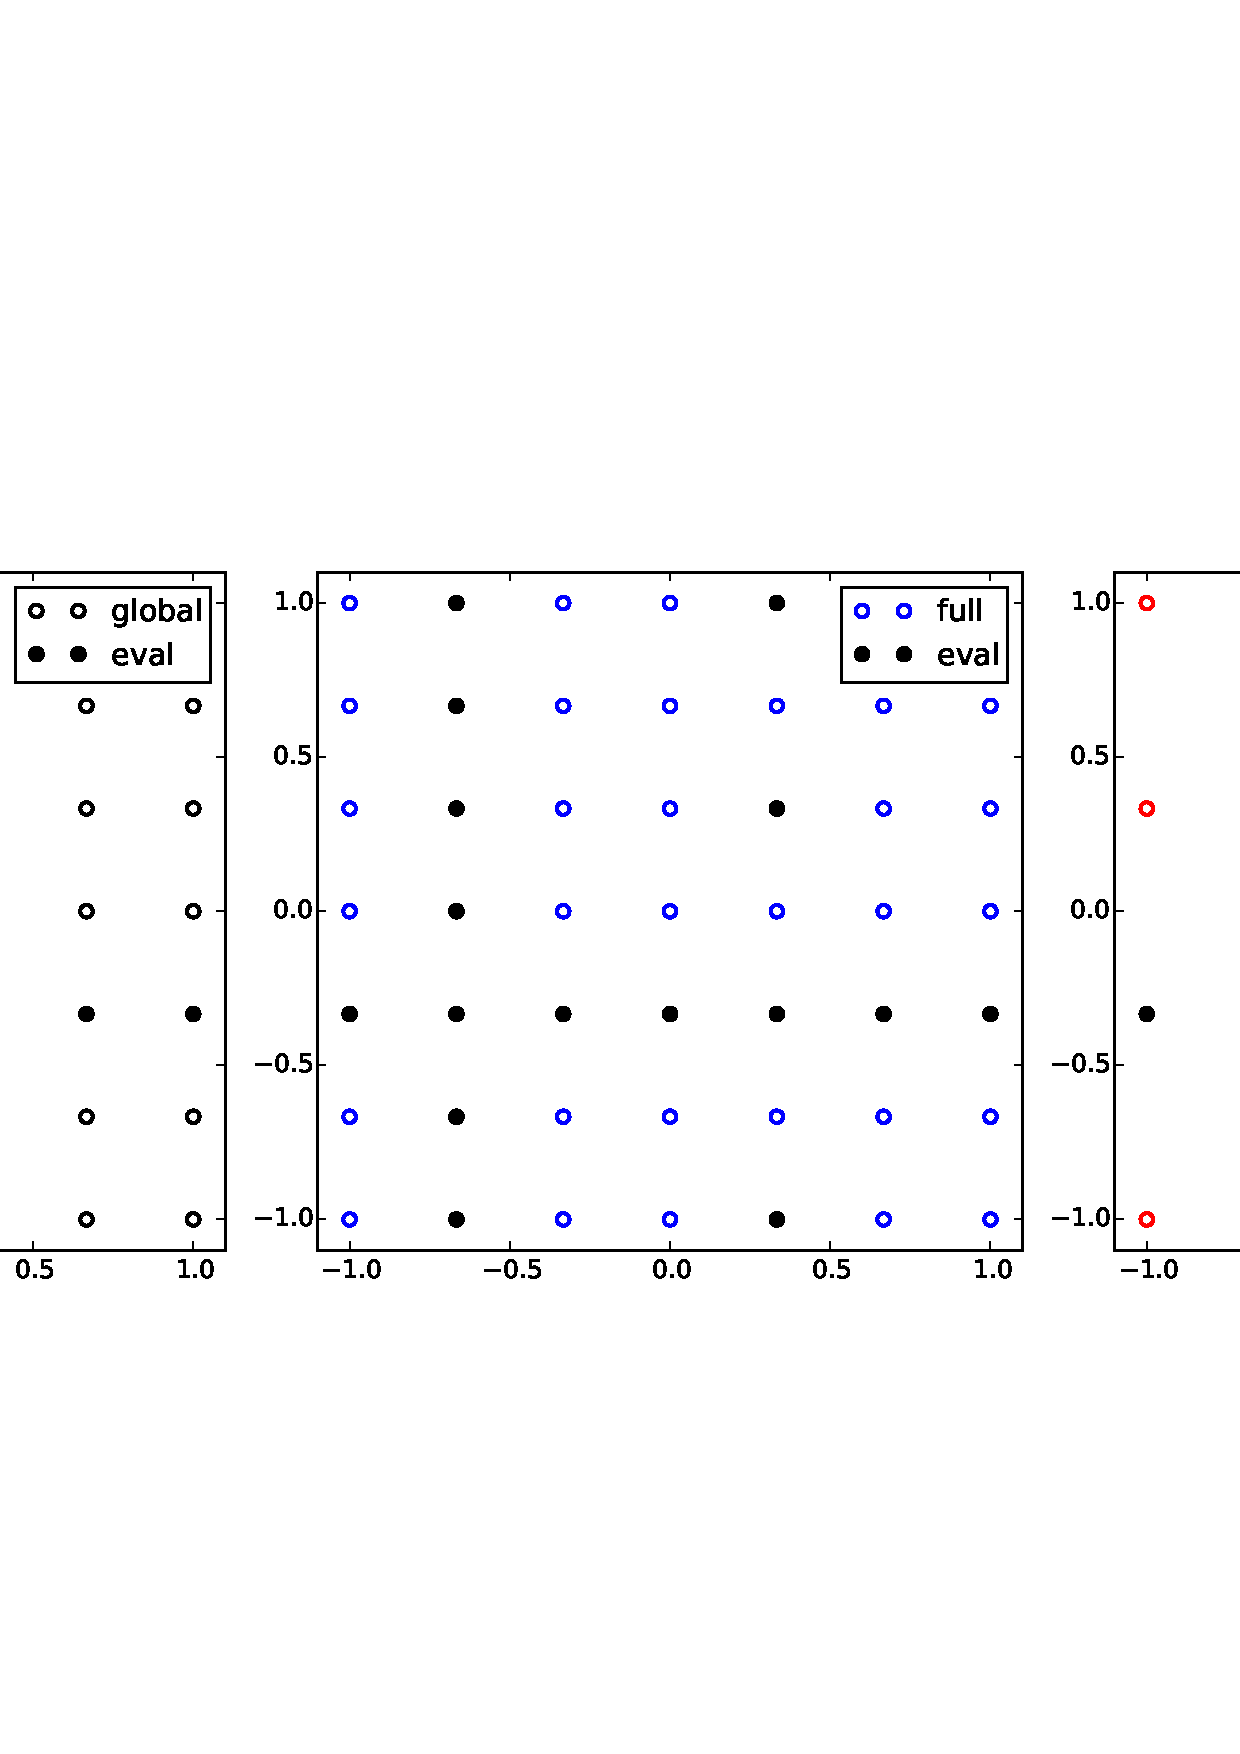
\includegraphics{TensorWrapperViews.pdf}
\caption{The global tensor and two of its views. The \code{full} view corresponds by default to the global tensor. The \code{coarse} is contained in the \code{full} view. The uniquely allocated values of the tensor are shown in the different views.}\end{figure}

The shape characteristics of the active view can be accessed through \code{TensorWrapper.get\_view\_shape()} and the corresponding commands for \code{ndim} and \code{size}. For example:

\begin{Verbatim}[commandchars=\\\{\}]
\PYG{g+gp}{\PYGZgt{}\PYGZgt{}\PYGZgt{} }\PYG{n}{TW}\PYG{o}{.}\PYG{n}{set\PYGZus{}active\PYGZus{}view}\PYG{p}{(}\PYG{l+s}{\PYGZsq{}}\PYG{l+s}{full}\PYG{l+s}{\PYGZsq{}}\PYG{p}{)}
\PYG{g+gp}{\PYGZgt{}\PYGZgt{}\PYGZgt{} }\PYG{n}{TW}\PYG{o}{.}\PYG{n}{get\PYGZus{}view\PYGZus{}shape}\PYG{p}{(}\PYG{p}{)}
\PYG{g+go}{(7, 7)}
\PYG{g+gp}{\PYGZgt{}\PYGZgt{}\PYGZgt{} }\PYG{n}{TW}\PYG{o}{.}\PYG{n}{get\PYGZus{}shape}\PYG{p}{(}\PYG{p}{)}
\PYG{g+go}{(7, 7)}
\PYG{g+gp}{\PYGZgt{}\PYGZgt{}\PYGZgt{} }\PYG{n}{TW}\PYG{o}{.}\PYG{n}{set\PYGZus{}active\PYGZus{}view}\PYG{p}{(}\PYG{l+s}{\PYGZsq{}}\PYG{l+s}{coarse}\PYG{l+s}{\PYGZsq{}}\PYG{p}{)}
\PYG{g+gp}{\PYGZgt{}\PYGZgt{}\PYGZgt{} }\PYG{n}{TW}\PYG{o}{.}\PYG{n}{get\PYGZus{}global\PYGZus{}shape}\PYG{p}{(}\PYG{p}{)}
\PYG{g+go}{(7, 7)}
\PYG{g+gp}{\PYGZgt{}\PYGZgt{}\PYGZgt{} }\PYG{n}{TW}\PYG{o}{.}\PYG{n}{get\PYGZus{}view\PYGZus{}shape}\PYG{p}{(}\PYG{p}{)}
\PYG{g+go}{(4, 4)}
\PYG{g+gp}{\PYGZgt{}\PYGZgt{}\PYGZgt{} }\PYG{n}{TW}\PYG{o}{.}\PYG{n}{get\PYGZus{}shape}\PYG{p}{(}\PYG{p}{)}
\PYG{g+go}{(4, 4)}
\PYG{g+gp}{\PYGZgt{}\PYGZgt{}\PYGZgt{} }\PYG{n}{TW}\PYG{o}{.}\PYG{n}{shape}
\PYG{g+go}{(4, 4)}
\end{Verbatim}


\subsection{Grid refinement}
\label{tw:grid-refinement}
The \emph{global} grid can be refined using the function \code{TensorWrapper.refine()}, provinding a grid which contains the previous one. This refinement does not alter the allocated data which is instead preserved and mapped to the new mesh.

\begin{Verbatim}[commandchars=\\\{\}]
\PYG{g+gp}{\PYGZgt{}\PYGZgt{}\PYGZgt{} }\PYG{n}{x\PYGZus{}ffine} \PYG{o}{=} \PYG{n}{np}\PYG{o}{.}\PYG{n}{linspace}\PYG{p}{(}\PYG{o}{\PYGZhy{}}\PYG{l+m+mi}{1}\PYG{p}{,}\PYG{l+m+mi}{1}\PYG{p}{,}\PYG{l+m+mi}{13}\PYG{p}{)}
\PYG{g+gp}{\PYGZgt{}\PYGZgt{}\PYGZgt{} }\PYG{n}{TW}\PYG{o}{.}\PYG{n}{refine}\PYG{p}{(}\PYG{p}{[}\PYG{n}{x\PYGZus{}ffine}\PYG{p}{]}\PYG{o}{*}\PYG{n}{d}\PYG{p}{)}
\end{Verbatim}
\begin{figure}[htbp]
\centering
\capstart

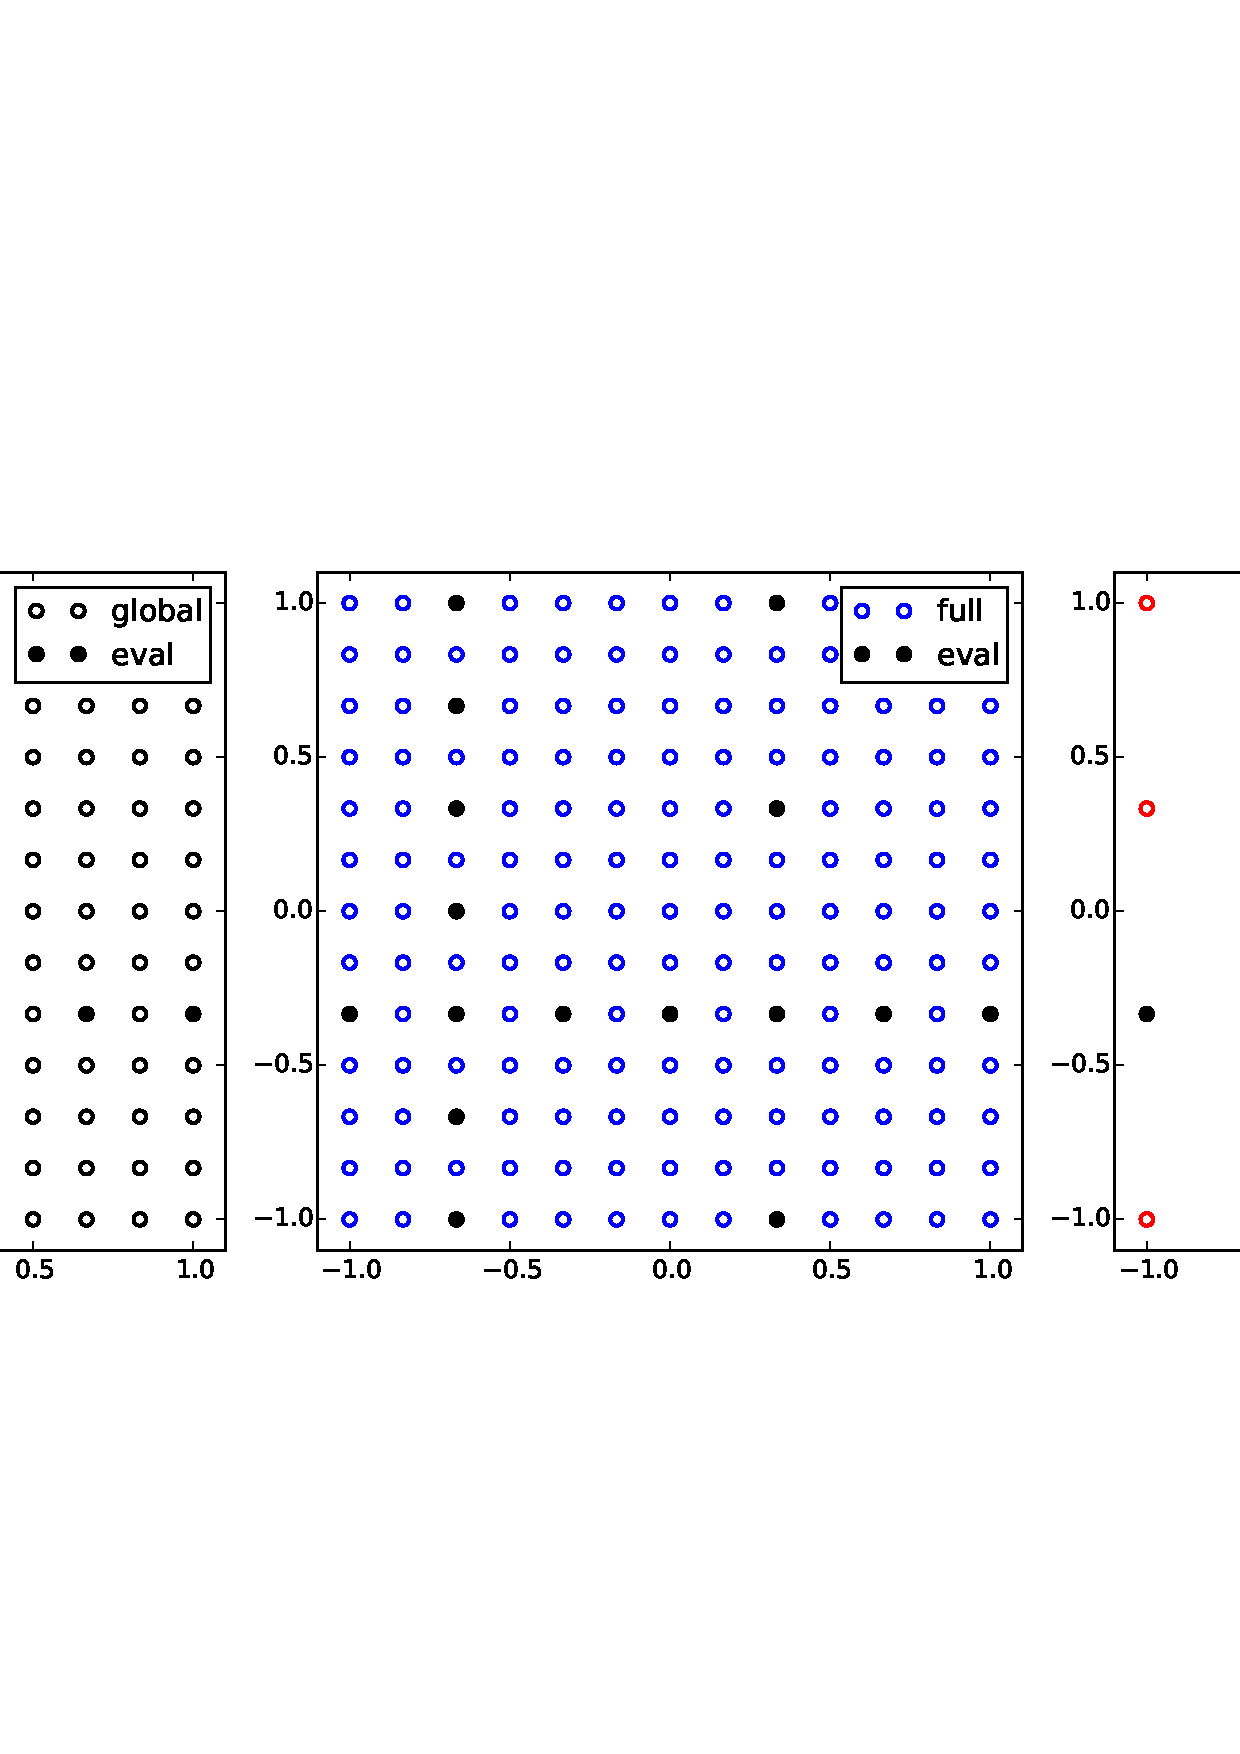
\includegraphics{TensorWrapperRefine.pdf}
\caption{The global tensor and the two views defined, after the grid refinement.}\end{figure}


\subsection{Quantics extension}
\label{tw:quantics-extension}
The quantics extension is used for extending the indices of the tesnor to the next power of \code{Q}. The extension is performed so that the last coordinate point is appended to the coordinate points the necessary number of times. In order to apply the extension on a particular view, one needs to activate the view and then use the method \code{TensorWrapper.set\_Q()}.

\begin{Verbatim}[commandchars=\\\{\}]
\PYG{g+gp}{\PYGZgt{}\PYGZgt{}\PYGZgt{} }\PYG{n}{TW}\PYG{o}{.}\PYG{n}{set\PYGZus{}active\PYGZus{}view}\PYG{p}{(}\PYG{l+s}{\PYGZsq{}}\PYG{l+s}{full}\PYG{l+s}{\PYGZsq{}}\PYG{p}{)}
\PYG{g+gp}{\PYGZgt{}\PYGZgt{}\PYGZgt{} }\PYG{n}{TW}\PYG{o}{.}\PYG{n}{get\PYGZus{}view\PYGZus{}shape}\PYG{p}{(}\PYG{p}{)}
\PYG{g+go}{(13, 13)}
\PYG{g+gp}{\PYGZgt{}\PYGZgt{}\PYGZgt{} }\PYG{n}{TW}\PYG{o}{.}\PYG{n}{get\PYGZus{}extended\PYGZus{}shape}\PYG{p}{(}\PYG{p}{)}
\PYG{g+go}{(13, 13)}
\PYG{g+gp}{\PYGZgt{}\PYGZgt{}\PYGZgt{} }\PYG{n}{TW}\PYG{o}{.}\PYG{n}{set\PYGZus{}Q}\PYG{p}{(}\PYG{l+m+mi}{2}\PYG{p}{)}
\PYG{g+gp}{\PYGZgt{}\PYGZgt{}\PYGZgt{} }\PYG{n}{TW}\PYG{o}{.}\PYG{n}{get\PYGZus{}extended\PYGZus{}shape}\PYG{p}{(}\PYG{p}{)}
\PYG{g+go}{(16, 16)}
\PYG{g+gp}{\PYGZgt{}\PYGZgt{}\PYGZgt{} }\PYG{n}{TW}\PYG{o}{.}\PYG{n}{get\PYGZus{}shape}\PYG{p}{(}\PYG{p}{)}
\PYG{g+go}{(16, 16)}
\PYG{g+gp}{\PYGZgt{}\PYGZgt{}\PYGZgt{} }\PYG{n}{TW}\PYG{o}{.}\PYG{n}{shape}
\PYG{g+go}{(16, 16)}
\end{Verbatim}

We can see that \code{TensorWrapper.get\_extended\_shape()} returns the same output of \code{TensorWrapper.get\_viw\_shape()} if no quantics extension has been applied.

Using the following code we can investigate the content of the extended tensor wrapper and plot it as shown in the following figure.

\begin{Verbatim}[commandchars=\\\{\}]
\PYG{g+gp}{\PYGZgt{}\PYGZgt{}\PYGZgt{} }\PYG{n}{A} \PYG{o}{=} \PYG{n}{TW}\PYG{p}{[}\PYG{p}{:}\PYG{p}{,}\PYG{p}{:}\PYG{p}{]}
\PYG{g+gp}{\PYGZgt{}\PYGZgt{}\PYGZgt{} }\PYG{k+kn}{import} \PYG{n+nn}{matplotlib.pyplot} \PYG{k+kn}{as} \PYG{n+nn}{plt}
\PYG{g+gp}{\PYGZgt{}\PYGZgt{}\PYGZgt{} }\PYG{n}{plt}\PYG{o}{.}\PYG{n}{figure}\PYG{p}{(}\PYG{n}{figsize}\PYG{o}{=}\PYG{p}{(}\PYG{l+m+mi}{6}\PYG{p}{,}\PYG{l+m+mi}{5}\PYG{p}{)}\PYG{p}{)}
\PYG{g+gp}{\PYGZgt{}\PYGZgt{}\PYGZgt{} }\PYG{n}{plt}\PYG{o}{.}\PYG{n}{imshow}\PYG{p}{(}\PYG{n}{A}\PYG{p}{,}\PYG{n}{interpolation}\PYG{o}{=}\PYG{l+s}{\PYGZsq{}}\PYG{l+s}{none}\PYG{l+s}{\PYGZsq{}}\PYG{p}{)}
\PYG{g+gp}{\PYGZgt{}\PYGZgt{}\PYGZgt{} }\PYG{n}{plt}\PYG{o}{.}\PYG{n}{tight\PYGZus{}layout}\PYG{p}{(}\PYG{p}{)}
\PYG{g+gp}{\PYGZgt{}\PYGZgt{}\PYGZgt{} }\PYG{n}{plt}\PYG{o}{.}\PYG{n}{show}\PYG{p}{(}\PYG{n+nb+bp}{False}\PYG{p}{)}
\end{Verbatim}
\begin{figure}[htbp]
\centering
\capstart

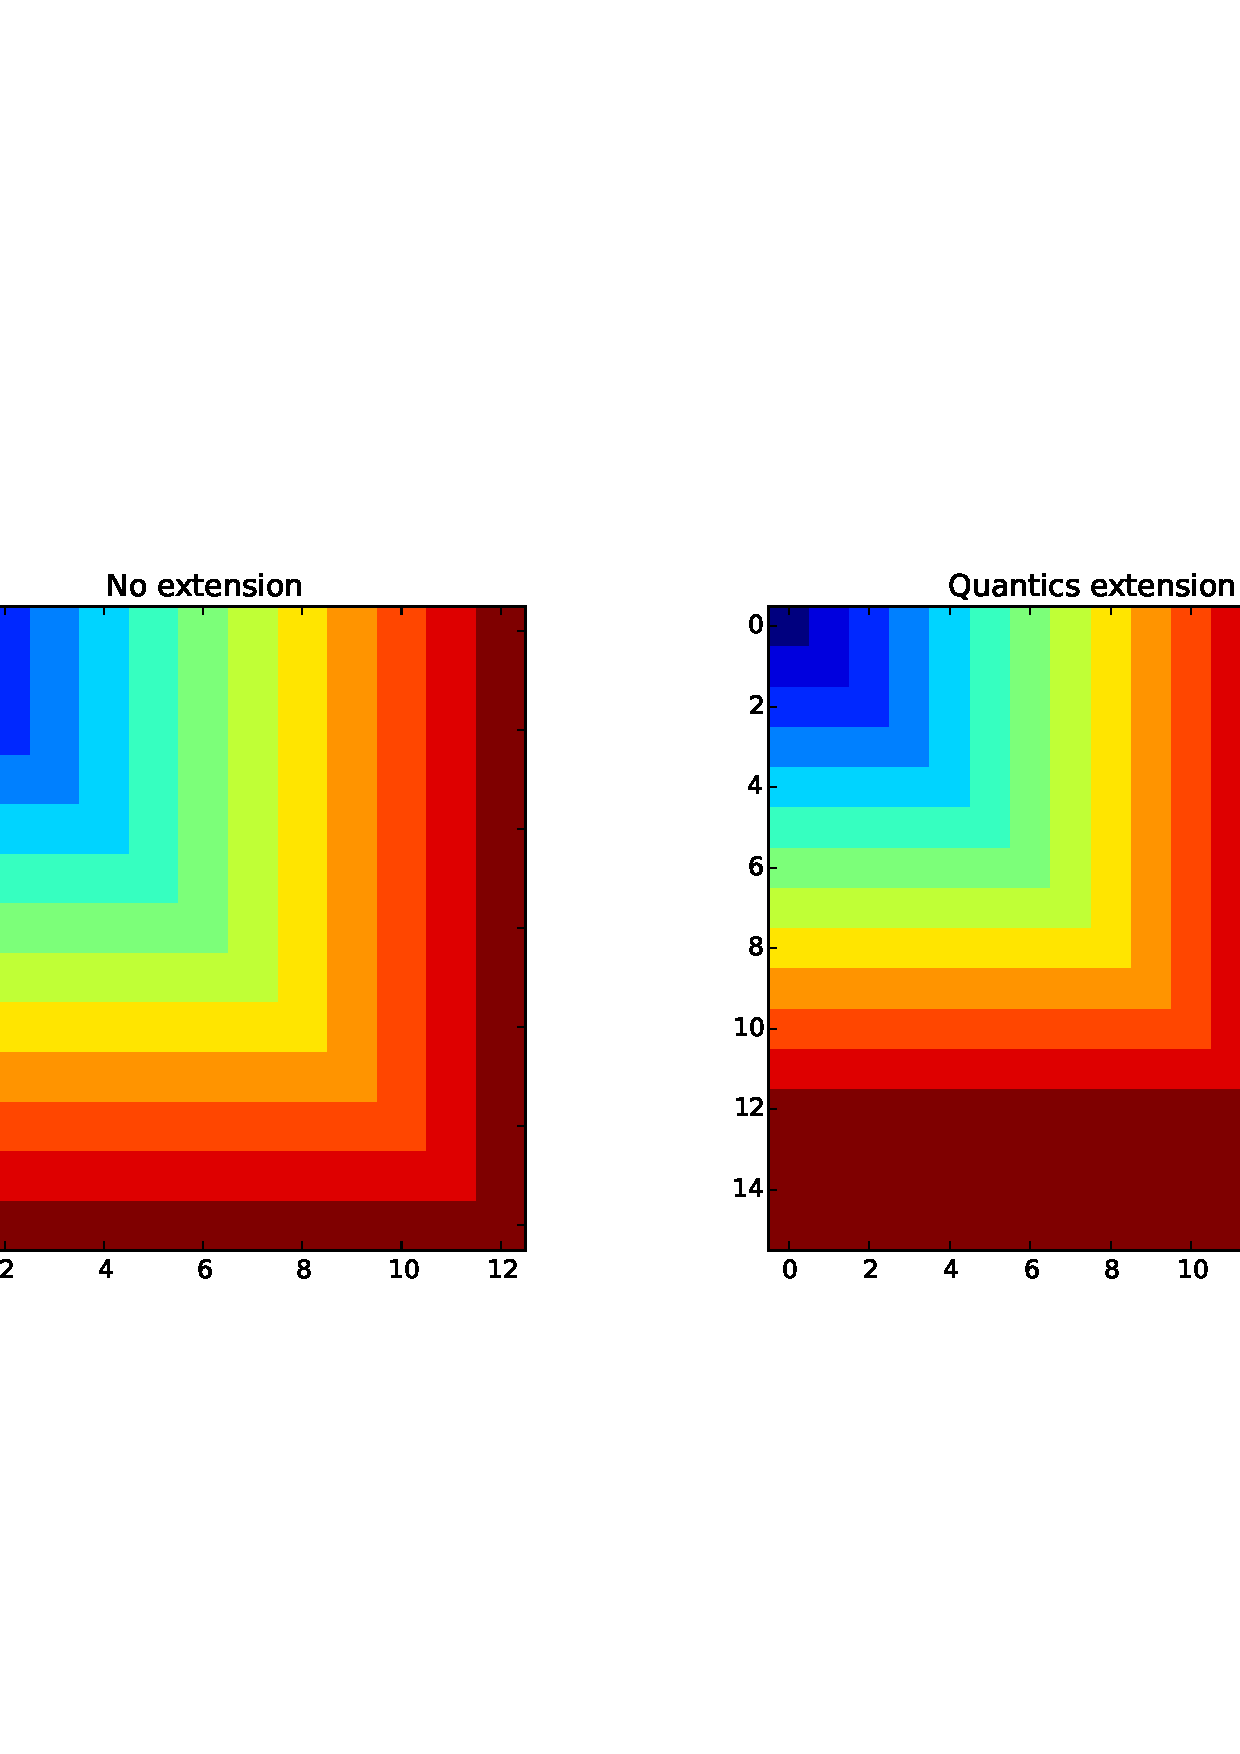
\includegraphics{TensorWrapperQExtension.pdf}
\caption{The \emph{Quantics} extension applied to the \code{full} view results in the repetition of its limit values in the tensor grid.}\end{figure}


\subsection{Reshape}
\label{tw:reshape}
The shape of each view can be changed as long as the size returned by \code{TensorWrapper.get\_extended\_size()} is unchanged. This means that if \emph{no quantics} extension has been applied, the size must correspond to \code{TensorWrapper.get\_view\_size()}. If a \emph{quantics} extension has been applied, the size must correspond to \code{TensorWrapper.get\_extended\_size()}.

For example let us reshape the \emph{quantics} extended \code{full} view of the tensor to the shape (4,16).

\begin{Verbatim}[commandchars=\\\{\}]
\PYG{g+gp}{\PYGZgt{}\PYGZgt{}\PYGZgt{} }\PYG{n}{TW}\PYG{o}{.}\PYG{n}{set\PYGZus{}active\PYGZus{}view}\PYG{p}{(}\PYG{l+s}{\PYGZsq{}}\PYG{l+s}{full}\PYG{l+s}{\PYGZsq{}}\PYG{p}{)}
\PYG{g+gp}{\PYGZgt{}\PYGZgt{}\PYGZgt{} }\PYG{n}{TW}\PYG{o}{.}\PYG{n}{reshape}\PYG{p}{(}\PYG{p}{(}\PYG{l+m+mi}{8}\PYG{p}{,}\PYG{l+m+mi}{32}\PYG{p}{)}\PYG{p}{)}
\PYG{g+gp}{\PYGZgt{}\PYGZgt{}\PYGZgt{} }\PYG{n}{TW}\PYG{o}{.}\PYG{n}{get\PYGZus{}extended\PYGZus{}shape}\PYG{p}{(}\PYG{p}{)}
\PYG{g+go}{(16, 16)}
\PYG{g+gp}{\PYGZgt{}\PYGZgt{}\PYGZgt{} }\PYG{n}{TW}\PYG{o}{.}\PYG{n}{get\PYGZus{}shape}\PYG{p}{(}\PYG{p}{)}
\PYG{g+go}{(8, 32)}
\PYG{g+gp}{\PYGZgt{}\PYGZgt{}\PYGZgt{} }\PYG{n}{TW}\PYG{o}{.}\PYG{n}{shape}
\PYG{g+go}{(8, 32)}
\end{Verbatim}

This results in the following reshaping of the tensor view:

\begin{Verbatim}[commandchars=\\\{\}]
\PYG{g+gp}{\PYGZgt{}\PYGZgt{}\PYGZgt{} }\PYG{n}{A} \PYG{o}{=} \PYG{n}{TW}\PYG{p}{[}\PYG{p}{:}\PYG{p}{,}\PYG{p}{:}\PYG{p}{]}
\PYG{g+gp}{\PYGZgt{}\PYGZgt{}\PYGZgt{} }\PYG{k+kn}{import} \PYG{n+nn}{matplotlib.pyplot} \PYG{k+kn}{as} \PYG{n+nn}{plt}
\PYG{g+gp}{\PYGZgt{}\PYGZgt{}\PYGZgt{} }\PYG{n}{plt}\PYG{o}{.}\PYG{n}{figure}\PYG{p}{(}\PYG{n}{figsize}\PYG{o}{=}\PYG{p}{(}\PYG{l+m+mi}{12}\PYG{p}{,}\PYG{l+m+mi}{5}\PYG{p}{)}\PYG{p}{)}
\PYG{g+gp}{\PYGZgt{}\PYGZgt{}\PYGZgt{} }\PYG{n}{plt}\PYG{o}{.}\PYG{n}{imshow}\PYG{p}{(}\PYG{n}{A}\PYG{p}{,}\PYG{n}{interpolation}\PYG{o}{=}\PYG{l+s}{\PYGZsq{}}\PYG{l+s}{none}\PYG{l+s}{\PYGZsq{}}\PYG{p}{)}
\PYG{g+gp}{\PYGZgt{}\PYGZgt{}\PYGZgt{} }\PYG{n}{plt}\PYG{o}{.}\PYG{n}{tight\PYGZus{}layout}\PYG{p}{(}\PYG{p}{)}
\PYG{g+gp}{\PYGZgt{}\PYGZgt{}\PYGZgt{} }\PYG{n}{plt}\PYG{o}{.}\PYG{n}{show}\PYG{p}{(}\PYG{n+nb+bp}{False}\PYG{p}{)}
\end{Verbatim}
\begin{figure}[htbp]
\centering
\capstart

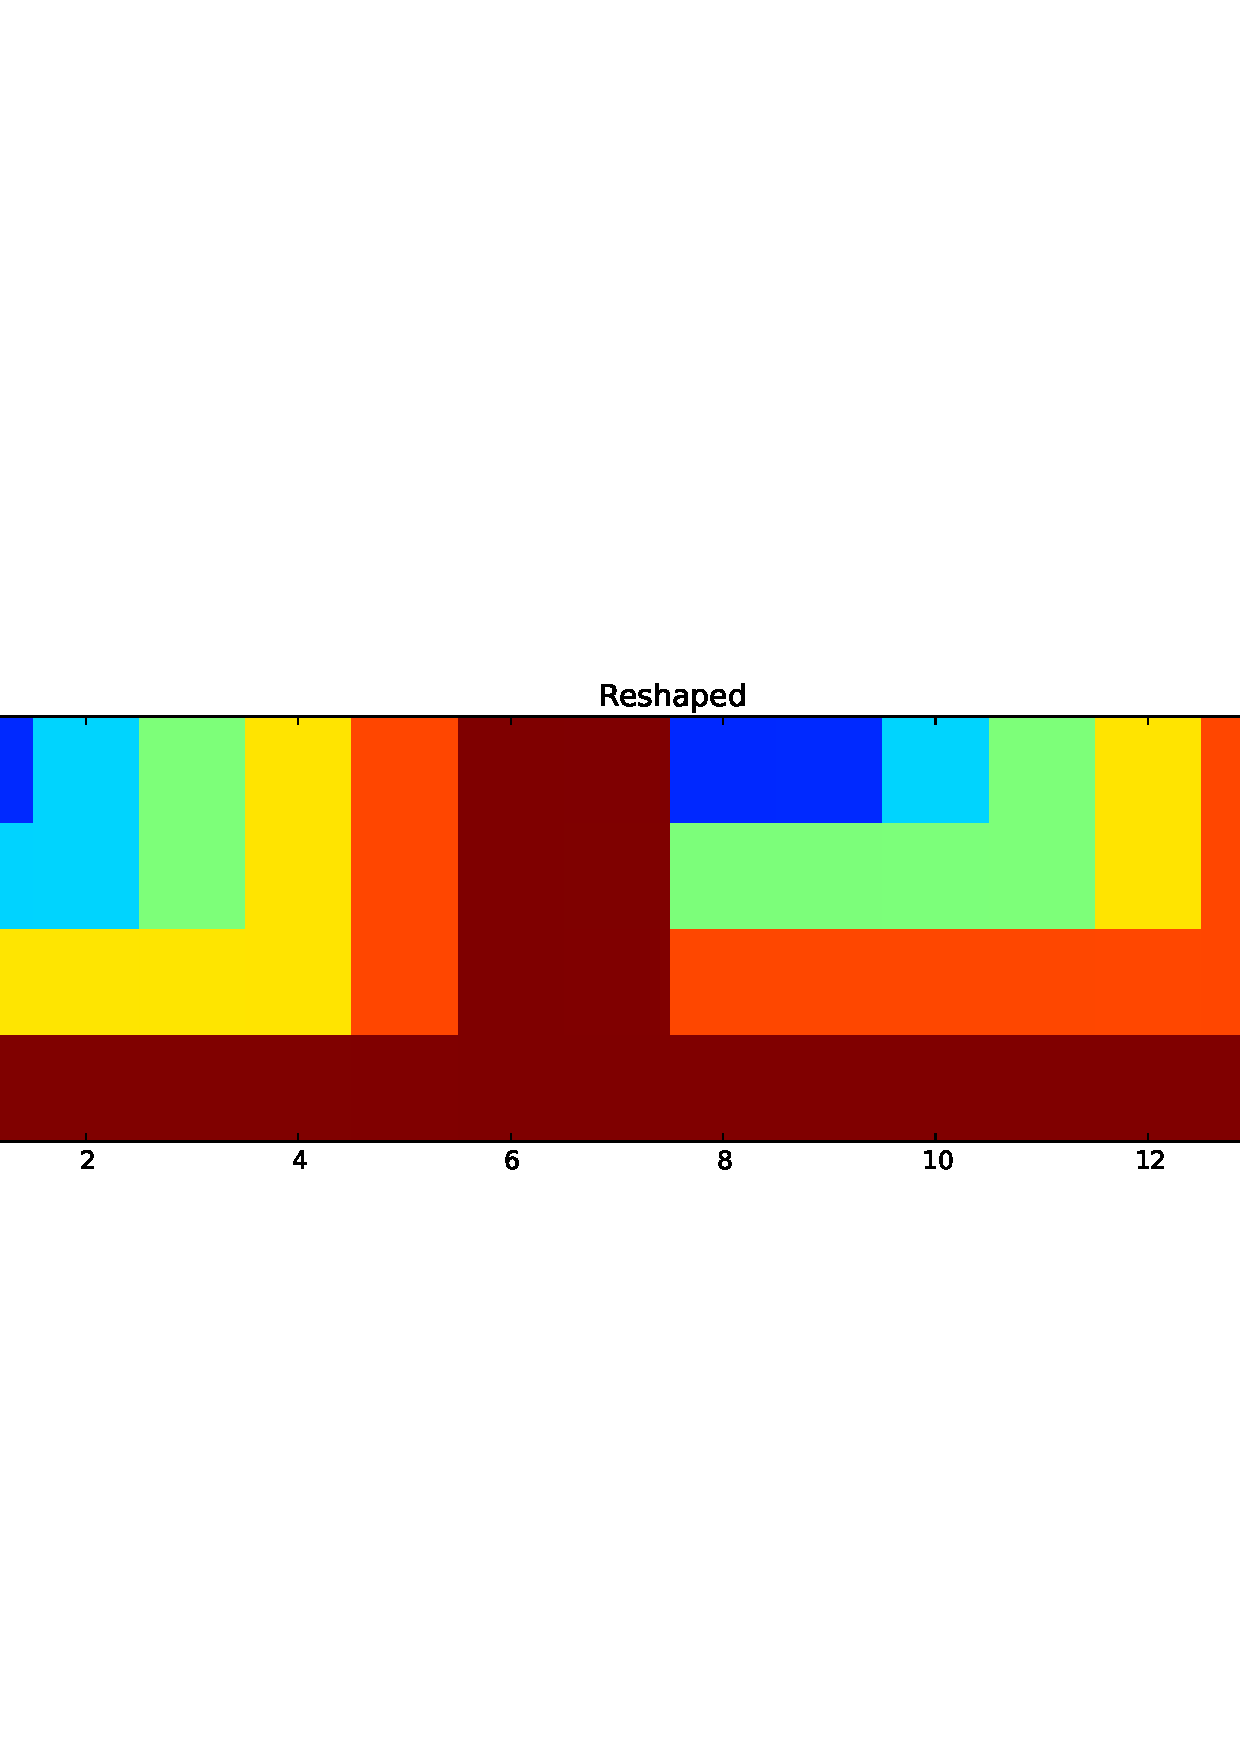
\includegraphics{TensorWrapperReshape.pdf}
\caption{Reshaping of the \emph{quantics} extended \code{full} view.}\end{figure}

The \emph{quantics} extension is used mainly to obtain a complete folding of base \code{Q}. In this case this is obtained by:

\begin{Verbatim}[commandchars=\\\{\}]
\PYG{g+gp}{\PYGZgt{}\PYGZgt{}\PYGZgt{} }\PYG{k+kn}{import} \PYG{n+nn}{math}
\PYG{g+gp}{\PYGZgt{}\PYGZgt{}\PYGZgt{} }\PYG{n}{TW}\PYG{o}{.}\PYG{n}{reshape}\PYG{p}{(} \PYG{p}{[}\PYG{l+m+mi}{2}\PYG{p}{]} \PYG{o}{*} \PYG{n+nb}{int}\PYG{p}{(}\PYG{n+nb}{round}\PYG{p}{(}\PYG{n}{math}\PYG{o}{.}\PYG{n}{log}\PYG{p}{(}\PYG{n}{TW}\PYG{o}{.}\PYG{n}{size}\PYG{p}{,}\PYG{l+m+mi}{2}\PYG{p}{)}\PYG{p}{)}\PYG{p}{)} \PYG{p}{)}
\PYG{g+gp}{\PYGZgt{}\PYGZgt{}\PYGZgt{} }\PYG{n}{TW}\PYG{o}{.}\PYG{n}{get\PYGZus{}extended\PYGZus{}shape}\PYG{p}{(}\PYG{p}{)}
\PYG{g+go}{(16, 16)}
\PYG{g+gp}{\PYGZgt{}\PYGZgt{}\PYGZgt{} }\PYG{n}{TW}\PYG{o}{.}\PYG{n}{get\PYGZus{}shape}\PYG{p}{(}\PYG{p}{)}
\PYG{g+go}{(2, 2, 2, 2, 2, 2, 2, 2)}
\PYG{g+gp}{\PYGZgt{}\PYGZgt{}\PYGZgt{} }\PYG{n}{TW}\PYG{o}{.}\PYG{n}{shape}
\PYG{g+go}{(2, 2, 2, 2, 2, 2, 2, 2)}
\end{Verbatim}

We finally can reset the shape to the \emph{view} shape using:

\begin{Verbatim}[commandchars=\\\{\}]
\PYG{g+gp}{\PYGZgt{}\PYGZgt{}\PYGZgt{} }\PYG{n}{TW}\PYG{o}{.}\PYG{n}{reset\PYGZus{}shape}\PYG{p}{(}\PYG{p}{)}
\end{Verbatim}


\subsection{Summary of shapes}
\label{tw:summary-of-shapes}
Information regarding several shape transformations are always hold in the data structure. A hierarchy of shapes is used. The top shape is the \textbf{global} shape. In the following table we list the different shapes, their description and the main functions related and affecting them.

\begin{tabulary}{\linewidth}{|L|L|L|}
\hline

\textbf{Shape}
 & 
\textbf{Description}
 & 
\textbf{Functions}
\\

Global
 & 
This is the underlying shape of the \code{TensorWrapper}.
 & 
\code{get\_global\_shape()}, \code{get\_global\_ndim()}, \code{get\_global\_size()}, \code{refine()}
\\

View
 & 
Multiple views can be defined for a \code{TensorWrapper}. The views are defined as nested grids into the global grid. The default view is called \code{full} and is defined automatically at construction time
 & 
\code{set\_view()}, \code{set\_active\_view()}, \code{get\_view\_shape()}, \code{get\_view\_ndim()}, \code{get\_view\_size()}, \code{refine()}
\\

Quantics Extended
 & 
Each view can be extended to the next power of \code{Q} in order to allow the \emph{quantics} folding {\hyperref[zrefs:khoromskij2011]{{[}2{]}}}{\hyperref[zrefs:khoromskij2010]{{[}1{]}}} of the tensor.
 & 
\code{set\_Q()}, \code{get\_extended\_shape()}, \code{get\_extended\_ndim()}, \code{get\_extended\_size()}
\\

Reshape
 & 
This is the result of the reshape of the tensor. If any of the preceding shape transformations have been applied, then the reshape is applied to the lowest transformation.
 & 
\code{reshape()}, \code{get\_shape()}, \code{get\_ndim()}, \code{get\_size()}, \code{shape}, \code{ndim}, \code{size}
\\
\hline\end{tabulary}


\begin{notice}{warning}{Warning:}
If a shape at any level is modified, every lower reshaping is automatically erased, due to possible inconsistency. For example, if a view is modified, any quantics extension and/or reshape of the view are reset.
\end{notice}

\begin{notice}{note}{Note:}
The \code{refine()} function erases all the quantics extensions and the reshapes of each view, but not the views themselves. Instead for each view, the \code{refine()} function updates the corresponding indices, fitting the old views to the new refinement.
\end{notice}


\subsection{Storage}
\label{tw:storage}
Instances of the class \code{TensorWrapper} can be stored in files and reloaded as needed. The class \code{TensorWrapper} extends the class \code{storable\_object}, which is responsible for storing objects in the {\hyperref[api-wttvec:module-TensorToolbox]{\code{TensorToolbox}}}.

For the sake of efficiency and readability of the code, the \code{TensorWrapper} is stored in two different files with a common file name \code{filename}:
\begin{itemize}
\item {} 
\code{filename.pkl} is a serialized version of the object thorugh the \href{https://docs.python.org/2/library/pickle.html}{pickle} library. The \code{TensorWrapper} serializes a minimal amount of auxiliary information needed for the definition of shapes, meshes, etc. The allocated data are not serialized using pickle, because when the amount of data is big, this would result in a very slow storage.

\item {} 
\code{filename.h5} is a binary file containing the allocated data of the \code{TensorWrapper}. This file is generated using \href{http://www.h5py.org/}{h5py} and results in fast loading, writing and appending of data.

\end{itemize}

Let us store the \code{TensorWrapper}, we have been using up to now.

\begin{Verbatim}[commandchars=\\\{\}]
\PYG{g+gp}{\PYGZgt{}\PYGZgt{}\PYGZgt{} }\PYG{n}{TW}\PYG{o}{.}\PYG{n}{set\PYGZus{}store\PYGZus{}location}\PYG{p}{(}\PYG{l+s}{\PYGZsq{}}\PYG{l+s}{tensorwrapper}\PYG{l+s}{\PYGZsq{}}\PYG{p}{)}
\PYG{g+gp}{\PYGZgt{}\PYGZgt{}\PYGZgt{} }\PYG{n}{TW}\PYG{o}{.}\PYG{n}{store}\PYG{p}{(}\PYG{n}{force}\PYG{o}{=}\PYG{n+nb+bp}{True}\PYG{p}{)}
\end{Verbatim}

Check that the files have been stored:

\begin{Verbatim}[commandchars=\\\{\}]
\PYG{n+nv}{\PYGZdl{} }ls
tensorwrapper.h5  tensorwrapper.pkl  WrapperExample.py
\end{Verbatim}

Let's now reload the \code{TensorWrapper}:

\begin{Verbatim}[commandchars=\\\{\}]
\PYG{g+gp}{\PYGZgt{}\PYGZgt{}\PYGZgt{} }\PYG{n}{TW} \PYG{o}{=} \PYG{n}{TT}\PYG{o}{.}\PYG{n}{load}\PYG{p}{(}\PYG{l+s}{\PYGZsq{}}\PYG{l+s}{tensorwrapper}\PYG{l+s}{\PYGZsq{}}\PYG{p}{)}
\end{Verbatim}

The storage of the tensor wrapper can also be triggered using a timer. This is mostly useful when many time consuming computations need to be performed in order to allocate the desired entries of the tensor, and one wants to have always a backup copy of the data. The trigger for the storage is checked any time a new entry needs to be allocated fo storage.

For example, we can set the storage frequency to 5s:

\begin{Verbatim}[commandchars=\\\{\}]
\PYG{g+gp}{\PYGZgt{}\PYGZgt{}\PYGZgt{} }\PYG{k+kn}{import} \PYG{n+nn}{time}
\PYG{g+gp}{\PYGZgt{}\PYGZgt{}\PYGZgt{} }\PYG{n}{TW}\PYG{o}{.}\PYG{n}{data} \PYG{o}{=} \PYG{p}{\PYGZob{}}\PYG{p}{\PYGZcb{}}
\PYG{g+gp}{\PYGZgt{}\PYGZgt{}\PYGZgt{} }\PYG{n}{TW}\PYG{p}{[}\PYG{l+m+mi}{1}\PYG{p}{,}\PYG{l+m+mi}{2}\PYG{p}{]}
\PYG{g+gp}{\PYGZgt{}\PYGZgt{}\PYGZgt{} }\PYG{n}{TW}\PYG{o}{.}\PYG{n}{set\PYGZus{}store\PYGZus{}freq}\PYG{p}{(} \PYG{l+m+mi}{5} \PYG{p}{)}
\PYG{g+gp}{\PYGZgt{}\PYGZgt{}\PYGZgt{} }\PYG{n}{time}\PYG{o}{.}\PYG{n}{sleep}\PYG{p}{(}\PYG{l+m+mf}{6.0}\PYG{p}{)}
\PYG{g+gp}{\PYGZgt{}\PYGZgt{}\PYGZgt{} }\PYG{n}{TW}\PYG{p}{[}\PYG{l+m+mi}{3}\PYG{p}{,}\PYG{l+m+mi}{5}\PYG{p}{]}
\end{Verbatim}

Checking the output we see:

\begin{Verbatim}[commandchars=\\\{\}]
\PYG{n+nv}{\PYGZdl{} }ls
tensorwrapper.h5      tensorwrapper.pkl     WrapperExample.py
tensorwrapper.h5.old  tensorwrapper.pkl.old
\end{Verbatim}

where the files \code{.pkl} and \code{.h5} are the files stored when the time-trigger is activated, while the files \code{.pkl.old} and \code{h5.old} are backup files containing the data stored in the previous example.


\section{Tensor Train Vectors}
\label{ttvec:tensor-train-vectors}\label{ttvec::doc}

\section{Tensor Train Matrices}
\label{ttmat:tensor-train-matrices}\label{ttmat::doc}

\section{Quantics Tensor Train Vectors}
\label{qttvec::doc}\label{qttvec:quantics-tensor-train-vectors}

\section{Quantics Tensor Train Matrices}
\label{qttmat::doc}\label{qttmat:quantics-tensor-train-matrices}

\section{Spectral Tensor Train}
\label{stt:spectral-tensor-train}\label{stt::doc}

\section{Multi-linear algebra}
\label{multilinalg:multi-linear-algebra}\label{multilinalg::doc}

\chapter{API}
\label{api:api}\label{api::doc}

\section{Tensor Wrapper}
\label{api-tw:tensor-wrapper}\label{api-tw::doc}\label{api-tw:module-TensorToolbox}\index{TensorToolbox (module)}\index{TensorWrapper (class in TensorToolbox.core)}

\begin{fulllineitems}
\phantomsection\label{api-tw:TensorToolbox.core.TensorWrapper}\pysiglinewithargsret{\strong{class }\code{TensorToolbox.core.}\bfcode{TensorWrapper}}{\emph{f}, \emph{X}, \emph{params=None}, \emph{W=None}, \emph{twtype='array'}, \emph{data=None}, \emph{dtype=\textless{}type `object'\textgreater{}}, \emph{store\_file='`}, \emph{store\_object=None}, \emph{store\_freq=None}, \emph{store\_overwrite=False}, \emph{empty=False}, \emph{maxprocs=None}, \emph{marshal\_f=True}}{}
A tensor wrapper is a data structure W that given a multi-dimensional scalar function f(X,params), and a set of coordinates \{\{x1\}\_i1,\{x2\}\_i2,..,\{xd\}\_id\} indexed by the multi index \{i1,..,id\}, let you access f(x1\_i1,..,xd\_id) by W{[}i1,..,id{]}. The function evaluations are performed ``as needed'' and stored for future accesses.
\begin{quote}\begin{description}
\item[{Parameters}] \leavevmode\begin{itemize}
\item {} 
\textbf{f} -- multi-dimensional scalar function of type f(x,params), x being a list.

\item {} 
\textbf{X} (\href{http://docs.python.org/library/functions.html\#list}{\emph{list}}) -- list of arrays with coordinates for each dimension

\item {} 
\textbf{params} (\href{http://docs.python.org/library/functions.html\#tuple}{\emph{tuple}}) -- parameters to be passed to function f

\item {} 
\textbf{W} (\href{http://docs.python.org/library/functions.html\#list}{\emph{list}}) -- list of arrays with weights for each dimension

\item {} 
\textbf{twtype} (\href{http://docs.python.org/library/string.html\#module-string}{\emph{string}}) -- `array' values are stored whenever computed, `view' values are never stored and function f is always called

\item {} 
\textbf{data} (\href{http://docs.python.org/library/stdtypes.html\#dict}{\emph{dict}}) -- initialization data of the Tensor Wrapper (already computed entries)

\item {} 
\textbf{dtype} (\href{http://docs.python.org/library/functions.html\#type}{\emph{type}}) -- type of output to be expected from f

\item {} 
\textbf{store\_file} (\href{http://docs.python.org/library/functions.html\#str}{\emph{str}}) -- file where to store the data

\item {} 
\textbf{store\_object} (\href{http://docs.python.org/library/functions.html\#object}{\emph{object}}) -- a storable object that must be stored in place of the TensorWrapper

\item {} 
\textbf{store\_freq} (\href{http://docs.python.org/library/functions.html\#bool}{\emph{bool}}) -- how frequently to store the TensorWrapper (seconds)

\item {} 
\textbf{store\_overwrite} (\href{http://docs.python.org/library/functions.html\#bool}{\emph{bool}}) -- whether to overwrite pre-existing files.

\item {} 
\textbf{empty} (\href{http://docs.python.org/library/functions.html\#bool}{\emph{bool}}) -- Creates an instance without initializing it. All the content can be initialized using the \code{setstate()} function.

\item {} 
\textbf{maxprocs} (\href{http://docs.python.org/library/functions.html\#int}{\emph{int}}) -- Number of processors to be used in the function evaluation (MPI)

\item {} 
\textbf{marshal\_f} (\href{http://docs.python.org/library/functions.html\#bool}{\emph{bool}}) -- whether to marshal the function or not

\end{itemize}

\end{description}\end{quote}

Several shape parameters are used by the TensorWrapper in order to keep track of reshaping and slicings, without affecting the underlying shape of the tensor which is always preserved. The following table lists the existing shapes and their meaning.

\begin{tabulary}{\linewidth}{|L|L|L|}
\hline
\textsf{\relax 
Shape attribute/function
} & \textsf{\relax 
Applied transformations (ordered)
} & \textsf{\relax 
Description
}\\
\hline
\code{get\_global\_shape()}
 & 
None
 & 
The original shape of the tensor. This shape can be modified only  through a refinement of the grid using the function \code{refine()}.
\\

\code{get\_view\_shape()}
 & 
VIEW
 & 
The particular view of the tensor, defined by the view in \code{TensorWrapper.maps} set active using \code{set\_active\_view()}.
\\

\code{get\_extended\_shape()}
 & 
VIEW, QUANTICS
 & 
The shape of the extended tensor in order to allow for the quantics folding with basis \code{TensorWrapper.Q}.
\\

\code{get\_ghost\_shape()}
 & 
VIEW, QUANTICS, RESHAPE
 & 
The shape of the tensor reshaped using \code{reshape()}. If a Quantics folding is pre-applied, then the reshape is on the extended shape.
\\

\code{get\_shape()}
 & 
VIEW, QUANTICS, RESHAPE, FIX\_IDXS
 & 
The shape of the tensor with \code{fix\_indices()} and \code{release\_indices()}. This is the view that is always used when the tensor is accessed through the function {\hyperref[api-tw:TensorToolbox.TensorWrapper.__getitem__]{\code{\_\_getitem\_\_()}}} (i.e. \code{TW{[}...{]}})
\\
\hline\end{tabulary}

\index{\_\_getitem\_\_() (TensorToolbox.TensorWrapper method)}

\begin{fulllineitems}
\phantomsection\label{api-tw:TensorToolbox.TensorWrapper.__getitem__}\pysiglinewithargsret{\bfcode{\_\_getitem\_\_}}{\emph{idxs\_in}}{}
\end{fulllineitems}

\index{extended\_is\_view() (TensorToolbox.core.TensorWrapper method)}

\begin{fulllineitems}
\phantomsection\label{api-tw:TensorToolbox.core.TensorWrapper.extended_is_view}\pysiglinewithargsret{\bfcode{extended\_is\_view}}{\emph{idxs}}{}~\begin{quote}\begin{description}
\item[{Returns}] \leavevmode
True if the idxs is in the view shape. False if it is outside

\end{description}\end{quote}

\end{fulllineitems}

\index{fix\_indices() (TensorToolbox.core.TensorWrapper method)}

\begin{fulllineitems}
\phantomsection\label{api-tw:TensorToolbox.core.TensorWrapper.fix_indices}\pysiglinewithargsret{\bfcode{fix\_indices}}{\emph{idxs}, \emph{dims}}{}
Fix some of the indices in the tensor wrapper and reshape/resize it accordingly. The internal storage of the data is still done with respect to the global indices, but once some indices are fixed, the TensorWrapper can be accessed using just the remaining free indices.
\begin{quote}\begin{description}
\item[{Parameters}] \leavevmode\begin{itemize}
\item {} 
\textbf{idxs} (\href{http://docs.python.org/library/functions.html\#list}{\emph{list}}) -- list of indices to be fixed

\item {} 
\textbf{dims} (\href{http://docs.python.org/library/functions.html\#list}{\emph{list}}) -- list of dimensions to which the indices refer to

\end{itemize}

\end{description}\end{quote}

\end{fulllineitems}

\index{get\_extended\_ndim() (TensorToolbox.core.TensorWrapper method)}

\begin{fulllineitems}
\phantomsection\label{api-tw:TensorToolbox.core.TensorWrapper.get_extended_ndim}\pysiglinewithargsret{\bfcode{get\_extended\_ndim}}{}{}
If the quantics folding has been performed on the current view, then this returns the number of dimensions of the extended tensor to the next power of Q. If the folding has not been performed, this returns an error.

\end{fulllineitems}

\index{get\_extended\_shape() (TensorToolbox.core.TensorWrapper method)}

\begin{fulllineitems}
\phantomsection\label{api-tw:TensorToolbox.core.TensorWrapper.get_extended_shape}\pysiglinewithargsret{\bfcode{get\_extended\_shape}}{}{}
If the quantics folding has been performed on the current view, then this returns the shape of the extended tensor to the next power of Q. If the folding has not been performed, this returns the view shape.

\end{fulllineitems}

\index{get\_extended\_size() (TensorToolbox.core.TensorWrapper method)}

\begin{fulllineitems}
\phantomsection\label{api-tw:TensorToolbox.core.TensorWrapper.get_extended_size}\pysiglinewithargsret{\bfcode{get\_extended\_size}}{}{}
If the quantics folding has been performed on the current view, then this returns the size of the extended tensor to the next power of Q. If the folding has not been performed, this returns an error.

\end{fulllineitems}

\index{get\_ghost\_ndim() (TensorToolbox.core.TensorWrapper method)}

\begin{fulllineitems}
\phantomsection\label{api-tw:TensorToolbox.core.TensorWrapper.get_ghost_ndim}\pysiglinewithargsret{\bfcode{get\_ghost\_ndim}}{}{}
If the \code{ghost\_shape} is set for this view, then it returns the number of dimensions obtained after quantics folding by the function \code{set\_Q()} or after reshaping by the function \code{reshape()}. Otherwise the number of dimensions of the view is returned.

\end{fulllineitems}

\index{get\_ghost\_shape() (TensorToolbox.core.TensorWrapper method)}

\begin{fulllineitems}
\phantomsection\label{api-tw:TensorToolbox.core.TensorWrapper.get_ghost_shape}\pysiglinewithargsret{\bfcode{get\_ghost\_shape}}{}{}
If the \code{ghost\_shape} is set for this view, then it returns the shape obtained after quantics folding by the function \code{set\_Q()} or after reshaping by the function \code{reshape()}. Otherwise the shape of the extended shape is returned.

\end{fulllineitems}

\index{get\_ghost\_size() (TensorToolbox.core.TensorWrapper method)}

\begin{fulllineitems}
\phantomsection\label{api-tw:TensorToolbox.core.TensorWrapper.get_ghost_size}\pysiglinewithargsret{\bfcode{get\_ghost\_size}}{}{}
If the \code{ghost\_shape} is set for this view, then it returns the size obtained after quantics folding by the function \code{set\_Q()} or after reshaping by the function \code{reshape()}. Otherwise the size of the view is returned.

\end{fulllineitems}

\index{get\_global\_ndim() (TensorToolbox.core.TensorWrapper method)}

\begin{fulllineitems}
\phantomsection\label{api-tw:TensorToolbox.core.TensorWrapper.get_global_ndim}\pysiglinewithargsret{\bfcode{get\_global\_ndim}}{}{}
Always returns the ndim of the underlying tensor

\end{fulllineitems}

\index{get\_global\_shape() (TensorToolbox.core.TensorWrapper method)}

\begin{fulllineitems}
\phantomsection\label{api-tw:TensorToolbox.core.TensorWrapper.get_global_shape}\pysiglinewithargsret{\bfcode{get\_global\_shape}}{}{}
Always returns the shape of the underlying tensor

\end{fulllineitems}

\index{get\_global\_size() (TensorToolbox.core.TensorWrapper method)}

\begin{fulllineitems}
\phantomsection\label{api-tw:TensorToolbox.core.TensorWrapper.get_global_size}\pysiglinewithargsret{\bfcode{get\_global\_size}}{}{}
Always returns the size of the underlying tensor

\end{fulllineitems}

\index{get\_ndim() (TensorToolbox.core.TensorWrapper method)}

\begin{fulllineitems}
\phantomsection\label{api-tw:TensorToolbox.core.TensorWrapper.get_ndim}\pysiglinewithargsret{\bfcode{get\_ndim}}{}{}
Always returns the number of dimensions of the tensor view

\end{fulllineitems}

\index{get\_shape() (TensorToolbox.core.TensorWrapper method)}

\begin{fulllineitems}
\phantomsection\label{api-tw:TensorToolbox.core.TensorWrapper.get_shape}\pysiglinewithargsret{\bfcode{get\_shape}}{}{}
Always returns the shape of the actual tensor view

\end{fulllineitems}

\index{get\_size() (TensorToolbox.core.TensorWrapper method)}

\begin{fulllineitems}
\phantomsection\label{api-tw:TensorToolbox.core.TensorWrapper.get_size}\pysiglinewithargsret{\bfcode{get\_size}}{}{}
Always returns the size of the tensor view

\end{fulllineitems}

\index{get\_view\_ndim() (TensorToolbox.core.TensorWrapper method)}

\begin{fulllineitems}
\phantomsection\label{api-tw:TensorToolbox.core.TensorWrapper.get_view_ndim}\pysiglinewithargsret{\bfcode{get\_view\_ndim}}{}{}
Always returns the ndim of the current view

\end{fulllineitems}

\index{get\_view\_shape() (TensorToolbox.core.TensorWrapper method)}

\begin{fulllineitems}
\phantomsection\label{api-tw:TensorToolbox.core.TensorWrapper.get_view_shape}\pysiglinewithargsret{\bfcode{get\_view\_shape}}{}{}
Always returns the shape of the current view

\end{fulllineitems}

\index{get\_view\_size() (TensorToolbox.core.TensorWrapper method)}

\begin{fulllineitems}
\phantomsection\label{api-tw:TensorToolbox.core.TensorWrapper.get_view_size}\pysiglinewithargsret{\bfcode{get\_view\_size}}{}{}
Always returns the size of the current view

\end{fulllineitems}

\index{ghost\_to\_global() (TensorToolbox.core.TensorWrapper method)}

\begin{fulllineitems}
\phantomsection\label{api-tw:TensorToolbox.core.TensorWrapper.ghost_to_global}\pysiglinewithargsret{\bfcode{ghost\_to\_global}}{\emph{idxs}}{}
This maps the index from the current ghost shape of the view to the global shape.
\begin{quote}\begin{description}
\item[{Parameters}] \leavevmode
\textbf{idxs\_in} (\href{http://docs.python.org/library/functions.html\#list}{\emph{list}}) -- list of indices to be transformed

\end{description}\end{quote}

\begin{notice}{note}{Note:}
no slicing is admitted here. Preprocess \code{idxs} with \code{expand\_idxs()} if slicing is required.
\end{notice}

\end{fulllineitems}

\index{ghost\_to\_view() (TensorToolbox.core.TensorWrapper method)}

\begin{fulllineitems}
\phantomsection\label{api-tw:TensorToolbox.core.TensorWrapper.ghost_to_view}\pysiglinewithargsret{\bfcode{ghost\_to\_view}}{\emph{idxs}}{}
This maps the index from the current ghost shape of the view to the view shape.
\begin{quote}\begin{description}
\item[{Parameters}] \leavevmode
\textbf{idxs\_in} (\href{http://docs.python.org/library/functions.html\#list}{\emph{list}}) -- list of indices to be transformed

\end{description}\end{quote}

\begin{notice}{note}{Note:}
no slicing is admitted here. Preprocess \code{idxs} with \code{expand\_idxs()} if slicing is required.
\end{notice}

\end{fulllineitems}

\index{global\_to\_ghost() (TensorToolbox.core.TensorWrapper method)}

\begin{fulllineitems}
\phantomsection\label{api-tw:TensorToolbox.core.TensorWrapper.global_to_ghost}\pysiglinewithargsret{\bfcode{global\_to\_ghost}}{\emph{idxs}}{}
This maps the index from the global shape to the ghost shape.
\begin{quote}\begin{description}
\item[{Parameters}] \leavevmode
\textbf{idxs} (\href{http://docs.python.org/library/functions.html\#list}{\emph{list}}) -- list of indices to be transformed

\end{description}\end{quote}

\begin{notice}{note}{Note:}
no slicing is admitted here. Preprocess \code{idxs} with \code{expand\_idxs()} if slicing is required.
\end{notice}

For \code{TensorWrapper()} \code{A}, this corresponds to:

\begin{Verbatim}[commandchars=\\\{\}]
\PYG{g+gp}{\PYGZgt{}\PYGZgt{}\PYGZgt{} }\PYG{n}{A}\PYG{o}{.}\PYG{n}{view\PYGZus{}to\PYGZus{}ghost}\PYG{p}{(} \PYG{n}{A}\PYG{o}{.}\PYG{n}{global\PYGZus{}to\PYGZus{}view}\PYG{p}{(} \PYG{n}{idxs} \PYG{p}{)} \PYG{p}{)}
\end{Verbatim}

\end{fulllineitems}

\index{global\_to\_view() (TensorToolbox.core.TensorWrapper method)}

\begin{fulllineitems}
\phantomsection\label{api-tw:TensorToolbox.core.TensorWrapper.global_to_view}\pysiglinewithargsret{\bfcode{global\_to\_view}}{\emph{idxs}}{}
This maps the index from the global shape to the view shape.
\begin{quote}\begin{description}
\item[{Parameters}] \leavevmode
\textbf{idxs} (\href{http://docs.python.org/library/functions.html\#tuple}{\emph{tuple}}) -- tuple representing an index to be transformed.

\end{description}\end{quote}

\begin{notice}{note}{Note:}
no slicing is admitted here. Preprocess \code{idxs} with \code{expand\_idxs()} if slicing is required.
\end{notice}

\begin{notice}{note}{Note:}
this returns an error if the \code{idxs} do not belong to the index mapping of the current view.
\end{notice}

\end{fulllineitems}

\index{refine() (TensorToolbox.core.TensorWrapper method)}

\begin{fulllineitems}
\phantomsection\label{api-tw:TensorToolbox.core.TensorWrapper.refine}\pysiglinewithargsret{\bfcode{refine}}{\emph{X\_new}, \emph{tol=None}}{}
Refine the global discretization. The new discretization must contain the old one.

This function takes care of updating all the indices in the global view as well in all the other views.
\begin{quote}\begin{description}
\item[{Parameters}] \leavevmode\begin{itemize}
\item {} 
\textbf{X\_new} (\href{http://docs.python.org/library/functions.html\#list}{\emph{list}}) -- list of coordinates of the new refinement

\item {} 
\textbf{tol} (\href{http://docs.python.org/library/functions.html\#float}{\emph{float}}) -- tolerance for the matching of coordinates

\end{itemize}

\end{description}\end{quote}

\begin{notice}{warning}{Warning:}
Any existing reshaping of the views is discarded.
\end{notice}

\end{fulllineitems}

\index{release\_indices() (TensorToolbox.core.TensorWrapper method)}

\begin{fulllineitems}
\phantomsection\label{api-tw:TensorToolbox.core.TensorWrapper.release_indices}\pysiglinewithargsret{\bfcode{release\_indices}}{}{}
Release all the indices in the tensor wrapper which were fixed using \code{fix\_indices()}.

\end{fulllineitems}

\index{reset\_ghost\_shape() (TensorToolbox.core.TensorWrapper method)}

\begin{fulllineitems}
\phantomsection\label{api-tw:TensorToolbox.core.TensorWrapper.reset_ghost_shape}\pysiglinewithargsret{\bfcode{reset\_ghost\_shape}}{}{}
Reset the shape of the tensor erasing the reshape and quantics foldings.

\end{fulllineitems}

\index{reset\_shape() (TensorToolbox.core.TensorWrapper method)}

\begin{fulllineitems}
\phantomsection\label{api-tw:TensorToolbox.core.TensorWrapper.reset_shape}\pysiglinewithargsret{\bfcode{reset\_shape}}{}{}
Reset the shape of the tensor erasing the reshape and quantics foldings.

\end{fulllineitems}

\index{reshape() (TensorToolbox.core.TensorWrapper method)}

\begin{fulllineitems}
\phantomsection\label{api-tw:TensorToolbox.core.TensorWrapper.reshape}\pysiglinewithargsret{\bfcode{reshape}}{\emph{newshape}}{}
Reshape the tensor. The number of items in the new shape must be consistent with \code{get\_extended\_size()}, i.e. with the number of items in the extended quantics size or the view size if \code{Q} is not set for this view.

This will unset any fixed index for the current view set using \code{fix\_indices()}.
\begin{quote}\begin{description}
\item[{Parameters}] \leavevmode
\textbf{newshape} (\href{http://docs.python.org/library/functions.html\#list}{\emph{list}}) -- new shape to be applied to the tensor.

\end{description}\end{quote}

\end{fulllineitems}

\index{set\_Q() (TensorToolbox.core.TensorWrapper method)}

\begin{fulllineitems}
\phantomsection\label{api-tw:TensorToolbox.core.TensorWrapper.set_Q}\pysiglinewithargsret{\bfcode{set\_Q}}{\emph{Q}}{}
Set the quantics folding base for the current view.

This will unset any fixed index for the current view set using \code{fix\_indices()}.
\begin{quote}\begin{description}
\item[{Parameters}] \leavevmode
\textbf{Q} (\href{http://docs.python.org/library/functions.html\#int}{\emph{int}}) -- folding base.

\end{description}\end{quote}

\end{fulllineitems}

\index{set\_active\_view() (TensorToolbox.core.TensorWrapper method)}

\begin{fulllineitems}
\phantomsection\label{api-tw:TensorToolbox.core.TensorWrapper.set_active_view}\pysiglinewithargsret{\bfcode{set\_active\_view}}{\emph{view}}{}
Set a view among the ones in \code{self.maps}.
\begin{quote}\begin{description}
\item[{Parameters}] \leavevmode
\textbf{view} (\href{http://docs.python.org/library/functions.html\#str}{\emph{str}}) -- name of the view to be set as active

\end{description}\end{quote}

\end{fulllineitems}

\index{set\_active\_weights() (TensorToolbox.core.TensorWrapper method)}

\begin{fulllineitems}
\phantomsection\label{api-tw:TensorToolbox.core.TensorWrapper.set_active_weights}\pysiglinewithargsret{\bfcode{set\_active\_weights}}{\emph{flag}}{}
Set whether to use the weights or not.
\begin{quote}\begin{description}
\item[{Parameters}] \leavevmode
\textbf{flag} (\href{http://docs.python.org/library/functions.html\#bool}{\emph{bool}}) -- If \code{True} the items returned by the Tensor Wrapper will be weighted according to the weights provided at construction time. If \code{False} the original values of the function will be returned.

\end{description}\end{quote}

\end{fulllineitems}

\index{set\_view() (TensorToolbox.core.TensorWrapper method)}

\begin{fulllineitems}
\phantomsection\label{api-tw:TensorToolbox.core.TensorWrapper.set_view}\pysiglinewithargsret{\bfcode{set\_view}}{\emph{view}, \emph{X\_map}, \emph{tol=None}}{}
Set or add a view to \code{self.maps}. This resest all the existing reshape parameters in existing views.
\begin{quote}\begin{description}
\item[{Parameters}] \leavevmode\begin{itemize}
\item {} 
\textbf{view} (\href{http://docs.python.org/library/functions.html\#str}{\emph{str}}) -- name of the view to be added

\item {} 
\textbf{X\_map} (\href{http://docs.python.org/library/functions.html\#list}{\emph{list}}) -- list of coordinates of the new view

\item {} 
\textbf{tol} (\href{http://docs.python.org/library/functions.html\#float}{\emph{float}}) -- tolerance for the matching of coordinates

\end{itemize}

\end{description}\end{quote}

\end{fulllineitems}

\index{set\_weights() (TensorToolbox.core.TensorWrapper method)}

\begin{fulllineitems}
\phantomsection\label{api-tw:TensorToolbox.core.TensorWrapper.set_weights}\pysiglinewithargsret{\bfcode{set\_weights}}{\emph{W}}{}
Set a new list of weights for the tensor
:param list W: list of np.ndarray with weights for each dimension

\end{fulllineitems}

\index{shape\_to\_ghost() (TensorToolbox.core.TensorWrapper method)}

\begin{fulllineitems}
\phantomsection\label{api-tw:TensorToolbox.core.TensorWrapper.shape_to_ghost}\pysiglinewithargsret{\bfcode{shape\_to\_ghost}}{\emph{idxs\_in}}{}
This maps the index from the current shape of the view (fixed indices) to the ghost shape.
\begin{quote}\begin{description}
\item[{Parameters}] \leavevmode
\textbf{idxs\_in} (\href{http://docs.python.org/library/functions.html\#list}{\emph{list}}) -- list of indices to be transformed

\end{description}\end{quote}

\begin{notice}{note}{Note:}
slicing is admitted here.
\end{notice}

\end{fulllineitems}

\index{shape\_to\_global() (TensorToolbox.core.TensorWrapper method)}

\begin{fulllineitems}
\phantomsection\label{api-tw:TensorToolbox.core.TensorWrapper.shape_to_global}\pysiglinewithargsret{\bfcode{shape\_to\_global}}{\emph{idxs}}{}
This maps the index from the current shape of the view to the global shape.
\begin{quote}\begin{description}
\item[{Parameters}] \leavevmode
\textbf{idxs\_in} (\href{http://docs.python.org/library/functions.html\#list}{\emph{list}}) -- list of indices to be transformed

\end{description}\end{quote}

\begin{notice}{note}{Note:}
no slicing is admitted here. Preprocess \code{idxs} with \code{expand\_idxs()} if slicing is required.
\end{notice}

\end{fulllineitems}

\index{shape\_to\_view() (TensorToolbox.core.TensorWrapper method)}

\begin{fulllineitems}
\phantomsection\label{api-tw:TensorToolbox.core.TensorWrapper.shape_to_view}\pysiglinewithargsret{\bfcode{shape\_to\_view}}{\emph{idxs}}{}
This maps the index from the current shape of the view to the view shape.
\begin{quote}\begin{description}
\item[{Parameters}] \leavevmode
\textbf{idxs\_in} (\href{http://docs.python.org/library/functions.html\#list}{\emph{list}}) -- list of indices to be transformed

\end{description}\end{quote}

\begin{notice}{note}{Note:}
no slicing is admitted here. Preprocess \code{idxs} with \code{expand\_idxs()} if slicing is required.
\end{notice}

\end{fulllineitems}

\index{to\_v\_0\_3\_0() (TensorToolbox.core.TensorWrapper method)}

\begin{fulllineitems}
\phantomsection\label{api-tw:TensorToolbox.core.TensorWrapper.to_v_0_3_0}\pysiglinewithargsret{\bfcode{to\_v\_0\_3\_0}}{\emph{store\_location}}{}
Upgrade to v0.3.0
\begin{quote}\begin{description}
\item[{Parameters}] \leavevmode
\textbf{filename} (\href{http://docs.python.org/library/string.html\#module-string}{\emph{string}}) -- path to the filename. This must be the main filename with no extension.

\end{description}\end{quote}

\end{fulllineitems}

\index{view\_to\_ghost() (TensorToolbox.core.TensorWrapper method)}

\begin{fulllineitems}
\phantomsection\label{api-tw:TensorToolbox.core.TensorWrapper.view_to_ghost}\pysiglinewithargsret{\bfcode{view\_to\_ghost}}{\emph{idxs}}{}
This maps the index from the view to the ghost shape.
\begin{quote}\begin{description}
\item[{Parameters}] \leavevmode
\textbf{idxs} (\href{http://docs.python.org/library/functions.html\#list}{\emph{list}}) -- list of indices to be transformed

\end{description}\end{quote}

\begin{notice}{note}{Note:}
no slicing is admitted here. Preprocess \code{idxs} with \code{expand\_idxs()} if slicing is required.
\end{notice}

\begin{notice}{note}{Note:}
this returns an error if the ghost shape is obtained by quantics folding, because the one view index can be pointing to many indices in the folding.
\end{notice}

\end{fulllineitems}

\index{view\_to\_global() (TensorToolbox.core.TensorWrapper method)}

\begin{fulllineitems}
\phantomsection\label{api-tw:TensorToolbox.core.TensorWrapper.view_to_global}\pysiglinewithargsret{\bfcode{view\_to\_global}}{\emph{idxs}}{}
This maps the index in view to the global indices of the full tensor wrapper.
\begin{quote}\begin{description}
\item[{Parameters}] \leavevmode
\textbf{idxs\_in} (\href{http://docs.python.org/library/functions.html\#list}{\emph{list}}) -- list of indices to be transformed

\end{description}\end{quote}

\begin{notice}{note}{Note:}
no slicing is admitted here. Preprocess \code{idxs} with \code{expand\_idxs()} if slicing is required.
\end{notice}

\end{fulllineitems}


\end{fulllineitems}



\section{Tensor Train Vectors}
\label{api-ttvec:tensor-train-vectors}\label{api-ttvec::doc}\label{api-ttvec:module-TensorToolbox}\index{TensorToolbox (module)}\index{TTvec (class in TensorToolbox.core)}

\begin{fulllineitems}
\phantomsection\label{api-ttvec:TensorToolbox.core.TTvec}\pysiglinewithargsret{\strong{class }\code{TensorToolbox.core.}\bfcode{TTvec}}{\emph{A}, \emph{store\_location='`}, \emph{store\_object=None}, \emph{store\_freq=1}, \emph{store\_overwrite=False}, \emph{multidim\_point=None}}{}
Constructor of multidimensional tensor in Tensor Train format {\hyperref[zrefs:oseledets2011]{{[}3{]}}}
\begin{quote}\begin{description}
\item[{Parameters}] \leavevmode\begin{itemize}
\item {} 
\textbf{A} (\emph{Candecomp,ndarray,TT,TensorWrapper}) -- Available input formats are Candecomp, full tensor in numpy.ndarray, Tensor Train structure (list of cores), or a Tensor Wrapper.

\item {} 
\textbf{store\_location} (\href{http://docs.python.org/library/string.html\#module-string}{\emph{string}}) -- Store computed values during construction on the specified file path. The stored values are ttcross\_Jinit and the values used in the TensorWrapper. This permits a restart from already computed values. If empty string nothing is done. (method=='ttcross')

\item {} 
\textbf{store\_object} (\href{http://docs.python.org/library/string.html\#module-string}{\emph{string}}) -- Object to be stored (default are the tensor wrapper and ttcross\_Jinit)

\item {} 
\textbf{store\_freq} (\href{http://docs.python.org/library/functions.html\#int}{\emph{int}}) -- storage frequency. \code{store\_freq==1} stores intermediate values at every iteration. The program stores data every \code{store\_freq} internal iterations. If \code{store\_object} is a SpectralTensorTrain, then \code{store\_freq} determines the number of seconds every which to store values.

\item {} 
\textbf{multidim\_point} (\href{http://docs.python.org/library/functions.html\#int}{\emph{int}}) -- If the object A returns a multidimensional array, then this can be used to define which point to apply ttcross to.

\end{itemize}

\end{description}\end{quote}
\index{\_\_getitem\_\_() (TensorToolbox.TTvec method)}

\begin{fulllineitems}
\phantomsection\label{api-ttvec:TensorToolbox.TTvec.__getitem__}\pysiglinewithargsret{\bfcode{\_\_getitem\_\_}}{\emph{idxs}}{}
\end{fulllineitems}

\index{build() (TensorToolbox.core.TTvec method)}

\begin{fulllineitems}
\phantomsection\label{api-ttvec:TensorToolbox.core.TTvec.build}\pysiglinewithargsret{\bfcode{build}}{\emph{eps=1e-10}, \emph{method='svd'}, \emph{rs=None}, \emph{fix\_rank=False}, \emph{Jinit=None}, \emph{delta=0.0001}, \emph{maxit=100}, \emph{mv\_eps=1e-06}, \emph{mv\_maxit=100}, \emph{kickrank=None}}{}
Common interface for the construction of the approximation.
\begin{quote}\begin{description}
\item[{Parameters}] \leavevmode\begin{itemize}
\item {} 
\textbf{eps} (\href{http://docs.python.org/library/functions.html\#float}{\emph{float}}) -- {[}default == 1e-10{]} For method=='svd': precision with which to approximate the input tensor. For method=='ttcross': TT-rounding tolerance for rank-check.

\item {} 
\textbf{method} (\href{http://docs.python.org/library/string.html\#module-string}{\emph{string}}) -- `svd' use singular value decomposition to construct the TT representation {\hyperref[zrefs:oseledets2011]{{[}3{]}}}, `ttcross' use low rank skeleton approximation to construct the TT representation {\hyperref[zrefs:oseledets2010]{{[}4{]}}}, `ttdmrg' uses Tensor Train Renormalization Cross to construct the TT representation {\hyperref[zrefs:savostyanov2011]{{[}5{]}}}{\hyperref[zrefs:savostyanov2013]{{[}6{]}}}, `ttdmrgcross' uses `ttdmrg' with `ttcross' approximation of supercores

\item {} 
\textbf{rs} (\href{http://docs.python.org/library/functions.html\#list}{\emph{list}}) -- list of integer ranks of different cores. If \code{None} then the incremental TTcross approach will be used. (method=='ttcross')

\item {} 
\textbf{fix\_rank} (\href{http://docs.python.org/library/functions.html\#bool}{\emph{bool}}) -- determines whether the rank is allowed to be increased (method=='ttcross')

\item {} 
\textbf{Jinit} (\href{http://docs.python.org/library/functions.html\#list}{\emph{list}}) -- list of list of integers containing the r starting columns in the lowrankapprox routine for each core. If \code{None} then pick them randomly. (method=='ttcross')

\item {} 
\textbf{delta} (\href{http://docs.python.org/library/functions.html\#float}{\emph{float}}) -- accuracy parameter in the TT-cross routine (method=='ttcross'). It is the relative error in Frobenious norm between two successive iterations.

\item {} 
\textbf{maxit} (\href{http://docs.python.org/library/functions.html\#int}{\emph{int}}) -- maximum number of iterations in the lowrankapprox routine (method=='ttcross')

\item {} 
\textbf{mv\_eps} (\href{http://docs.python.org/library/functions.html\#float}{\emph{float}}) -- accuracy parameter for each usage of the maxvol algorithm (method=='ttcross')

\item {} 
\textbf{mv\_maxit} (\href{http://docs.python.org/library/functions.html\#int}{\emph{int}}) -- maximum number of iterations in the maxvol routine (method=='ttcross')

\item {} 
\textbf{fix\_rank} -- Whether the rank is allowed to increase

\item {} 
\textbf{kickrank} (\href{http://docs.python.org/library/functions.html\#int}{\emph{int}}) -- rank overshooting for `ttdmrg'

\end{itemize}

\end{description}\end{quote}

\end{fulllineitems}

\index{get\_data\_F\_norm() (TensorToolbox.core.TTvec method)}

\begin{fulllineitems}
\phantomsection\label{api-ttvec:TensorToolbox.core.TTvec.get_data_F_norm}\pysiglinewithargsret{\bfcode{get\_data\_F\_norm}}{}{}
Used to get the Frobeniuos norm of the underlying data.
This needs to be redefined in QTTvec in order to get the Frobeniuous norm of the real tensor.

\end{fulllineitems}

\index{get\_ttdmrg\_real\_subtensor() (TensorToolbox.core.TTvec method)}

\begin{fulllineitems}
\phantomsection\label{api-ttvec:TensorToolbox.core.TTvec.get_ttdmrg_real_subtensor}\pysiglinewithargsret{\bfcode{get\_ttdmrg\_real\_subtensor}}{\emph{C}, \emph{idx}}{}
Used to get the real subtensor of the underlying data.
This needs to be redefined in QTTvec in order to get the subtensor of the real tensor.

\end{fulllineitems}

\index{inner\_ttcross() (TensorToolbox.core.TTvec method)}

\begin{fulllineitems}
\phantomsection\label{api-ttvec:TensorToolbox.core.TTvec.inner_ttcross}\pysiglinewithargsret{\bfcode{inner\_ttcross}}{\emph{rs}, \emph{Jinit}, \emph{delta}, \emph{maxit}, \emph{mv\_eps}, \emph{mv\_maxit}, \emph{store\_init=True}}{}
Construct a TT representation of A using TT cross
\begin{quote}\begin{description}
\item[{Parameters}] \leavevmode\begin{itemize}
\item {} 
\textbf{rs} (\href{http://docs.python.org/library/functions.html\#list}{\emph{list}}) -- list of upper ranks (A.ndim)

\item {} 
\textbf{Jinit} (\href{http://docs.python.org/library/functions.html\#list}{\emph{list}}) -- list (A.ndim-1) of lists of init indices

\item {} 
\textbf{mv\_eps} (\href{http://docs.python.org/library/functions.html\#float}{\emph{float}}) -- MaxVol accuracy

\item {} 
\textbf{mv\_maxit} (\href{http://docs.python.org/library/functions.html\#int}{\emph{int}}) -- maximum number of iterations for MaxVol

\item {} 
\textbf{store\_init} (\href{http://docs.python.org/library/functions.html\#bool}{\emph{bool}}) -- indicates whether to store the init \code{Jinit} (see \code{outer\_ttcross})

\end{itemize}

\end{description}\end{quote}

\end{fulllineitems}

\index{interpolate() (TensorToolbox.core.TTvec method)}

\begin{fulllineitems}
\phantomsection\label{api-ttvec:TensorToolbox.core.TTvec.interpolate}\pysiglinewithargsret{\bfcode{interpolate}}{\emph{Ms=None}, \emph{eps=1e-08}, \emph{is\_sparse=None}}{}
Interpolates the values of the TTvec at arbitrary points, using the interpolation matrices \code{Ms}.
\begin{quote}\begin{description}
\item[{Parameters}] \leavevmode\begin{itemize}
\item {} 
\textbf{Ms} (\href{http://docs.python.org/library/functions.html\#list}{\emph{list}}) -- list of interpolation matrices for each dimension. Ms{[}i{]}.shape{[}1{]} == self.shape(){[}i{]}

\item {} 
\textbf{eps} (\href{http://docs.python.org/library/functions.html\#float}{\emph{float}}) -- tolerance with which to perform the rounding after interpolation

\item {} 
\textbf{is\_sparse} (\href{http://docs.python.org/library/functions.html\#list}{\emph{list}}) -- is\_sparse{[}i{]} is a bool indicating whether Ms{[}i{]} is sparse or not. If `None' all matrices are non sparse

\end{itemize}

\item[{Returns}] \leavevmode
TTvec interpolation

\item[{Return type}] \leavevmode
TTvec

\end{description}\end{quote}

\begin{Verbatim}[commandchars=\\\{\}]
\PYG{g+gp}{\PYGZgt{}\PYGZgt{}\PYGZgt{} }\PYG{k+kn}{from} \PYG{n+nn}{DABISpectralToolbox} \PYG{k+kn}{import} \PYG{n}{DABISpectral1D} \PYG{k}{as} \PYG{n}{S1D}
\PYG{g+gp}{\PYGZgt{}\PYGZgt{}\PYGZgt{} }\PYG{n}{Ms} \PYG{o}{=} \PYG{p}{[} \PYG{n}{S1D}\PYG{o}{.}\PYG{n}{LinearInterpolationMatrix}\PYG{p}{(}\PYG{n}{X}\PYG{p}{[}\PYG{n}{i}\PYG{p}{]}\PYG{p}{,}\PYG{n}{XI}\PYG{p}{[}\PYG{n}{i}\PYG{p}{]}\PYG{p}{)} \PYG{k}{for} \PYG{n}{i} \PYG{o+ow}{in} \PYG{n+nb}{range}\PYG{p}{(}\PYG{n}{d}\PYG{p}{)} \PYG{p}{]}
\PYG{g+gp}{\PYGZgt{}\PYGZgt{}\PYGZgt{} }\PYG{n}{is\PYGZus{}sparse} \PYG{o}{=} \PYG{p}{[}\PYG{n+nb+bp}{True}\PYG{p}{]}\PYG{o}{*}\PYG{n}{d}
\PYG{g+gp}{\PYGZgt{}\PYGZgt{}\PYGZgt{} }\PYG{n}{TTapproxI} \PYG{o}{=} \PYG{n}{TTapprox}\PYG{o}{.}\PYG{n}{interpolate}\PYG{p}{(}\PYG{n}{Ms}\PYG{p}{,}\PYG{n}{eps}\PYG{o}{=}\PYG{l+m+mf}{1e\PYGZhy{}8}\PYG{p}{,}\PYG{n}{is\PYGZus{}sparse}\PYG{o}{=}\PYG{n}{is\PYGZus{}sparse}\PYG{p}{)}
\end{Verbatim}

\end{fulllineitems}

\index{project() (TensorToolbox.core.TTvec method)}

\begin{fulllineitems}
\phantomsection\label{api-ttvec:TensorToolbox.core.TTvec.project}\pysiglinewithargsret{\bfcode{project}}{\emph{Vs=None}, \emph{Ws=None}, \emph{eps=1e-08}, \emph{is\_sparse=None}}{}
Project the TTvec onto a set of basis provided, using the Generalized Vandermonde matrices \code{Vs} and weights \code{Ws}.
\begin{quote}\begin{description}
\item[{Parameters}] \leavevmode\begin{itemize}
\item {} 
\textbf{Vs} (\href{http://docs.python.org/library/functions.html\#list}{\emph{list}}) -- list of generalized Vandermonde matrices for each dimension. Ms{[}i{]}.shape{[}1{]} == self.shape(){[}i{]}

\item {} 
\textbf{Ws} (\href{http://docs.python.org/library/functions.html\#list}{\emph{list}}) -- list of weights for each dimension. Ws{[}i{]}.shape{[}0{]} == self.shape(){[}i{]}

\item {} 
\textbf{eps} (\href{http://docs.python.org/library/functions.html\#float}{\emph{float}}) -- tolerance with which to perform the rounding after interpolation

\item {} 
\textbf{is\_sparse} (\href{http://docs.python.org/library/functions.html\#list}{\emph{list}}) -- is\_sparse{[}i{]} is a bool indicating whether Ms{[}i{]} is sparse or not. If `None' all matrices are non sparse

\end{itemize}

\item[{Returns}] \leavevmode
TTvec containting the Fourier coefficients

\item[{Return type}] \leavevmode
TTvec

\end{description}\end{quote}

\begin{Verbatim}[commandchars=\\\{\}]
\PYG{g+gp}{\PYGZgt{}\PYGZgt{}\PYGZgt{} }\PYG{k+kn}{from} \PYG{n+nn}{DABISpectralToolbox} \PYG{k+kn}{import} \PYG{n}{DABISpectral1D} \PYG{k}{as} \PYG{n}{S1D}
\PYG{g+gp}{\PYGZgt{}\PYGZgt{}\PYGZgt{} }\PYG{n}{P} \PYG{o}{=} \PYG{n}{S1D}\PYG{o}{.}\PYG{n}{Poly1D}\PYG{p}{(}\PYG{n}{S1D}\PYG{o}{.}\PYG{n}{JACOBI}\PYG{p}{,}\PYG{p}{(}\PYG{l+m+mi}{0}\PYG{p}{,}\PYG{l+m+mi}{0}\PYG{p}{)}\PYG{p}{)}
\PYG{g+gp}{\PYGZgt{}\PYGZgt{}\PYGZgt{} }\PYG{n}{x}\PYG{p}{,}\PYG{n}{w} \PYG{o}{=} \PYG{n}{S1D}\PYG{o}{.}\PYG{n}{Quadrature}\PYG{p}{(}\PYG{l+m+mi}{10}\PYG{p}{,}\PYG{n}{S1D}\PYG{o}{.}\PYG{n}{GAUSS}\PYG{p}{)}
\PYG{g+gp}{\PYGZgt{}\PYGZgt{}\PYGZgt{} }\PYG{n}{X} \PYG{o}{=} \PYG{p}{[}\PYG{n}{x}\PYG{p}{]}\PYG{o}{*}\PYG{n}{d}
\PYG{g+gp}{\PYGZgt{}\PYGZgt{}\PYGZgt{} }\PYG{n}{W} \PYG{o}{=} \PYG{p}{[}\PYG{n}{w}\PYG{p}{]}\PYG{o}{*}\PYG{n}{d}
\PYG{g+gp}{\PYGZgt{}\PYGZgt{}\PYGZgt{} }\PYG{c}{\PYGZsh{} Compute here the TTapprox at points X}
\PYG{g+gp}{\PYGZgt{}\PYGZgt{}\PYGZgt{} }\PYG{n}{TTapprox} \PYG{o}{=} \PYG{n}{TTvec}\PYG{p}{(}\PYG{o}{.}\PYG{o}{.}\PYG{o}{.}\PYG{o}{.}\PYG{p}{)}
\PYG{g+gp}{\PYGZgt{}\PYGZgt{}\PYGZgt{} }\PYG{c}{\PYGZsh{} Project}
\PYG{g+gp}{\PYGZgt{}\PYGZgt{}\PYGZgt{} }\PYG{n}{Vs} \PYG{o}{=} \PYG{p}{[} \PYG{n}{P}\PYG{o}{.}\PYG{n}{GradVandermonde1D}\PYG{p}{(}\PYG{n}{x}\PYG{p}{,}\PYG{l+m+mi}{10}\PYG{p}{,}\PYG{l+m+mi}{0}\PYG{p}{,}\PYG{n}{norm}\PYG{o}{=}\PYG{n+nb+bp}{False}\PYG{p}{)} \PYG{p}{]} \PYG{o}{*} \PYG{n}{d}
\PYG{g+gp}{\PYGZgt{}\PYGZgt{}\PYGZgt{} }\PYG{n}{is\PYGZus{}sparse} \PYG{o}{=} \PYG{p}{[}\PYG{n+nb+bp}{False}\PYG{p}{]}\PYG{o}{*}\PYG{n}{d}
\PYG{g+gp}{\PYGZgt{}\PYGZgt{}\PYGZgt{} }\PYG{n}{TTfourier} \PYG{o}{=} \PYG{n}{TTapprox}\PYG{o}{.}\PYG{n}{project}\PYG{p}{(}\PYG{n}{Vs}\PYG{p}{,}\PYG{n}{W}\PYG{p}{,}\PYG{n}{eps}\PYG{o}{=}\PYG{l+m+mf}{1e\PYGZhy{}8}\PYG{p}{,}\PYG{n}{is\PYGZus{}sparse}\PYG{o}{=}\PYG{n}{is\PYGZus{}sparse}\PYG{p}{)}
\end{Verbatim}

\end{fulllineitems}

\index{rounding() (TensorToolbox.core.TTvec method)}

\begin{fulllineitems}
\phantomsection\label{api-ttvec:TensorToolbox.core.TTvec.rounding}\pysiglinewithargsret{\bfcode{rounding}}{\emph{eps}}{}
TT-rounding

\end{fulllineitems}

\index{rounding2() (TensorToolbox.core.TTvec method)}

\begin{fulllineitems}
\phantomsection\label{api-ttvec:TensorToolbox.core.TTvec.rounding2}\pysiglinewithargsret{\bfcode{rounding2}}{\emph{eps}}{}
TT-rounding

\end{fulllineitems}

\index{shape() (TensorToolbox.core.TTvec method)}

\begin{fulllineitems}
\phantomsection\label{api-ttvec:TensorToolbox.core.TTvec.shape}\pysiglinewithargsret{\bfcode{shape}}{}{}
Returns the shape of the tensor represented

\end{fulllineitems}

\index{ttcross() (TensorToolbox.core.TTvec method)}

\begin{fulllineitems}
\phantomsection\label{api-ttvec:TensorToolbox.core.TTvec.ttcross}\pysiglinewithargsret{\bfcode{ttcross}}{\emph{eps}, \emph{rs}, \emph{Jinit}, \emph{delta}, \emph{maxit}, \emph{mv\_eps}, \emph{mv\_maxit}, \emph{fix\_rank=False}}{}
Construct a TT representation of A using TT cross. This routine manage the outer loops for incremental ttcross or passes everything to ttcross if rs are specified.
\begin{quote}\begin{description}
\item[{Parameters}] \leavevmode\begin{itemize}
\item {} 
\textbf{eps} (\href{http://docs.python.org/library/functions.html\#float}{\emph{float}}) -- tolerance with which to perform the TT-rounding and check the rank accuracy

\item {} 
\textbf{rs} (\href{http://docs.python.org/library/functions.html\#list}{\emph{list}}) -- list of upper ranks (A.ndim)

\item {} 
\textbf{Jinit} (\href{http://docs.python.org/library/functions.html\#list}{\emph{list}}) -- list (A.ndim-1) of lists of init indices

\item {} 
\textbf{delta} (\href{http://docs.python.org/library/functions.html\#float}{\emph{float}}) -- TT-cross accuracy

\item {} 
\textbf{maxit} (\href{http://docs.python.org/library/functions.html\#int}{\emph{int}}) -- maximum number of iterations for ttcross

\item {} 
\textbf{mv\_eps} (\href{http://docs.python.org/library/functions.html\#float}{\emph{float}}) -- MaxVol accuracy

\item {} 
\textbf{mv\_maxit} (\href{http://docs.python.org/library/functions.html\#int}{\emph{int}}) -- maximum number of iterations for MaxVol

\item {} 
\textbf{fix\_rank} (\href{http://docs.python.org/library/functions.html\#bool}{\emph{bool}}) -- Whether the rank is allowed to increase

\end{itemize}

\end{description}\end{quote}

\end{fulllineitems}

\index{ttdmrg() (TensorToolbox.core.TTvec method)}

\begin{fulllineitems}
\phantomsection\label{api-ttvec:TensorToolbox.core.TTvec.ttdmrg}\pysiglinewithargsret{\bfcode{ttdmrg}}{\emph{eps}, \emph{Jinit}, \emph{maxit}, \emph{mv\_eps}, \emph{mv\_maxit}, \emph{kickrank=None}, \emph{cross=False}, \emph{store\_init=True}, \emph{loop\_detection=False}}{}
Construct a TT representation of A using TT-Density matrix renormalization group
\begin{quote}\begin{description}
\item[{Parameters}] \leavevmode\begin{itemize}
\item {} 
\textbf{eps} (\href{http://docs.python.org/library/functions.html\#float}{\emph{float}}) -- Frobenious tolerance of the approximation

\item {} 
\textbf{Jinit} (\href{http://docs.python.org/library/functions.html\#list}{\emph{list}}) -- listo (A.ndim-1) of lists of init indices

\item {} 
\textbf{maxit} (\href{http://docs.python.org/library/functions.html\#int}{\emph{int}}) -- maximum number of iterations of the ttdmrg

\item {} 
\textbf{mv\_eps} (\href{http://docs.python.org/library/functions.html\#float}{\emph{float}}) -- MaxVol accuracy

\item {} 
\textbf{mv\_maxit} (\href{http://docs.python.org/library/functions.html\#int}{\emph{int}}) -- maximum number of iterations for MaxVol

\item {} 
\textbf{kickrank} (\href{http://docs.python.org/library/functions.html\#int}{\emph{int}}) -- rank overshooting

\item {} 
\textbf{cross} (\href{http://docs.python.org/library/functions.html\#bool}{\emph{bool}}) -- if True it uses ttcross for the supercores. If False it uses plain SVD.

\item {} 
\textbf{store\_init} (\href{http://docs.python.org/library/functions.html\#bool}{\emph{bool}}) -- whether to store the initial indices used (restarting from the same indices will lead to the same construction).

\item {} 
\textbf{loop\_detection} (\href{http://docs.python.org/library/functions.html\#bool}{\emph{bool}}) -- whether to check for loops. (Never occurred that we needed it)

\end{itemize}

\end{description}\end{quote}

\end{fulllineitems}

\index{ttdmrgcross() (TensorToolbox.core.TTvec method)}

\begin{fulllineitems}
\phantomsection\label{api-ttvec:TensorToolbox.core.TTvec.ttdmrgcross}\pysiglinewithargsret{\bfcode{ttdmrgcross}}{\emph{eps}, \emph{Jinit}, \emph{maxit}, \emph{mv\_eps}, \emph{mv\_maxit}, \emph{kickrank=None}, \emph{store\_init=True}, \emph{loop\_detection=False}}{}
Construct a TT representation of A using TT-Density matrix renormalization group
\begin{quote}\begin{description}
\item[{Parameters}] \leavevmode\begin{itemize}
\item {} 
\textbf{eps} (\href{http://docs.python.org/library/functions.html\#float}{\emph{float}}) -- Frobenious tolerance of the approximation

\item {} 
\textbf{Jinit} (\href{http://docs.python.org/library/functions.html\#list}{\emph{list}}) -- listo (A.ndim-1) of lists of init indices

\item {} 
\textbf{maxit} (\href{http://docs.python.org/library/functions.html\#int}{\emph{int}}) -- maximum number of iterations of the ttdmrg

\item {} 
\textbf{mv\_eps} (\href{http://docs.python.org/library/functions.html\#float}{\emph{float}}) -- MaxVol accuracy

\item {} 
\textbf{mv\_maxit} (\href{http://docs.python.org/library/functions.html\#int}{\emph{int}}) -- maximum number of iterations for MaxVol

\item {} 
\textbf{kickrank} (\href{http://docs.python.org/library/functions.html\#int}{\emph{int}}) -- rank overshooting

\item {} 
\textbf{cross} (\href{http://docs.python.org/library/functions.html\#bool}{\emph{bool}}) -- if True it uses ttcross for the supercores. If False it uses plain SVD.

\item {} 
\textbf{store\_init} (\href{http://docs.python.org/library/functions.html\#bool}{\emph{bool}}) -- whether to store the initial indices used (restarting from the same indices will lead to the same construction).

\item {} 
\textbf{loop\_detection} (\href{http://docs.python.org/library/functions.html\#bool}{\emph{bool}}) -- whether to check for loops. (Never occurred that we needed it)

\end{itemize}

\end{description}\end{quote}

\end{fulllineitems}


\end{fulllineitems}



\section{Tensor Train Matrices}
\label{api-ttmat:tensor-train-matrices}\label{api-ttmat::doc}\label{api-ttmat:module-TensorToolbox}\index{TensorToolbox (module)}\index{TTmat (class in TensorToolbox.core)}

\begin{fulllineitems}
\phantomsection\label{api-ttmat:TensorToolbox.core.TTmat}\pysiglinewithargsret{\strong{class }\code{TensorToolbox.core.}\bfcode{TTmat}}{\emph{A}, \emph{nrows}, \emph{ncols}, \emph{is\_sparse=None}, \emph{sparse\_ranks=None}, \emph{store\_location='`}, \emph{store\_object=None}, \emph{store\_freq=1}, \emph{store\_overwrite=False}}{}
Constructor of multidimensional matrix in Tensor Train format
\begin{quote}\begin{description}
\item[{Parameters}] \leavevmode\begin{itemize}
\item {} 
\textbf{A} (\emph{Candecomp,ndarray,TT}) -- Available input formats are Candecomp, full tensor in numpy.ndarray, Tensor Train structure (list of cores), list of sparse matrices of sizes (r\_\{i-1\}*r\_\{i\}*nrows x ncols) (used for fast dot product - limited support for other functionalities)

\item {} 
\textbf{nrows} (\emph{list,int}) -- If int then the row size will be the same in all dimensions, if list then len(nrows) == len(self.TT) (numer of cores) and row size will change for each dimension.

\item {} 
\textbf{ncols} (\emph{list,int}) -- If int then the column size will be the same in all dimensions, if list then len(ncols) == len(self.TT) (numer of cores) and column size will change for each dimension.

\item {} 
\textbf{is\_sparse} (\href{http://docs.python.org/library/functions.html\#bool}{\emph{bool}}) -- {[}default == False{]} if True it uses sparsity to accelerate some computations

\item {} 
\textbf{sparse\_ranks} (\href{http://docs.python.org/library/functions.html\#list}{\emph{list}}) -- {[}default==None{]} mandatory argument when A is a list of sparse matrices. It contains integers listing the TT-ranks of the matrix.

\end{itemize}

\end{description}\end{quote}

\begin{notice}{note}{Note:}
the method \_\_getitem\_\_ is not overwritten, thus the indices used to access the tensor refer to the flatten versions of the matrices composing the matrix tensor.
\end{notice}
\index{build() (TensorToolbox.core.TTmat method)}

\begin{fulllineitems}
\phantomsection\label{api-ttmat:TensorToolbox.core.TTmat.build}\pysiglinewithargsret{\bfcode{build}}{\emph{eps=1e-10}, \emph{method='svd'}, \emph{rs=None}, \emph{fix\_rank=False}, \emph{Jinit=None}, \emph{delta=0.0001}, \emph{maxit=100}, \emph{mv\_eps=1e-06}, \emph{mv\_maxit=100}, \emph{kickrank=2}}{}
Common interface for the construction of the approximation.
\begin{quote}\begin{description}
\item[{Parameters}] \leavevmode\begin{itemize}
\item {} 
\textbf{eps} (\href{http://docs.python.org/library/functions.html\#float}{\emph{float}}) -- {[}default == 1e-10{]} For method=='svd': precision with which to approximate the input tensor. For method=='ttcross': TT-rounding tolerance for rank-check.

\item {} 
\textbf{method} (\href{http://docs.python.org/library/string.html\#module-string}{\emph{string}}) -- `svd' use singular value decomposition to construct the TT representation {\hyperref[zrefs:oseledets2011]{{[}3{]}}}, `ttcross' use low rank skeleton approximation to construct the TT representation {\hyperref[zrefs:oseledets2010]{{[}4{]}}}, `ttdmrg' uses Tensor Train Renormalization Cross to construct the TT representation {\hyperref[zrefs:savostyanov2011]{{[}5{]}}}{\hyperref[zrefs:savostyanov2013]{{[}6{]}}}, `ttdmrgcross' uses `ttdmrg' with `ttcross' approximation of supercores

\item {} 
\textbf{rs} (\href{http://docs.python.org/library/functions.html\#list}{\emph{list}}) -- list of integer ranks of different cores. If \code{None} then the incremental TTcross approach will be used. (method=='ttcross')

\item {} 
\textbf{fix\_rank} (\href{http://docs.python.org/library/functions.html\#bool}{\emph{bool}}) -- determines whether the rank is allowed to be increased (method=='ttcross')

\item {} 
\textbf{Jinit} (\href{http://docs.python.org/library/functions.html\#list}{\emph{list}}) -- list of list of integers containing the r starting columns in the lowrankapprox routine for each core. If \code{None} then pick them randomly. (method=='ttcross')

\item {} 
\textbf{delta} (\href{http://docs.python.org/library/functions.html\#float}{\emph{float}}) -- accuracy parameter in the TT-cross routine (method=='ttcross'). It is the relative error in Frobenious norm between two successive iterations.

\item {} 
\textbf{maxit} (\href{http://docs.python.org/library/functions.html\#int}{\emph{int}}) -- maximum number of iterations in the lowrankapprox routine (method=='ttcross')

\item {} 
\textbf{mv\_eps} (\href{http://docs.python.org/library/functions.html\#float}{\emph{float}}) -- accuracy parameter for each usage of the maxvol algorithm (method=='ttcross')

\item {} 
\textbf{mv\_maxit} (\href{http://docs.python.org/library/functions.html\#int}{\emph{int}}) -- maximum number of iterations in the maxvol routine (method=='ttcross')

\item {} 
\textbf{fix\_rank} -- Whether the rank is allowed to increase

\item {} 
\textbf{kickrank} (\href{http://docs.python.org/library/functions.html\#int}{\emph{int}}) -- rank overshooting for `ttdmrg'

\end{itemize}

\end{description}\end{quote}

\end{fulllineitems}


\end{fulllineitems}



\section{Quantics Tensor Train Vectors}
\label{api-qttvec::doc}\label{api-qttvec:quantics-tensor-train-vectors}\label{api-qttvec:module-TensorToolbox}\index{TensorToolbox (module)}\index{QTTvec (class in TensorToolbox.core)}

\begin{fulllineitems}
\phantomsection\label{api-qttvec:TensorToolbox.core.QTTvec}\pysiglinewithargsret{\strong{class }\code{TensorToolbox.core.}\bfcode{QTTvec}}{\emph{A}, \emph{global\_shape=None}, \emph{base=2}, \emph{store\_location='`}, \emph{store\_object=None}, \emph{store\_freq=1}, \emph{store\_overwrite=False}, \emph{multidim\_point=None}}{}
Constructor of multidimensional tensor in Quantics Tensor Train format {\hyperref[zrefs:khoromskij2010]{{[}1{]}}}{\hyperref[zrefs:khoromskij2011]{{[}2{]}}}.
\begin{quote}\begin{description}
\item[{Parameters}] \leavevmode\begin{itemize}
\item {} 
\textbf{A} (\emph{ndarray,TensorWrapper,TT}) -- Available input formats are full tensor in numpy.ndarray, Tensor Wrapper, Tensor Train structure (list of cores)

\item {} 
\textbf{global\_shape} (\href{http://docs.python.org/library/functions.html\#list}{\emph{list}}) -- Argument to be provided if \code{A} is the list of cores of a TT format.

\item {} 
\textbf{base} (\href{http://docs.python.org/library/functions.html\#int}{\emph{int}}) -- base selected to do the folding

\end{itemize}

\end{description}\end{quote}
\index{build() (TensorToolbox.core.QTTvec method)}

\begin{fulllineitems}
\phantomsection\label{api-qttvec:TensorToolbox.core.QTTvec.build}\pysiglinewithargsret{\bfcode{build}}{\emph{eps=1e-10}, \emph{method='svd'}, \emph{rs=None}, \emph{fix\_rank=False}, \emph{Jinit=None}, \emph{delta=0.0001}, \emph{maxit=100}, \emph{mv\_eps=1e-06}, \emph{mv\_maxit=100}, \emph{kickrank=None}}{}
Common interface for the construction of the approximation.
\begin{quote}\begin{description}
\item[{Parameters}] \leavevmode\begin{itemize}
\item {} 
\textbf{eps} (\href{http://docs.python.org/library/functions.html\#float}{\emph{float}}) -- {[}default == 1e-10{]} For method=='svd': precision with which to approximate the input tensor. For method=='ttcross': TT-rounding tolerance for rank-check.

\item {} 
\textbf{method} (\href{http://docs.python.org/library/string.html\#module-string}{\emph{string}}) -- `svd' use singular value decomposition to construct the TT representation {\hyperref[zrefs:oseledets2011]{{[}3{]}}}, `ttcross' use low rank skeleton approximation to construct the TT representation {\hyperref[zrefs:oseledets2010]{{[}4{]}}}, `ttdmrg' uses Tensor Train Renormalization Cross to construct the TT representation {\hyperref[zrefs:savostyanov2011]{{[}5{]}}}{\hyperref[zrefs:savostyanov2013]{{[}6{]}}}, `ttdmrgcross' uses `ttdmrg' with `ttcross' approximation of supercores

\item {} 
\textbf{rs} (\href{http://docs.python.org/library/functions.html\#list}{\emph{list}}) -- list of integer ranks of different cores. If \code{None} then the incremental TTcross approach will be used. (method=='ttcross')

\item {} 
\textbf{fix\_rank} (\href{http://docs.python.org/library/functions.html\#bool}{\emph{bool}}) -- determines whether the rank is allowed to be increased (method=='ttcross')

\item {} 
\textbf{Jinit} (\href{http://docs.python.org/library/functions.html\#list}{\emph{list}}) -- list of list of integers containing the r starting columns in the lowrankapprox routine for each core. If \code{None} then pick them randomly. (method=='ttcross')

\item {} 
\textbf{delta} (\href{http://docs.python.org/library/functions.html\#float}{\emph{float}}) -- accuracy parameter in the TT-cross routine (method=='ttcross'). It is the relative error in Frobenious norm between two successive iterations.

\item {} 
\textbf{maxit} (\href{http://docs.python.org/library/functions.html\#int}{\emph{int}}) -- maximum number of iterations in the lowrankapprox routine (method=='ttcross')

\item {} 
\textbf{mv\_eps} (\href{http://docs.python.org/library/functions.html\#float}{\emph{float}}) -- accuracy parameter for each usage of the maxvol algorithm (method=='ttcross')

\item {} 
\textbf{mv\_maxit} (\href{http://docs.python.org/library/functions.html\#int}{\emph{int}}) -- maximum number of iterations in the maxvol routine (method=='ttcross')

\item {} 
\textbf{fix\_rank} -- Whether the rank is allowed to increase

\item {} 
\textbf{kickrank} (\href{http://docs.python.org/library/functions.html\#int}{\emph{int}}) -- rank overshooting for `ttdmrg'

\end{itemize}

\end{description}\end{quote}

\end{fulllineitems}

\index{get\_data\_F\_norm() (TensorToolbox.core.QTTvec method)}

\begin{fulllineitems}
\phantomsection\label{api-qttvec:TensorToolbox.core.QTTvec.get_data_F_norm}\pysiglinewithargsret{\bfcode{get\_data\_F\_norm}}{}{}
Used to get the Frobeniuos norm of the underlying data.

\end{fulllineitems}

\index{get\_folded\_shape() (TensorToolbox.core.QTTvec method)}

\begin{fulllineitems}
\phantomsection\label{api-qttvec:TensorToolbox.core.QTTvec.get_folded_shape}\pysiglinewithargsret{\bfcode{get\_folded\_shape}}{}{}
Return the shape of the folded tensor (list of lists)

\end{fulllineitems}

\index{get\_global\_ndim() (TensorToolbox.core.QTTvec method)}

\begin{fulllineitems}
\phantomsection\label{api-qttvec:TensorToolbox.core.QTTvec.get_global_ndim}\pysiglinewithargsret{\bfcode{get\_global\_ndim}}{}{}
Return the ndim of the original tensor

\end{fulllineitems}

\index{get\_global\_shape() (TensorToolbox.core.QTTvec method)}

\begin{fulllineitems}
\phantomsection\label{api-qttvec:TensorToolbox.core.QTTvec.get_global_shape}\pysiglinewithargsret{\bfcode{get\_global\_shape}}{}{}
Return the shape of the original tensor

\end{fulllineitems}

\index{get\_q\_shape() (TensorToolbox.core.QTTvec method)}

\begin{fulllineitems}
\phantomsection\label{api-qttvec:TensorToolbox.core.QTTvec.get_q_shape}\pysiglinewithargsret{\bfcode{get\_q\_shape}}{}{}
Return the shape of the base ``base'' shape of the tensor

\end{fulllineitems}

\index{get\_ttdmrg\_real\_subtensor() (TensorToolbox.core.QTTvec method)}

\begin{fulllineitems}
\phantomsection\label{api-qttvec:TensorToolbox.core.QTTvec.get_ttdmrg_real_subtensor}\pysiglinewithargsret{\bfcode{get\_ttdmrg\_real\_subtensor}}{\emph{C}, \emph{idxs}}{}
Used to get the Frobeniuos norm of a subtensor of the underlying data.
\begin{quote}\begin{description}
\item[{Parameters}] \leavevmode\begin{itemize}
\item {} 
\textbf{C} (\emph{np.ndarray}) -- Extracted 4-d tensor with shape len(l\_idx) x n x m x len(r\_idx)

\item {} 
\textbf{idxs} (\href{http://docs.python.org/library/functions.html\#list}{\emph{list}}) -- List of tuples of the form (l\_idx, slice, slice, r\_idx)

\end{itemize}

\item[{Return np.ndarray Creal}] \leavevmode
1-d array containing the filtered values belonging to the real tensor

\end{description}\end{quote}

\end{fulllineitems}

\index{interpolate() (TensorToolbox.core.QTTvec method)}

\begin{fulllineitems}
\phantomsection\label{api-qttvec:TensorToolbox.core.QTTvec.interpolate}\pysiglinewithargsret{\bfcode{interpolate}}{\emph{Ms=None}, \emph{eps=1e-08}, \emph{is\_sparse=None}}{}
Interpolates the values of the QTTvec at arbitrary points, using the interpolation matrices \code{Ms}.
\begin{quote}\begin{description}
\item[{Parameters}] \leavevmode\begin{itemize}
\item {} 
\textbf{Ms} (\href{http://docs.python.org/library/functions.html\#list}{\emph{list}}) -- list of interpolation matrices for each dimension. Ms{[}i{]}.shape{[}1{]} == self.shape(){[}i{]}

\item {} 
\textbf{eps} (\href{http://docs.python.org/library/functions.html\#float}{\emph{float}}) -- tolerance with which to perform the rounding after interpolation

\item {} 
\textbf{is\_sparse} (\href{http://docs.python.org/library/functions.html\#list}{\emph{list}}) -- is\_sparse{[}i{]} is a bool indicating whether Ms{[}i{]} is sparse or not. If `None' all matrices are non sparse {[}sparsity is not exploited{]}

\end{itemize}

\item[{Returns}] \leavevmode
QTTvec interpolation

\item[{Return type}] \leavevmode
QTTvec

\end{description}\end{quote}

\begin{Verbatim}[commandchars=\\\{\}]
\PYG{g+gp}{\PYGZgt{}\PYGZgt{}\PYGZgt{} }\PYG{k+kn}{from} \PYG{n+nn}{DABISpectralToolbox} \PYG{k+kn}{import} \PYG{n}{DABISpectral1D} \PYG{k}{as} \PYG{n}{S1D}
\PYG{g+gp}{\PYGZgt{}\PYGZgt{}\PYGZgt{} }\PYG{n}{Ms} \PYG{o}{=} \PYG{p}{[} \PYG{n}{S1D}\PYG{o}{.}\PYG{n}{LinearInterpolationMatrix}\PYG{p}{(}\PYG{n}{X}\PYG{p}{[}\PYG{n}{i}\PYG{p}{]}\PYG{p}{,}\PYG{n}{XI}\PYG{p}{[}\PYG{n}{i}\PYG{p}{]}\PYG{p}{)} \PYG{k}{for} \PYG{n}{i} \PYG{o+ow}{in} \PYG{n+nb}{range}\PYG{p}{(}\PYG{n}{d}\PYG{p}{)} \PYG{p}{]}
\PYG{g+gp}{\PYGZgt{}\PYGZgt{}\PYGZgt{} }\PYG{n}{is\PYGZus{}sparse} \PYG{o}{=} \PYG{p}{[}\PYG{n+nb+bp}{True}\PYG{p}{]}\PYG{o}{*}\PYG{n}{d}
\PYG{g+gp}{\PYGZgt{}\PYGZgt{}\PYGZgt{} }\PYG{n}{TTapproxI} \PYG{o}{=} \PYG{n}{TTapprox}\PYG{o}{.}\PYG{n}{interpolate}\PYG{p}{(}\PYG{n}{Ms}\PYG{p}{,}\PYG{n}{eps}\PYG{o}{=}\PYG{l+m+mf}{1e\PYGZhy{}8}\PYG{p}{,}\PYG{n}{is\PYGZus{}sparse}\PYG{o}{=}\PYG{n}{is\PYGZus{}sparse}\PYG{p}{)}
\end{Verbatim}

\end{fulllineitems}

\index{project() (TensorToolbox.core.QTTvec method)}

\begin{fulllineitems}
\phantomsection\label{api-qttvec:TensorToolbox.core.QTTvec.project}\pysiglinewithargsret{\bfcode{project}}{\emph{Vs=None}, \emph{Ws=None}, \emph{eps=1e-08}, \emph{is\_sparse=None}}{}
Project the QTTvec onto a set of basis provided, using the Generalized Vandermonde matrices \code{Vs} and weights \code{Ws}.
\begin{quote}\begin{description}
\item[{Parameters}] \leavevmode\begin{itemize}
\item {} 
\textbf{Vs} (\href{http://docs.python.org/library/functions.html\#list}{\emph{list}}) -- list of generalized Vandermonde matrices for each dimension. Ms{[}i{]}.shape{[}1{]} == self.shape(){[}i{]}

\item {} 
\textbf{Ws} (\href{http://docs.python.org/library/functions.html\#list}{\emph{list}}) -- list of weights for each dimension. Ws{[}i{]}.shape{[}0{]} == self.shape(){[}i{]}

\item {} 
\textbf{eps} (\href{http://docs.python.org/library/functions.html\#float}{\emph{float}}) -- tolerance with which to perform the rounding after interpolation

\item {} 
\textbf{is\_sparse} (\href{http://docs.python.org/library/functions.html\#list}{\emph{list}}) -- is\_sparse{[}i{]} is a bool indicating whether Ms{[}i{]} is sparse or not. If `None' all matrices are non sparse {[}sparsity is not exploited{]}

\end{itemize}

\item[{Returns}] \leavevmode
TTvec containting the Fourier coefficients

\item[{Return type}] \leavevmode
TTvec

\end{description}\end{quote}

\begin{Verbatim}[commandchars=\\\{\}]
\PYG{g+gp}{\PYGZgt{}\PYGZgt{}\PYGZgt{} }\PYG{k+kn}{from} \PYG{n+nn}{DABISpectralToolbox} \PYG{k+kn}{import} \PYG{n}{DABISpectral1D} \PYG{k}{as} \PYG{n}{S1D}
\PYG{g+gp}{\PYGZgt{}\PYGZgt{}\PYGZgt{} }\PYG{n}{P} \PYG{o}{=} \PYG{n}{S1D}\PYG{o}{.}\PYG{n}{Poly1D}\PYG{p}{(}\PYG{n}{S1D}\PYG{o}{.}\PYG{n}{JACOBI}\PYG{p}{,}\PYG{p}{(}\PYG{l+m+mi}{0}\PYG{p}{,}\PYG{l+m+mi}{0}\PYG{p}{)}\PYG{p}{)}
\PYG{g+gp}{\PYGZgt{}\PYGZgt{}\PYGZgt{} }\PYG{n}{x}\PYG{p}{,}\PYG{n}{w} \PYG{o}{=} \PYG{n}{S1D}\PYG{o}{.}\PYG{n}{Quadrature}\PYG{p}{(}\PYG{l+m+mi}{10}\PYG{p}{,}\PYG{n}{S1D}\PYG{o}{.}\PYG{n}{GAUSS}\PYG{p}{)}
\PYG{g+gp}{\PYGZgt{}\PYGZgt{}\PYGZgt{} }\PYG{n}{X} \PYG{o}{=} \PYG{p}{[}\PYG{n}{x}\PYG{p}{]}\PYG{o}{*}\PYG{n}{d}
\PYG{g+gp}{\PYGZgt{}\PYGZgt{}\PYGZgt{} }\PYG{n}{W} \PYG{o}{=} \PYG{p}{[}\PYG{n}{w}\PYG{p}{]}\PYG{o}{*}\PYG{n}{d}
\PYG{g+gp}{\PYGZgt{}\PYGZgt{}\PYGZgt{} }\PYG{c}{\PYGZsh{} Compute here the TTapprox at points X}
\PYG{g+gp}{\PYGZgt{}\PYGZgt{}\PYGZgt{} }\PYG{n}{TTapprox} \PYG{o}{=} \PYG{n}{QTTvec}\PYG{p}{(}\PYG{o}{.}\PYG{o}{.}\PYG{o}{.}\PYG{o}{.}\PYG{p}{)}
\PYG{g+gp}{\PYGZgt{}\PYGZgt{}\PYGZgt{} }\PYG{c}{\PYGZsh{} Project}
\PYG{g+gp}{\PYGZgt{}\PYGZgt{}\PYGZgt{} }\PYG{n}{Vs} \PYG{o}{=} \PYG{p}{[} \PYG{n}{P}\PYG{o}{.}\PYG{n}{GradVandermonde1D}\PYG{p}{(}\PYG{n}{x}\PYG{p}{,}\PYG{l+m+mi}{10}\PYG{p}{,}\PYG{l+m+mi}{0}\PYG{p}{,}\PYG{n}{norm}\PYG{o}{=}\PYG{n+nb+bp}{False}\PYG{p}{)} \PYG{p}{]} \PYG{o}{*} \PYG{n}{d}
\PYG{g+gp}{\PYGZgt{}\PYGZgt{}\PYGZgt{} }\PYG{n}{is\PYGZus{}sparse} \PYG{o}{=} \PYG{p}{[}\PYG{n+nb+bp}{False}\PYG{p}{]}\PYG{o}{*}\PYG{n}{d}
\PYG{g+gp}{\PYGZgt{}\PYGZgt{}\PYGZgt{} }\PYG{n}{TTfourier} \PYG{o}{=} \PYG{n}{TTapprox}\PYG{o}{.}\PYG{n}{project}\PYG{p}{(}\PYG{n}{Vs}\PYG{p}{,}\PYG{n}{W}\PYG{p}{,}\PYG{n}{eps}\PYG{o}{=}\PYG{l+m+mf}{1e\PYGZhy{}8}\PYG{p}{,}\PYG{n}{is\PYGZus{}sparse}\PYG{o}{=}\PYG{n}{is\PYGZus{}sparse}\PYG{p}{)}
\end{Verbatim}

\end{fulllineitems}

\index{q\_to\_global() (TensorToolbox.core.QTTvec method)}

\begin{fulllineitems}
\phantomsection\label{api-qttvec:TensorToolbox.core.QTTvec.q_to_global}\pysiglinewithargsret{\bfcode{q\_to\_global}}{\emph{idxs}}{}
This is a non-injective function from the q indices to the global indices

\end{fulllineitems}


\end{fulllineitems}



\section{Quantics Tensor Train Matrices}
\label{api-qttmat::doc}\label{api-qttmat:quantics-tensor-train-matrices}\label{api-qttmat:module-TensorToolbox}\index{TensorToolbox (module)}\index{QTTmat (class in TensorToolbox.core)}

\begin{fulllineitems}
\phantomsection\label{api-qttmat:TensorToolbox.core.QTTmat}\pysiglinewithargsret{\strong{class }\code{TensorToolbox.core.}\bfcode{QTTmat}}{\emph{A}, \emph{base}, \emph{nrows}, \emph{ncols}, \emph{is\_sparse=None}, \emph{store\_location='`}, \emph{store\_object=None}, \emph{store\_freq=1}, \emph{store\_overwrite=False}}{}
Constructor of multidimensional matrix in Quantics Tensor Train format {\hyperref[zrefs:khoromskij2010]{{[}1{]}}}{\hyperref[zrefs:khoromskij2011]{{[}2{]}}}.
\begin{quote}\begin{description}
\item[{Parameters}] \leavevmode\begin{itemize}
\item {} 
\textbf{A} (\emph{ndarray,TT}) -- Available input formats are full tensor in numpy.ndarray, Tensor Train structure (list of cores). If input is ndarray, then it must be in mattensor format (see aux.py)

\item {} 
\textbf{base} (\href{http://docs.python.org/library/functions.html\#int}{\emph{int}}) -- folding base for QTT representation

\item {} 
\textbf{nrows} (\href{http://docs.python.org/library/functions.html\#int}{\emph{int}}) -- If int then the row size will be the same in all dimensions, if list then len(nrows) == len(self.TT) (numer of cores) and row size will change for each dimension.

\item {} 
\textbf{ncols} (\href{http://docs.python.org/library/functions.html\#int}{\emph{int}}) -- If int then the column size will be the same in all dimensions, if list then len(ncols) == len(self.TT) (numer of cores) and column size will change for each dimension.

\end{itemize}

\end{description}\end{quote}
\index{build() (TensorToolbox.core.QTTmat method)}

\begin{fulllineitems}
\phantomsection\label{api-qttmat:TensorToolbox.core.QTTmat.build}\pysiglinewithargsret{\bfcode{build}}{\emph{eps=1e-10}, \emph{method='svd'}, \emph{rs=None}, \emph{fix\_rank=False}, \emph{Jinit=None}, \emph{delta=0.0001}, \emph{maxit=100}, \emph{mv\_eps=1e-06}, \emph{mv\_maxit=100}, \emph{kickrank=2}}{}
Common interface for the construction of the approximation.
\begin{quote}\begin{description}
\item[{Parameters}] \leavevmode\begin{itemize}
\item {} 
\textbf{eps} (\href{http://docs.python.org/library/functions.html\#float}{\emph{float}}) -- {[}default == 1e-10{]} For method=='svd': precision with which to approximate the input tensor. For method=='ttcross': TT-rounding tolerance for rank-check.

\item {} 
\textbf{method} (\href{http://docs.python.org/library/string.html\#module-string}{\emph{string}}) -- `svd' use singular value decomposition to construct the TT representation {\hyperref[zrefs:oseledets2011]{{[}3{]}}}, `ttcross' use low rank skeleton approximation to construct the TT representation {\hyperref[zrefs:oseledets2010]{{[}4{]}}}, `ttdmrg' uses Tensor Train Renormalization Cross to construct the TT representation {\hyperref[zrefs:savostyanov2011]{{[}5{]}}}{\hyperref[zrefs:savostyanov2013]{{[}6{]}}}, `ttdmrgcross' uses `ttdmrg' with `ttcross' approximation of supercores

\item {} 
\textbf{rs} (\href{http://docs.python.org/library/functions.html\#list}{\emph{list}}) -- list of integer ranks of different cores. If \code{None} then the incremental TTcross approach will be used. (method=='ttcross')

\item {} 
\textbf{fix\_rank} (\href{http://docs.python.org/library/functions.html\#bool}{\emph{bool}}) -- determines whether the rank is allowed to be increased (method=='ttcross')

\item {} 
\textbf{Jinit} (\href{http://docs.python.org/library/functions.html\#list}{\emph{list}}) -- list of list of integers containing the r starting columns in the lowrankapprox routine for each core. If \code{None} then pick them randomly. (method=='ttcross')

\item {} 
\textbf{delta} (\href{http://docs.python.org/library/functions.html\#float}{\emph{float}}) -- accuracy parameter in the TT-cross routine (method=='ttcross'). It is the relative error in Frobenious norm between two successive iterations.

\item {} 
\textbf{maxit} (\href{http://docs.python.org/library/functions.html\#int}{\emph{int}}) -- maximum number of iterations in the lowrankapprox routine (method=='ttcross')

\item {} 
\textbf{mv\_eps} (\href{http://docs.python.org/library/functions.html\#float}{\emph{float}}) -- accuracy parameter for each usage of the maxvol algorithm (method=='ttcross')

\item {} 
\textbf{mv\_maxit} (\href{http://docs.python.org/library/functions.html\#int}{\emph{int}}) -- maximum number of iterations in the maxvol routine (method=='ttcross')

\item {} 
\textbf{fix\_rank} -- Whether the rank is allowed to increase

\item {} 
\textbf{kickrank} (\href{http://docs.python.org/library/functions.html\#int}{\emph{int}}) -- rank overshooting for `ttdmrg'

\end{itemize}

\end{description}\end{quote}

\end{fulllineitems}

\index{get\_full\_ncols() (TensorToolbox.core.QTTmat method)}

\begin{fulllineitems}
\phantomsection\label{api-qttmat:TensorToolbox.core.QTTmat.get_full_ncols}\pysiglinewithargsret{\bfcode{get\_full\_ncols}}{}{}
Returns the number of cols of the unfolded matrices

\end{fulllineitems}

\index{get\_full\_nrows() (TensorToolbox.core.QTTmat method)}

\begin{fulllineitems}
\phantomsection\label{api-qttmat:TensorToolbox.core.QTTmat.get_full_nrows}\pysiglinewithargsret{\bfcode{get\_full\_nrows}}{}{}
Returns the number of rows of the unfolded matrices

\end{fulllineitems}

\index{get\_ncols() (TensorToolbox.core.QTTmat method)}

\begin{fulllineitems}
\phantomsection\label{api-qttmat:TensorToolbox.core.QTTmat.get_ncols}\pysiglinewithargsret{\bfcode{get\_ncols}}{}{}
Returns the number of cols of the folded matrices

\end{fulllineitems}

\index{get\_nrows() (TensorToolbox.core.QTTmat method)}

\begin{fulllineitems}
\phantomsection\label{api-qttmat:TensorToolbox.core.QTTmat.get_nrows}\pysiglinewithargsret{\bfcode{get\_nrows}}{}{}
Returns the number of rows of the folded matrices

\end{fulllineitems}

\index{ndims() (TensorToolbox.core.QTTmat method)}

\begin{fulllineitems}
\phantomsection\label{api-qttmat:TensorToolbox.core.QTTmat.ndims}\pysiglinewithargsret{\bfcode{ndims}}{}{}
Return the number of dimensions of the tensor space

\end{fulllineitems}


\end{fulllineitems}



\section{Weighted Tensor Train Vectors}
\label{api-wttvec:weighted-tensor-train-vectors}\label{api-wttvec::doc}\label{api-wttvec:module-TensorToolbox}\index{TensorToolbox (module)}\index{WTTvec (class in TensorToolbox.core)}

\begin{fulllineitems}
\phantomsection\label{api-wttvec:TensorToolbox.core.WTTvec}\pysiglinewithargsret{\strong{class }\code{TensorToolbox.core.}\bfcode{WTTvec}}{\emph{A}, \emph{W}, \emph{store\_location='`}, \emph{store\_object=None}, \emph{store\_freq=1}, \emph{store\_overwrite=False}, \emph{multidim\_point=None}}{}
Constructor of multidimensional tensor in Weighted Tensor Train format {\hyperref[zrefs:oseledets2011]{{[}3{]}}}
\begin{quote}\begin{description}
\item[{Parameters}] \leavevmode\begin{itemize}
\item {} 
\textbf{A} (\emph{Candecomp,ndarray,TT,TensorWrapper}) -- Available input formats are Candecomp, full tensor in numpy.ndarray, Tensor Train structure (list of cores), or a Tensor Wrapper.

\item {} 
\textbf{W} (\href{http://docs.python.org/library/functions.html\#list}{\emph{list}}) -- list of 1-dimensional ndarray containing the weights for each dimension.

\item {} 
\textbf{store\_location} (\href{http://docs.python.org/library/string.html\#module-string}{\emph{string}}) -- Store computed values during construction on the specified file path. The stored values are ttcross\_Jinit and the values used in the TensorWrapper. This permits a restart from already computed values. If empty string nothing is done. (method=='ttcross')

\item {} 
\textbf{store\_object} (\href{http://docs.python.org/library/string.html\#module-string}{\emph{string}}) -- Object to be stored (default are the tensor wrapper and ttcross\_Jinit)

\item {} 
\textbf{store\_freq} (\href{http://docs.python.org/library/functions.html\#int}{\emph{int}}) -- storage frequency. \code{store\_freq==1} stores intermediate values at every iteration. The program stores data every \code{store\_freq} internal iterations. If \code{store\_object} is a SpectralTensorTrain, then \code{store\_freq} determines the number of seconds every which to store values.

\item {} 
\textbf{multidim\_point} (\href{http://docs.python.org/library/functions.html\#int}{\emph{int}}) -- If the object A returns a multidimensional array, then this can be used to define which point to apply ttcross to.

\end{itemize}

\end{description}\end{quote}
\index{apply\_weights\_on\_data() (TensorToolbox.core.WTTvec method)}

\begin{fulllineitems}
\phantomsection\label{api-wttvec:TensorToolbox.core.WTTvec.apply_weights_on_data}\pysiglinewithargsret{\bfcode{apply\_weights\_on\_data}}{}{}
Apply the weights on the input data A

\end{fulllineitems}

\index{build() (TensorToolbox.core.WTTvec method)}

\begin{fulllineitems}
\phantomsection\label{api-wttvec:TensorToolbox.core.WTTvec.build}\pysiglinewithargsret{\bfcode{build}}{\emph{eps=1e-10}, \emph{method='svd'}, \emph{rs=None}, \emph{fix\_rank=False}, \emph{Jinit=None}, \emph{delta=0.0001}, \emph{maxit=100}, \emph{mv\_eps=1e-06}, \emph{mv\_maxit=100}, \emph{kickrank=None}}{}
Common interface for the construction of the approximation.
\begin{quote}\begin{description}
\item[{Parameters}] \leavevmode\begin{itemize}
\item {} 
\textbf{eps} (\href{http://docs.python.org/library/functions.html\#float}{\emph{float}}) -- {[}default == 1e-10{]} For method=='svd': precision with which to approximate the input tensor. For method=='ttcross': TT-rounding tolerance for rank-check.

\item {} 
\textbf{method} (\href{http://docs.python.org/library/string.html\#module-string}{\emph{string}}) -- `svd' use singular value decomposition to construct the TT representation {\hyperref[zrefs:oseledets2011]{{[}3{]}}}, `ttcross' use low rank skeleton approximation to construct the TT representation {\hyperref[zrefs:oseledets2010]{{[}4{]}}}, `ttdmrg' uses Tensor Train Renormalization Cross to construct the TT representation {\hyperref[zrefs:savostyanov2011]{{[}5{]}}}{\hyperref[zrefs:savostyanov2013]{{[}6{]}}}, `ttdmrgcross' uses `ttdmrg' with `ttcross' approximation of supercores

\item {} 
\textbf{rs} (\href{http://docs.python.org/library/functions.html\#list}{\emph{list}}) -- list of integer ranks of different cores. If \code{None} then the incremental TTcross approach will be used. (method=='ttcross')

\item {} 
\textbf{fix\_rank} (\href{http://docs.python.org/library/functions.html\#bool}{\emph{bool}}) -- determines whether the rank is allowed to be increased (method=='ttcross')

\item {} 
\textbf{Jinit} (\href{http://docs.python.org/library/functions.html\#list}{\emph{list}}) -- list of list of integers containing the r starting columns in the lowrankapprox routine for each core. If \code{None} then pick them randomly. (method=='ttcross')

\item {} 
\textbf{delta} (\href{http://docs.python.org/library/functions.html\#float}{\emph{float}}) -- accuracy parameter in the TT-cross routine (method=='ttcross'). It is the relative error in Frobenious norm between two successive iterations.

\item {} 
\textbf{maxit} (\href{http://docs.python.org/library/functions.html\#int}{\emph{int}}) -- maximum number of iterations in the lowrankapprox routine (method=='ttcross')

\item {} 
\textbf{mv\_eps} (\href{http://docs.python.org/library/functions.html\#float}{\emph{float}}) -- accuracy parameter for each usage of the maxvol algorithm (method=='ttcross')

\item {} 
\textbf{mv\_maxit} (\href{http://docs.python.org/library/functions.html\#int}{\emph{int}}) -- maximum number of iterations in the maxvol routine (method=='ttcross')

\item {} 
\textbf{fix\_rank} -- Whether the rank is allowed to increase

\item {} 
\textbf{kickrank} (\href{http://docs.python.org/library/functions.html\#int}{\emph{int}}) -- rank overshooting for `ttdmrg'

\end{itemize}

\end{description}\end{quote}

\end{fulllineitems}

\index{remove\_weights\_from\_data() (TensorToolbox.core.WTTvec method)}

\begin{fulllineitems}
\phantomsection\label{api-wttvec:TensorToolbox.core.WTTvec.remove_weights_from_data}\pysiglinewithargsret{\bfcode{remove\_weights\_from\_data}}{}{}
Removes the weights from the input data A

\end{fulllineitems}


\end{fulllineitems}



\section{Spectral Tensor Train}
\label{api-stt:spectral-tensor-train}\label{api-stt::doc}\label{api-stt:module-TensorToolbox}\index{TensorToolbox (module)}\index{STT (class in TensorToolbox.core)}

\begin{fulllineitems}
\phantomsection\label{api-stt:TensorToolbox.core.STT}\pysiglinewithargsret{\strong{class }\code{TensorToolbox.core.}\bfcode{STT}}{\emph{f}, \emph{grids}, \emph{params}, \emph{range\_dim=0}, \emph{marshal\_f=True}, \emph{surrogateONOFF=False}, \emph{surrogate\_type=None}, \emph{orders=None}, \emph{orderAdapt=None}, \emph{eps=0.0001}, \emph{method='ttdmrg'}, \emph{rs=None}, \emph{fix\_rank=False}, \emph{Jinit=None}, \emph{delta=0.0001}, \emph{maxit=100}, \emph{mv\_eps=1e-06}, \emph{mv\_maxit=100}, \emph{kickrank=None}, \emph{store\_location='`}, \emph{store\_overwrite=False}, \emph{store\_freq=0}}{}
Constructor of the Spectral Tensor Train approximation {\hyperref[zrefs:bigoni2015]{{[}7{]}}}. Given a function \code{f(x,theta,params):(Is, It) -\textgreater{} R}
with \code{dim(Is)=n} and \code{dim(It)=d}, construct an approximation of \code{g(theta,params): It -\textgreater{} h\_t(Is)}. For example \code{Is} could be the discretization of a spatial dimension, and \code{It} some parameter space, so that \code{f(x,theta,params)} describes a scalar field depending some parameters that vary in \code{It}. The \code{params} in the definition of \code{f} can be constants used by the function or othere objects that must be passed to the function definition.
\begin{quote}\begin{description}
\item[{Parameters}] \leavevmode\begin{itemize}
\item {} 
\textbf{f} (\emph{function}) -- multidimensional function to be approximated with format \code{f(x,theta,params)}

\item {} 
\textbf{grids} (\href{http://docs.python.org/library/functions.html\#list}{\emph{list}}) -- this is a list with \code{len(grids)=dim(Is)+dim(It)} which can contain:
a) 1-dimensional numpy.array of points discretizing the i-th dimension,
b) a tuple \code{(PolyType,QuadType,PolyParams,span)} where \code{PolyType} is one of the polynomials available in \code{SpectralToolbox.Spectral1D} and \code{QuadType} is one of the quadrature rules associated to the selected polynomial and \code{PolyParams} are the parameters for the selected polynomial. \code{span} is a tuple defining the left and right end for dimension i (Example: \code{(-3,np.inf)})
c) a tuple \code{(QuadType,span)} where \code{QuadType} is one of the quadrature rules available in \code{SpectralToolbox.Spectral1D} without the selection of a particular polynomial type, and \code{span} is defined as above.

\item {} 
\textbf{params} (\href{http://docs.python.org/library/functions.html\#object}{\emph{object}}) -- any list of parameters to be passed to the function \code{f}

\item {} 
\textbf{range\_dim} (\href{http://docs.python.org/library/functions.html\#int}{\emph{int}}) -- define the dimension of the spatial dimension \code{Is}. For functionals \code{f(theta,params)}, \code{dim(Is)=0}. For scalar fileds in 3D, \code{dim(Is)=3}.

\item {} 
\textbf{marshal\_f} (\href{http://docs.python.org/library/functions.html\#bool}{\emph{bool}}) -- whether to marshal the function f or not. For MPI support, the function f must be marshalable (does this adverb exists??).

\item {} 
\textbf{surrogateONOFF} (\href{http://docs.python.org/library/functions.html\#bool}{\emph{bool}}) -- whether to construct the surrogate or not

\item {} 
\textbf{surrogate\_type} (\href{http://docs.python.org/library/functions.html\#str}{\emph{str}}) -- whether the surrogate will be an interpolating surrogate (\code{TensorTrain.LINEAR\_INTERPOLATION} or \code{TensorTrain.LAGRANGE\_INTERPOLATION}) or a projection surrogate (\code{TensorTrain.PROJECTION})

\item {} 
\textbf{orders} (\href{http://docs.python.org/library/functions.html\#list}{\emph{list}}) -- polynomial orders for each dimension if \code{TensorTrain.PROJECTION} is used. If \code{orderAdapt==True} then the \code{orders} are starting orders that can be increased as needed by the construction algorithm. If this parameter is not provided but \code{orderAdapt==True}, then the starting order is 1 for all the dimensions.

\item {} 
\textbf{orderAdapt} (\href{http://docs.python.org/library/functions.html\#bool}{\emph{bool}}) -- whether the order is fixed or not.

\item {} 
\textbf{stt\_store\_location} (\href{http://docs.python.org/library/functions.html\#str}{\emph{str}}) -- path to a file where function evaluations can be stored and used in order to restart the construction.

\item {} 
\textbf{stt\_store\_overwrite} (\href{http://docs.python.org/library/functions.html\#bool}{\emph{bool}}) -- whether to overwrite pre-existing files

\item {} 
\textbf{stt\_store\_freq} (\href{http://docs.python.org/library/functions.html\#int}{\emph{int}}) -- storage frequency. Determines every how many seconds the state is stored. \code{stt\_store\_freq==0} stores every time it is possible.

\item {} 
\textbf{empty} (\href{http://docs.python.org/library/functions.html\#bool}{\emph{bool}}) -- Creates an instance without initializing it. All the content can be initialized using the \code{setstate()} function.

\end{itemize}

\end{description}\end{quote}

\begin{notice}{note}{Note:}
For a description of the remaining parameters see \code{TTvec}.
\end{notice}
\index{\_\_getitem\_\_() (TensorToolbox.STT method)}

\begin{fulllineitems}
\phantomsection\label{api-stt:TensorToolbox.STT.__getitem__}\pysiglinewithargsret{\bfcode{\_\_getitem\_\_}}{}{}
\end{fulllineitems}

\index{\_\_call\_\_() (TensorToolbox.STT method)}

\begin{fulllineitems}
\phantomsection\label{api-stt:TensorToolbox.STT.__call__}\pysiglinewithargsret{\bfcode{\_\_call\_\_}}{\emph{x\_in}, \emph{verbose=False}}{}
Evaluate the surrogate on points \code{x\_in}
\begin{quote}\begin{description}
\item[{Parameters}] \leavevmode
\textbf{x\_in} (\emph{np.ndarray}) -- 1 or 2 dimensional array of points in the parameter space where to evaluate the function. In 2 dimensions, each row is an entry, i.e. \code{x\_in.shape{[}1{]} == self.param\_dim}

\item[{Returns}] \leavevmode
an array with dimension equal to the space dimension (\code{range\_dim}) plus one. If \code{A} is the returned vector and \code{range\_dim=2}, then \code{A{[}i,:,:{]}} is the value of the surrogate for \code{x\_in{[}i,:{]}}

\end{description}\end{quote}

\end{fulllineitems}

\index{integrate() (TensorToolbox.core.STT method)}

\begin{fulllineitems}
\phantomsection\label{api-stt:TensorToolbox.core.STT.integrate}\pysiglinewithargsret{\bfcode{integrate}}{}{}
Compute the integral of the approximated function
\begin{quote}\begin{description}
\item[{Returns}] \leavevmode
an array with dimension equal to the space dimension (\code{range\_dim}), containing the value of the integral.

\end{description}\end{quote}

\end{fulllineitems}

\index{prepare\_TTapprox() (TensorToolbox.core.STT method)}

\begin{fulllineitems}
\phantomsection\label{api-stt:TensorToolbox.core.STT.prepare_TTapprox}\pysiglinewithargsret{\bfcode{prepare\_TTapprox}}{\emph{force\_redo=False}}{}
Prepares the TTapprox from the generic\_approx

\end{fulllineitems}

\index{to\_v\_0\_3\_0() (TensorToolbox.core.STT method)}

\begin{fulllineitems}
\phantomsection\label{api-stt:TensorToolbox.core.STT.to_v_0_3_0}\pysiglinewithargsret{\bfcode{to\_v\_0\_3\_0}}{\emph{store\_location}}{}
Upgrade to v0.3.0
\begin{quote}\begin{description}
\item[{Parameters}] \leavevmode
\textbf{filename} (\href{http://docs.python.org/library/string.html\#module-string}{\emph{string}}) -- path to the filename. This must be the main filename with no extension.

\end{description}\end{quote}

\end{fulllineitems}


\end{fulllineitems}



\section{Multi-linear algebra}
\label{api-multilinalg:multi-linear-algebra}\label{api-multilinalg::doc}\label{api-multilinalg:module-TensorToolbox}\index{TensorToolbox (module)}\phantomsection\label{api-multilinalg:module-TensorToolbox.multilinalg}\index{TensorToolbox.multilinalg (module)}\index{mul() (in module TensorToolbox.multilinalg)}

\begin{fulllineitems}
\phantomsection\label{api-multilinalg:TensorToolbox.multilinalg.mul}\pysiglinewithargsret{\code{TensorToolbox.multilinalg.}\bfcode{mul}}{\emph{A}, \emph{B}}{}~\begin{itemize}
\item {} 
If A,B are TTvec/TTmat -\textgreater{} Hadamard product of two TT tensors

\item {} 
If A TTvec/TTmat and B scalar -\textgreater{} multiplication by scalar

\end{itemize}

\end{fulllineitems}

\index{kron() (in module TensorToolbox.multilinalg)}

\begin{fulllineitems}
\phantomsection\label{api-multilinalg:TensorToolbox.multilinalg.kron}\pysiglinewithargsret{\code{TensorToolbox.multilinalg.}\bfcode{kron}}{\emph{A}, \emph{B}}{}
Kron product between two tensors in TT format.
Complexity: O(1)

\end{fulllineitems}

\index{contraction() (in module TensorToolbox.multilinalg)}

\begin{fulllineitems}
\phantomsection\label{api-multilinalg:TensorToolbox.multilinalg.contraction}\pysiglinewithargsret{\code{TensorToolbox.multilinalg.}\bfcode{contraction}}{\emph{A}, \emph{U}}{}
Multidimensional contraction of tensor A with vectors in list U.
Complexity: O(dnr\textasciicircum{}2)
\begin{description}
\item[{Syntax:}] \leavevmode
\code{W = contraction(A,U)}

\end{description}
\begin{quote}\begin{description}
\item[{Parameters}] \leavevmode\begin{itemize}
\item {} 
\textbf{A} -- Tensor in some form

\item {} 
\textbf{U} -- list of vectors of dimensions n\_k for performing the contraction

\end{itemize}

\end{description}\end{quote}

\end{fulllineitems}

\index{norm() (in module TensorToolbox.multilinalg)}

\begin{fulllineitems}
\phantomsection\label{api-multilinalg:TensorToolbox.multilinalg.norm}\pysiglinewithargsret{\code{TensorToolbox.multilinalg.}\bfcode{norm}}{\emph{A}, \emph{ord='fro'}, \emph{round\_eps=1e-10}, \emph{eps=0.0001}, \emph{maxit=1000}, \emph{pow\_guess=None}, \emph{info=False}}{}
Compute the norm of tensor A.
\begin{description}
\item[{Syntax:}] \leavevmode
\code{w = norm(A,{[}ord{]})}

\end{description}
\begin{quote}\begin{description}
\item[{Parameters}] \leavevmode\begin{itemize}
\item {} 
\textbf{A} -- Tensor in some form

\item {} 
\textbf{ord} -- Specifies the type of norm that needs to be computed. Available norms are: the Frobenius norm: `fro'. If the input tensor is a WeightedTensorTrainVec, then this takes the Frobenious norm of the weighted TT, i.e. the continuos norm defined by the weights.

\end{itemize}

\end{description}\end{quote}

\end{fulllineitems}

\index{sd() (in module TensorToolbox.multilinalg)}

\begin{fulllineitems}
\phantomsection\label{api-multilinalg:TensorToolbox.multilinalg.sd}\pysiglinewithargsret{\code{TensorToolbox.multilinalg.}\bfcode{sd}}{\emph{A}, \emph{b}, \emph{x0=None}, \emph{eps=1e-08}, \emph{maxit=1000}, \emph{eps\_round=1e-10}, \emph{ext\_info=False}}{}
Solves the system \(Ax=b\) using the Steepest Descent method in Tensor Train format.
\begin{quote}\begin{description}
\item[{Parameters}] \leavevmode\begin{itemize}
\item {} 
\textbf{A} (\emph{TTmat}) -- Tensor train matrix

\item {} 
\textbf{b} (\emph{TTvec/ndarray}) -- Right hand side

\item {} 
\textbf{x0} (\emph{TTvec/ndarray}) -- {[}default == {\hyperref[api-core:TensorToolbox.core.zerosvec]{\code{TensorToolbox.core.zerosvec()}}}{]} initial guess of solution \code{x}

\item {} 
\textbf{eps} (\href{http://docs.python.org/library/functions.html\#float}{\emph{float}}) -- {[}default == 1e-8{]} stop criteria

\item {} 
\textbf{maxit} (\href{http://docs.python.org/library/functions.html\#int}{\emph{int}}) -- {[}default == 1000{]} maximum number of iterations

\item {} 
\textbf{eps\_round} (\href{http://docs.python.org/library/functions.html\#float}{\emph{float}}) -- {[}default == 1e-10{]} accuracy for Tensor Train rounding operations

\item {} 
\textbf{ext\_info} (\href{http://docs.python.org/library/functions.html\#bool}{\emph{bool}}) -- {[}default == False{]} whehter of not to have additional info returned

\end{itemize}

\item[{Returns}] \leavevmode

tuple \code{(x,conv,info)}
\begin{itemize}
\item {} 
\code{x} (TTvec): solution of the linear system if converged or last iterate if not converged

\item {} 
\code{conv} (bool): True -\textgreater{} converged, False -\textgreater{} Not converged / Zero Inner Product exeception

\item {} 
\code{info} (dict): \code{iter} -\textgreater{} total number of iterations; \code{r} -\textgreater{} last residual in TT format; \code{res} -\textgreater{} residual history

\end{itemize}


\end{description}\end{quote}

\end{fulllineitems}

\index{cg() (in module TensorToolbox.multilinalg)}

\begin{fulllineitems}
\phantomsection\label{api-multilinalg:TensorToolbox.multilinalg.cg}\pysiglinewithargsret{\code{TensorToolbox.multilinalg.}\bfcode{cg}}{\emph{A}, \emph{b}, \emph{x0=None}, \emph{eps=1e-08}, \emph{maxit=1000}, \emph{eps\_round=1e-10}, \emph{ext\_info=False}}{}
Solves the system \(Ax=b\) using the Conjugate Gradient method in Tensor Train format.
\begin{quote}\begin{description}
\item[{Parameters}] \leavevmode\begin{itemize}
\item {} 
\textbf{A} (\emph{TTmat}) -- Tensor train matrix

\item {} 
\textbf{b} (\emph{TTvec/ndarray}) -- Right hand side

\item {} 
\textbf{x0} (\emph{TTvec/ndarray}) -- {[}default == {\hyperref[api-core:TensorToolbox.core.zerosvec]{\code{TensorToolbox.core.zerosvec()}}}{]} initial guess of solution \code{x}

\item {} 
\textbf{eps} (\href{http://docs.python.org/library/functions.html\#float}{\emph{float}}) -- {[}default == 1e-8{]} stop criteria for Bi-CGSTAB iterations

\item {} 
\textbf{maxit} (\href{http://docs.python.org/library/functions.html\#int}{\emph{int}}) -- {[}default == 1000{]} maximum number of iterations for Bi-CGSTAB

\item {} 
\textbf{eps\_round} (\href{http://docs.python.org/library/functions.html\#float}{\emph{float}}) -- {[}default == 1e-10{]} accuracy for Tensor Train rounding operations

\item {} 
\textbf{ext\_info} (\href{http://docs.python.org/library/functions.html\#bool}{\emph{bool}}) -- {[}default == False{]} whehter of not to have additional info returned

\end{itemize}

\item[{Returns}] \leavevmode

tuple \code{(x,conv,info)}
\begin{itemize}
\item {} 
\code{x} (TTvec): solution of the linear system if converged or last iterate if not converged

\item {} 
\code{conv} (bool): True -\textgreater{} converged, False -\textgreater{} Not converged / Zero Inner Product exeception

\item {} 
\code{info} (dict): \code{iter} -\textgreater{} total number of iterations; \code{r} -\textgreater{} last residual in TT format; \code{res} -\textgreater{} residual history

\end{itemize}


\end{description}\end{quote}

\end{fulllineitems}

\index{bicgstab() (in module TensorToolbox.multilinalg)}

\begin{fulllineitems}
\phantomsection\label{api-multilinalg:TensorToolbox.multilinalg.bicgstab}\pysiglinewithargsret{\code{TensorToolbox.multilinalg.}\bfcode{bicgstab}}{\emph{A}, \emph{b}, \emph{x0=None}, \emph{eps=1e-08}, \emph{maxit=1000}, \emph{eps\_round=1e-10}, \emph{ext\_info=False}}{}
Solves the system \(Ax=b\) using the Bi-Conjugate Gradient Stabilized method using Tensor Train format.
\begin{quote}\begin{description}
\item[{Parameters}] \leavevmode\begin{itemize}
\item {} 
\textbf{A} (\emph{TTmat}) -- Tensor train matrix

\item {} 
\textbf{b} (\emph{TTvec}) -- Right hand side

\item {} 
\textbf{x0} (\emph{TTvec}) -- {[}default == {\hyperref[api-core:TensorToolbox.core.zerosvec]{\code{TensorToolbox.core.zerosvec()}}}{]} initial guess of solution \code{x}

\item {} 
\textbf{eps} (\href{http://docs.python.org/library/functions.html\#float}{\emph{float}}) -- {[}default == 1e-8{]} stop criteria for Bi-CGSTAB iterations

\item {} 
\textbf{maxit} (\href{http://docs.python.org/library/functions.html\#int}{\emph{int}}) -- {[}default == 1000{]} maximum number of iterations for Bi-CGSTAB

\item {} 
\textbf{eps\_round} (\href{http://docs.python.org/library/functions.html\#float}{\emph{float}}) -- {[}default == 1e-10{]} accuracy for Tensor Train rounding operations

\item {} 
\textbf{ext\_info} (\href{http://docs.python.org/library/functions.html\#bool}{\emph{bool}}) -- {[}default == False{]} whehter of not to have additional info returned

\end{itemize}

\item[{Returns}] \leavevmode

tuple \code{(x,conv,info)}
\begin{itemize}
\item {} 
\code{x} (TTvec): solution of the linear system if converged or last iterate if not converged

\item {} 
\code{conv} (bool): True -\textgreater{} converged, False -\textgreater{} Not converged / Zero Inner Product exeception

\item {} 
\code{info} (dict): \code{iter} -\textgreater{} total number of iterations; \code{r} -\textgreater{} last residual in TT format; \code{rho} -\textgreater{} last value of dot(r0,r) must be bigger than np.spacing(1); \code{r0v} -\textgreater{} last value of dot(r0,v) must be bigger than np.spacing(1)

\end{itemize}


\end{description}\end{quote}

\end{fulllineitems}

\index{gmres() (in module TensorToolbox.multilinalg)}

\begin{fulllineitems}
\phantomsection\label{api-multilinalg:TensorToolbox.multilinalg.gmres}\pysiglinewithargsret{\code{TensorToolbox.multilinalg.}\bfcode{gmres}}{\emph{A}, \emph{b}, \emph{x0=None}, \emph{eps=1e-08}, \emph{maxit=1000}, \emph{restart=1000}, \emph{eps\_round=1e-10}, \emph{ext\_info=False}}{}
Solves the system \(Ax=b\) using the Generalized Minimum Residual method with Modified Gram-Schmidt iterations using Tensor Train format.
\begin{quote}\begin{description}
\item[{Parameters}] \leavevmode\begin{itemize}
\item {} 
\textbf{A} (\emph{TTmat}) -- Tensor train matrix

\item {} 
\textbf{b} (\emph{TTvec}) -- Right hand side

\item {} 
\textbf{x0} (\emph{TTvec}) -- {[}default == {\hyperref[api-core:TensorToolbox.core.zerosvec]{\code{TensorToolbox.core.zerosvec()}}}{]} initial guess of solution \code{x}

\item {} 
\textbf{eps} (\href{http://docs.python.org/library/functions.html\#float}{\emph{float}}) -- {[}default == 1e-8{]} stop criteria for GMRES iterations

\item {} 
\textbf{maxit} (\href{http://docs.python.org/library/functions.html\#int}{\emph{int}}) -- {[}default == 1000{]} maximum number of iterations for GMRES

\item {} 
\textbf{restart} (\href{http://docs.python.org/library/functions.html\#int}{\emph{int}}) -- {[}default == 1000{]} restart constant for GMRES (nothing is implemented to retain information, i.e. Hessemberg and Krylov space are reset)

\item {} 
\textbf{eps\_round} (\href{http://docs.python.org/library/functions.html\#float}{\emph{float}}) -- {[}default == 1e-10{]} accuracy for Tensor Train rounding operations

\item {} 
\textbf{ext\_info} (\href{http://docs.python.org/library/functions.html\#bool}{\emph{bool}}) -- {[}default == False{]} whehter of not to have additional info returned

\end{itemize}

\item[{Returns}] \leavevmode

tuple \code{(x,conv,info)}
\begin{itemize}
\item {} 
\code{x} (TTvec): solution of the linear system if converged or last iterate if not converged

\item {} 
\code{conv} (bool): True -\textgreater{} converged, False -\textgreater{} Not converged / Zero Inner Product exeception

\item {} 
\code{info} (dict): \code{iter} -\textgreater{} total number of iterations; \code{TT\_r} -\textgreater{} last residual in TT format; \code{res} -\textgreater{} norm of last residual; \code{err} -\textgreater{} residual history per iteration

\end{itemize}


\item[{Note}] \leavevmode
not optimized for symmetric A

\end{description}\end{quote}

\end{fulllineitems}



\section{Canonical Decomposition}
\label{api-candecomp:canonical-decomposition}\label{api-candecomp::doc}\label{api-candecomp:module-TensorToolbox}\index{TensorToolbox (module)}\index{Candecomp (class in TensorToolbox.core)}

\begin{fulllineitems}
\phantomsection\label{api-candecomp:TensorToolbox.core.Candecomp}\pysiglinewithargsret{\strong{class }\code{TensorToolbox.core.}\bfcode{Candecomp}}{\emph{A}}{}
\end{fulllineitems}



\section{Miscellaneous}
\label{api-core:module-TensorToolbox.core}\label{api-core::doc}\label{api-core:miscellaneous}\index{TensorToolbox.core (module)}\index{idxunfold() (in module TensorToolbox.core)}

\begin{fulllineitems}
\phantomsection\label{api-core:TensorToolbox.core.idxunfold}\pysiglinewithargsret{\code{TensorToolbox.core.}\bfcode{idxunfold}}{\emph{dlist}, \emph{idxs}}{}
Find the index corresponding to the unfolded (flat) version of a tensor
\begin{quote}\begin{description}
\item[{Parameters}] \leavevmode\begin{itemize}
\item {} 
\textbf{dlist} (\emph{list,int}) -- list of integers containing the dimensions of the tensor

\item {} 
\textbf{idxs} (\emph{list,int}) -- tensor index

\end{itemize}

\item[{Returns}] \leavevmode
index for the flatten tensor

\end{description}\end{quote}

\end{fulllineitems}

\index{idxfold() (in module TensorToolbox.core)}

\begin{fulllineitems}
\phantomsection\label{api-core:TensorToolbox.core.idxfold}\pysiglinewithargsret{\code{TensorToolbox.core.}\bfcode{idxfold}}{\emph{dlist}, \emph{idx}}{}
Find the index corresponding to the folded version of a tensor from the flatten version
\begin{quote}\begin{description}
\item[{Parameters}] \leavevmode\begin{itemize}
\item {} 
\textbf{dlist} (\emph{list,int}) -- list of integers containing the dimensions of the tensor

\item {} 
\textbf{idx} (\href{http://docs.python.org/library/functions.html\#int}{\emph{int}}) -- tensor flatten index

\end{itemize}

\item[{Returns}] \leavevmode
list of int -- the index for the folded version

\item[{Note}] \leavevmode
this routine can be used to get the indexes of a TTmat from indices of a matkron (matrix obtained using np.kron): (i,j) in N\textasciicircum{}d x N\textasciicircum{}d -\textgreater{} ((i\_1,..,i\_d),(j\_1,..,j\_d)) in (N x .. x N) x (N x .. x N)

\end{description}\end{quote}

\end{fulllineitems}

\index{expand\_idxs() (in module TensorToolbox.core)}

\begin{fulllineitems}
\phantomsection\label{api-core:TensorToolbox.core.expand_idxs}\pysiglinewithargsret{\code{TensorToolbox.core.}\bfcode{expand\_idxs}}{\emph{idxs\_in}, \emph{shape}, \emph{ghost\_shape=None}, \emph{fix\_dims=None}, \emph{fix\_idxs=None}}{}
From a tuple of indicies, apply all the unslicing transformations and restore the fixed indices in order to extract values from a tensor with a certain \code{ghost\_shape}. If \code{ghost\_shape==None}, \code{fix\_dims==None} and \code{fix\_idxs==None}, then this performs only an unslicing of the index and it is assumed \code{ghost\_shape=shape}.
\begin{quote}\begin{description}
\item[{Parameters}] \leavevmode\begin{itemize}
\item {} 
\textbf{idxs\_in} (\href{http://docs.python.org/library/functions.html\#tuple}{\emph{tuple}}) -- indexing tuple. The admissible slicing format is the same used in np.ndarray.

\item {} 
\textbf{shape} (\href{http://docs.python.org/library/functions.html\#tuple}{\emph{tuple}}) -- shape of the tensor

\item {} 
\textbf{ghost\_shape} (\href{http://docs.python.org/library/functions.html\#tuple}{\emph{tuple}}) -- shape of the tensor without fixed indices

\item {} 
\textbf{fix\_dims} (\href{http://docs.python.org/library/functions.html\#list}{\emph{list}}) -- whether there are dimensions which had been fixed and need to be added.

\item {} 
\textbf{fix\_idxs} (\href{http://docs.python.org/library/functions.html\#list}{\emph{list}}) -- fixed idxs for each fixed dimension.

\end{itemize}

\item[{Returns}] \leavevmode
tuple \code{(lidxs,out\_shape,transpose\_list\_shape)}. \code{lidxs} is an iterator of the indices. \code{out\_shape} is a tuple containing the shape of the output tensor. \code{transpose\_list\_shape} is a flag indicating whether the output format need to be transposed (behaving accordingly to np.ndarray).

\end{description}\end{quote}

\end{fulllineitems}

\index{matkron\_to\_mattensor() (in module TensorToolbox.core)}

\begin{fulllineitems}
\phantomsection\label{api-core:TensorToolbox.core.matkron_to_mattensor}\pysiglinewithargsret{\code{TensorToolbox.core.}\bfcode{matkron\_to\_mattensor}}{\emph{A}, \emph{nrows}, \emph{ncols}}{}
This function reshapes a 2D-matrix obtained as kron product of len(nrows)==len(ncols) matrices, to a len(nrows)-tensor that can be used as input for the TTmat constructor. Applies the Van Loan-Pitsianis reordering of the matrix elements.
\begin{quote}\begin{description}
\item[{Parameters}] \leavevmode\begin{itemize}
\item {} 
\textbf{A} (\emph{ndarray}) -- 2-dimensional matrix

\item {} 
\textbf{nrows,ncols} (\emph{list,int}) -- number of rows and number of columns of the original matrices used for the kron product

\end{itemize}

\end{description}\end{quote}

\end{fulllineitems}

\index{mat\_to\_tt\_idxs() (in module TensorToolbox.core)}

\begin{fulllineitems}
\phantomsection\label{api-core:TensorToolbox.core.mat_to_tt_idxs}\pysiglinewithargsret{\code{TensorToolbox.core.}\bfcode{mat\_to\_tt\_idxs}}{\emph{rowidxs}, \emph{colidxs}, \emph{nrows}, \emph{ncols}}{}
Mapping from the multidimensional matrix indexing to the tt matrix indexing

(rowidxs,colidxs) = ((i\_1,...,i\_d),(j\_1,...,j\_d)) -\textgreater{} (l\_1,...,l\_d)
\begin{quote}\begin{description}
\item[{Parameters}] \leavevmode\begin{itemize}
\item {} 
\textbf{rowidxs,colidxs} (\emph{tuple,int}) -- list of row and column indicies. len(rowidxs) == len(colidxs)

\item {} 
\textbf{nrows,ncols} (\emph{tuple,int}) -- dimensions of matrices

\end{itemize}

\item[{Returns}] \leavevmode
tuple,int indices in the tt format

\end{description}\end{quote}

\end{fulllineitems}

\index{tt\_to\_mat\_idxs() (in module TensorToolbox.core)}

\begin{fulllineitems}
\phantomsection\label{api-core:TensorToolbox.core.tt_to_mat_idxs}\pysiglinewithargsret{\code{TensorToolbox.core.}\bfcode{tt\_to\_mat\_idxs}}{\emph{idxs}, \emph{nrows}, \emph{ncols}}{}
Mapping from the tt matrix indexing to the multidimensional matrix indexing
\begin{quote}

(l\_1,...,l\_d) -\textgreater{} (rowidxs,colidxs) = ((i\_1,...,i\_d),(j\_1,...,j\_d))
\end{quote}
\begin{quote}\begin{description}
\item[{Parameters}] \leavevmode\begin{itemize}
\item {} 
\textbf{idxs} (\emph{tuple,int}) -- list of tt indicies. len(idxs) == len(nrows) == len(ncols)

\item {} 
\textbf{nrows,ncols} (\emph{tuple,int}) -- dimensions of matrices

\end{itemize}

\item[{Returns}] \leavevmode
(rowidxs,colidxs) = ((i\_1,..,i\_d),(j\_1,..,j\_d)) indices in the matrix indexing

\end{description}\end{quote}

\end{fulllineitems}

\index{maxvol() (in module TensorToolbox.core)}

\begin{fulllineitems}
\phantomsection\label{api-core:TensorToolbox.core.maxvol}\pysiglinewithargsret{\code{TensorToolbox.core.}\bfcode{maxvol}}{\emph{A}, \emph{delta=0.01}, \emph{maxit=100}}{}
Find the rxr submatrix of maximal volume in A(nxr), n\textgreater{}=r
\begin{quote}\begin{description}
\item[{Parameters}] \leavevmode\begin{itemize}
\item {} 
\textbf{A} (\emph{ndarray}) -- two dimensional array with (n,r)=shape(A) where r\textless{}=n

\item {} 
\textbf{delta} (\href{http://docs.python.org/library/functions.html\#float}{\emph{float}}) -- stopping cirterion {[}default=1e-2{]}

\item {} 
\textbf{maxit} (\href{http://docs.python.org/library/functions.html\#int}{\emph{int}}) -- maximum number of iterations {[}default=100{]}

\end{itemize}

\item[{Returns}] \leavevmode
\code{(I,AsqInv,it)} where \code{I} is the list or rows of A forming the matrix with maximal volume, \code{AsqInv} is the inverse of the matrix with maximal volume and \code{it} is the number of iterations to convergence

\item[{Raises}] \leavevmode
raise exception if the dimension of A is r\textgreater{}n or if A is singular

\item[{Raises}] \leavevmode
ConvergenceError if convergence is not reached in maxit iterations

\end{description}\end{quote}

\end{fulllineitems}

\index{lowrankapprox() (in module TensorToolbox.core)}

\begin{fulllineitems}
\phantomsection\label{api-core:TensorToolbox.core.lowrankapprox}\pysiglinewithargsret{\code{TensorToolbox.core.}\bfcode{lowrankapprox}}{\emph{A}, \emph{r}, \emph{Jinit=None}, \emph{delta=1e-05}, \emph{maxit=100}, \emph{maxvoleps=0.01}, \emph{maxvolit=100}}{}
Given a matrix A nxm, find the maximum volume submatrix with rank r\textless{}n,m.
\begin{quote}\begin{description}
\item[{Parameters}] \leavevmode\begin{itemize}
\item {} 
\textbf{A} (\emph{ndarray}) -- two dimensional array with dimension nxm

\item {} 
\textbf{r} (\href{http://docs.python.org/library/functions.html\#int}{\emph{int}}) -- rank of the maxvol submatrix

\item {} 
\textbf{Jinit} (\href{http://docs.python.org/library/functions.html\#list}{\emph{list}}) -- list of integers containing the r starting columns. If \code{None} then pick them randomly.

\item {} 
\textbf{delta} (\href{http://docs.python.org/library/functions.html\#float}{\emph{float}}) -- accuracy parameter

\item {} 
\textbf{maxit} (\href{http://docs.python.org/library/functions.html\#int}{\emph{int}}) -- maximum number of iterations in the lowrankapprox routine

\item {} 
\textbf{maxvoleps} (\href{http://docs.python.org/library/functions.html\#float}{\emph{float}}) -- accuracy parameter for each usage of the maxvol algorithm

\end{itemize}

\item[{Parma int maxvolit}] \leavevmode
maximum number of iterations in the maxvol routine

\item[{Returns}] \leavevmode
\code{(I,J,AsqInv,it)} where \code{I} and \code{J} are the list of rows and columns of A that compose the submatrix of maximal volume, \code{AsqInv} is the inverse of such matrix and \code{it} is the number of iteration to convergence

\end{description}\end{quote}

\end{fulllineitems}

\index{reort() (in module TensorToolbox.core)}

\begin{fulllineitems}
\phantomsection\label{api-core:TensorToolbox.core.reort}\pysiglinewithargsret{\code{TensorToolbox.core.}\bfcode{reort}}{\emph{u}, \emph{uadd}}{}
Golub-Kahan reorthogonalization

\end{fulllineitems}

\index{load() (in module TensorToolbox.core)}

\begin{fulllineitems}
\phantomsection\label{api-core:TensorToolbox.core.load}\pysiglinewithargsret{\code{TensorToolbox.core.}\bfcode{load}}{\emph{filename}, \emph{load\_data=True}}{}
Used to load TensorToolbox data.
\begin{quote}\begin{description}
\item[{Parameters}] \leavevmode\begin{itemize}
\item {} 
\textbf{filename} (\href{http://docs.python.org/library/string.html\#module-string}{\emph{string}}) -- path to the filename. This must be the main filename with no extension.

\item {} 
\textbf{load\_data} (\href{http://docs.python.org/library/functions.html\#bool}{\emph{bool}}) -- whether to load additional data from ''.h5'' files.

\end{itemize}

\end{description}\end{quote}

\end{fulllineitems}

\index{storable\_object (class in TensorToolbox.core)}

\begin{fulllineitems}
\phantomsection\label{api-core:TensorToolbox.core.storable_object}\pysiglinewithargsret{\strong{class }\code{TensorToolbox.core.}\bfcode{storable\_object}}{\emph{store\_location='`}, \emph{store\_freq=None}, \emph{store\_overwrite=False}, \emph{store\_object=None}}{}
Constructor of objects that can be stored
\begin{quote}\begin{description}
\item[{Parameters}] \leavevmode\begin{itemize}
\item {} 
\textbf{store\_location} (\href{http://docs.python.org/library/string.html\#module-string}{\emph{string}}) -- path to the storage file

\item {} 
\textbf{store\_freq} (\href{http://docs.python.org/library/functions.html\#int}{\emph{int}}) -- Number of seconds between each storage

\item {} 
\textbf{store\_overwrite} (\href{http://docs.python.org/library/functions.html\#bool}{\emph{bool}}) -- whether to overwrite existing files

\item {} 
\textbf{store\_object} (\href{http://docs.python.org/library/functions.html\#object}{\emph{object}}) -- parent object to be stored in place of the current object

\end{itemize}

\end{description}\end{quote}
\begin{description}
\item[{Attributes:}] \leavevmode
\textbf{serialize\_list}: list of objects that must be serialized.
\textbf{subserialize\_list}: list of objects for which the serialization must be done separately.

\end{description}
\index{h5load() (TensorToolbox.core.storable\_object method)}

\begin{fulllineitems}
\phantomsection\label{api-core:TensorToolbox.core.storable_object.h5load}\pysiglinewithargsret{\bfcode{h5load}}{\emph{h5file}}{}
Used to load additional data in hdf5 format. To be redefined in subclasses.

\end{fulllineitems}

\index{h5store() (TensorToolbox.core.storable\_object method)}

\begin{fulllineitems}
\phantomsection\label{api-core:TensorToolbox.core.storable_object.h5store}\pysiglinewithargsret{\bfcode{h5store}}{\emph{h5file}}{}
Used to store additional data in hdf5 format. To be redefined in subclasses.

\end{fulllineitems}

\index{load() (TensorToolbox.core.storable\_object method)}

\begin{fulllineitems}
\phantomsection\label{api-core:TensorToolbox.core.storable_object.load}\pysiglinewithargsret{\bfcode{load}}{\emph{h5\_location=None}}{}
Used to load additional data.

\end{fulllineitems}

\index{set\_store\_freq() (TensorToolbox.core.storable\_object method)}

\begin{fulllineitems}
\phantomsection\label{api-core:TensorToolbox.core.storable_object.set_store_freq}\pysiglinewithargsret{\bfcode{set\_store\_freq}}{\emph{store\_freq}}{}
Set a new store frequency for the object
\begin{quote}\begin{description}
\item[{Parameters}] \leavevmode
\textbf{store\_freq} (\href{http://docs.python.org/library/functions.html\#int}{\emph{int}}) -- new store location

\end{description}\end{quote}

\end{fulllineitems}

\index{set\_store\_location() (TensorToolbox.core.storable\_object method)}

\begin{fulllineitems}
\phantomsection\label{api-core:TensorToolbox.core.storable_object.set_store_location}\pysiglinewithargsret{\bfcode{set\_store\_location}}{\emph{store\_location}}{}
Set a new store location for the object
\begin{quote}\begin{description}
\item[{Parameters}] \leavevmode
\textbf{store\_location} (\href{http://docs.python.org/library/string.html\#module-string}{\emph{string}}) -- new store location

\end{description}\end{quote}

\end{fulllineitems}

\index{store() (TensorToolbox.core.storable\_object method)}

\begin{fulllineitems}
\phantomsection\label{api-core:TensorToolbox.core.storable_object.store}\pysiglinewithargsret{\bfcode{store}}{\emph{force=False}}{}
Used to store any object in the library.
\begin{quote}\begin{description}
\item[{Parameters}] \leavevmode
\textbf{force} (\href{http://docs.python.org/library/functions.html\#bool}{\emph{bool}}) -- force storage before time

\end{description}\end{quote}

\end{fulllineitems}

\index{to\_v\_0\_3\_0() (TensorToolbox.core.storable\_object method)}

\begin{fulllineitems}
\phantomsection\label{api-core:TensorToolbox.core.storable_object.to_v_0_3_0}\pysiglinewithargsret{\bfcode{to\_v\_0\_3\_0}}{\emph{store\_location}}{}
To be implemented for objects that need to be upgraded to v0.3.0.
\begin{quote}\begin{description}
\item[{Parameters}] \leavevmode
\textbf{filename} (\href{http://docs.python.org/library/string.html\#module-string}{\emph{string}}) -- path to the filename. This must be the main filename with no extension.

\end{description}\end{quote}

\end{fulllineitems}


\end{fulllineitems}

\index{ttcross\_store() (in module TensorToolbox.core)}

\begin{fulllineitems}
\phantomsection\label{api-core:TensorToolbox.core.ttcross_store}\pysiglinewithargsret{\code{TensorToolbox.core.}\bfcode{ttcross\_store}}{\emph{path}, \emph{TW}, \emph{TTapp}}{}
Used to store the computed values of a TTcross approximation. Usually needed when the single function evaluation is demanding or when we need to restart TTcross later on.
\begin{quote}\begin{description}
\item[{Parameters}] \leavevmode\begin{itemize}
\item {} 
\textbf{path} (\href{http://docs.python.org/library/string.html\#module-string}{\emph{string}}) -- path pointing to the location where to store the data

\item {} 
\textbf{TW} (\emph{TensorWrapper}) -- Tensor wrapper used to build the ttcross approximation. TW.get\_data(), TW.get\_X() and TW.get\_params() will be stored.

\item {} 
\textbf{TTapp} (\emph{TTvec}) -- TTcross approximation. TTapp.ttcross.Jinit will be stored.

\end{itemize}

\end{description}\end{quote}

\DUspan{versionmodified}{Deprecated since version 0.3.0: }Use the objects' methods \code{store()}.

\end{fulllineitems}

\index{to\_v\_0\_3\_0() (in module TensorToolbox.core)}

\begin{fulllineitems}
\phantomsection\label{api-core:TensorToolbox.core.to_v_0_3_0}\pysiglinewithargsret{\code{TensorToolbox.core.}\bfcode{to\_v\_0\_3\_0}}{\emph{filename}}{}
Used to upgrade the storage version from version \textless{}0.3.0 to version 0.3.0
\begin{quote}\begin{description}
\item[{Parameters}] \leavevmode
\textbf{filename} (\href{http://docs.python.org/library/string.html\#module-string}{\emph{string}}) -- path to the filename. This must be the main filename with no extension.

\end{description}\end{quote}

\end{fulllineitems}

\index{randvec() (in module TensorToolbox.core)}

\begin{fulllineitems}
\phantomsection\label{api-core:TensorToolbox.core.randvec}\pysiglinewithargsret{\code{TensorToolbox.core.}\bfcode{randvec}}{\emph{d}, \emph{N}}{}
Returns the rank-1 multidimensional random vector in Tensor Train format
\begin{description}
\item[{Args:}] \leavevmode
d (int): number of dimensions
N (int or list): If int then uniform sizes are used for all the dimensions, if list of int then len(N) == d and each dimension will use different size

\item[{Returns:}] \leavevmode
TTvec The rank-1 multidim random vector in Tensor Train format

\end{description}

\end{fulllineitems}

\index{zerosvec() (in module TensorToolbox.core)}

\begin{fulllineitems}
\phantomsection\label{api-core:TensorToolbox.core.zerosvec}\pysiglinewithargsret{\code{TensorToolbox.core.}\bfcode{zerosvec}}{\emph{d}, \emph{N}}{}
Returns the rank-1 multidimensional vector of zeros in Tensor Train format
\begin{description}
\item[{Args:}] \leavevmode
d (int): number of dimensions
N (int or list): If int then uniform sizes are used for all the dimensions, if list of int then len(N) == d and each dimension will use different size

\item[{Returns:}] \leavevmode
TTvec The rank-1 multidim vector of zeros in Tensor Train format

\end{description}

\end{fulllineitems}

\index{eye() (in module TensorToolbox.core)}

\begin{fulllineitems}
\phantomsection\label{api-core:TensorToolbox.core.eye}\pysiglinewithargsret{\code{TensorToolbox.core.}\bfcode{eye}}{\emph{d}, \emph{N}}{}
Returns the multidimensional identity operator in Tensor Train format
\begin{description}
\item[{Args:}] \leavevmode
d (int): number of dimensions
N (int or list): If int then uniform sizes are used for all the dimensions, if list of int then len(N) == d and each dimension will use different size

\item[{Returns:}] \leavevmode
TTmat The multidim identity matrix in Tensor Train format

\item[{Note:}] \leavevmode
TODO: improve construction avoiding passage through Candecomp

\end{description}

\end{fulllineitems}

\index{randmat() (in module TensorToolbox.core)}

\begin{fulllineitems}
\phantomsection\label{api-core:TensorToolbox.core.randmat}\pysiglinewithargsret{\code{TensorToolbox.core.}\bfcode{randmat}}{\emph{d}, \emph{nrows}, \emph{ncols}}{}
Returns the rank-1 multidimensional random matrix in Tensor Train format
\begin{description}
\item[{Args:}] \leavevmode
d (int): number of dimensions
nrows (int or list): If int then uniform sizes are used for all the dimensions, if list of int then len(nrows) == d and each dimension will use different size
ncols (int or list): If int then uniform sizes are used for all the dimensions, if list of int then len(ncols) == d and each dimension will use different size

\item[{Returns:}] \leavevmode
TTmat The rank-1 multidim random matrix in Tensor Train format

\end{description}

\end{fulllineitems}

\index{QTTzerosvec() (in module TensorToolbox.core)}

\begin{fulllineitems}
\phantomsection\label{api-core:TensorToolbox.core.QTTzerosvec}\pysiglinewithargsret{\code{TensorToolbox.core.}\bfcode{QTTzerosvec}}{\emph{d}, \emph{N}, \emph{base}}{}
Returns the rank-1 multidimensional vector of zeros in Quantics Tensor Train format
\begin{description}
\item[{Args:}] \leavevmode
d (int): number of dimensions
N (int or list): If int then uniform sizes are used for all the dimensions, if list of int then len(N) == d and each dimension will use different size
base (int): QTT base

\item[{Returns:}] \leavevmode
QTTvec The rank-1 multidim vector of zeros in Tensor Train format

\end{description}

\end{fulllineitems}

\index{SQTT (class in TensorToolbox.core)}

\begin{fulllineitems}
\phantomsection\label{api-core:TensorToolbox.core.SQTT}\pysiglinewithargsret{\strong{class }\code{TensorToolbox.core.}\bfcode{SQTT}}{\emph{f}, \emph{grids}, \emph{params}, \emph{range\_dim=0}, \emph{marshal\_f=True}, \emph{base=2}, \emph{surrogateONOFF=False}, \emph{surrogate\_type=None}, \emph{orders=None}, \emph{orderAdapt=None}, \emph{eps=0.0001}, \emph{method='ttdmrg'}, \emph{rs=None}, \emph{fix\_rank=False}, \emph{Jinit=None}, \emph{delta=0.0001}, \emph{maxit=100}, \emph{mv\_eps=1e-06}, \emph{mv\_maxit=100}, \emph{kickrank=None}, \emph{store\_location='`}, \emph{store\_overwrite=False}, \emph{store\_freq=0}}{}
Constructor of the Spectral Quantics Tensor Train approximation. Given a function \code{f(x,theta,params):(Is, It) -\textgreater{} R}
with \code{dim(Is)=n} and \code{dim(It)=d}, construct an approximation of \code{g(theta,params): It -\textgreater{} h\_t(Is)}. For example \code{Is} could be the discretization of a spatial dimension, and \code{It} some parameter space, so that \code{f(x,theta,params)} describes a scalar field depending some parameters that vary in \code{It}. The \code{params} in the definition of \code{f} can be constants used by the function or othere objects that must be passed to the function definition.
\begin{quote}\begin{description}
\item[{Parameters}] \leavevmode\begin{itemize}
\item {} 
\textbf{f} (\emph{function}) -- multidimensional function to be approximated with format \code{f(x,theta,params)}

\item {} 
\textbf{grids} (\href{http://docs.python.org/library/functions.html\#list}{\emph{list}}) -- this is a list with \code{len(grids)=dim(Is)+dim(It)} which can contain:
a) 1-dimensional numpy.array of points discretizing the i-th dimension,
b) a tuple \code{(PolyType,QuadType,PolyParams,span)} where \code{PolyType} is one of the polynomials available in \code{SpectralToolbox.Spectral1D} and \code{QuadType} is one of the quadrature rules associated to the selected polynomial and \code{PolyParams} are the parameters for the selected polynomial. \code{span} is a tuple defining the left and right end for dimension i (Example: \code{(-3,np.inf)})
c) a tuple \code{(QuadType,span)} where \code{QuadType} is one of the quadrature rules available in \code{SpectralToolbox.Spectral1D} without the selection of a particular polynomial type, and \code{span} is defined as above.

\item {} 
\textbf{params} (\href{http://docs.python.org/library/functions.html\#object}{\emph{object}}) -- any list of parameters to be passed to the function \code{f}

\item {} 
\textbf{range\_dim} (\href{http://docs.python.org/library/functions.html\#int}{\emph{int}}) -- define the dimension of the spatial dimension \code{Is}. For functionals \code{f(theta,params)}, \code{dim(Is)=0}. For scalar fileds in 3D, \code{dim(Is)=3}.

\item {} 
\textbf{marshal\_f} (\href{http://docs.python.org/library/functions.html\#bool}{\emph{bool}}) -- whether to marshal the function f or not. For MPI support, the function f must be marshalable (does this adverb exists??).

\item {} 
\textbf{base} (\href{http://docs.python.org/library/functions.html\#int}{\emph{int}}) -- \code{base} parameter for Quantics Tensor Train

\item {} 
\textbf{surrogateONOFF} (\href{http://docs.python.org/library/functions.html\#bool}{\emph{bool}}) -- whether to construct the surrogate or not

\item {} 
\textbf{surrogate\_type} (\href{http://docs.python.org/library/functions.html\#str}{\emph{str}}) -- whether the surrogate will be an interpolating surrogate (\code{TensorTrain.LINEAR\_INTERPOLATION} or \code{TensorTrain.LAGRANGE\_INTERPOLATION}) or a projection surrogate (\code{TensorTrain.PROJECTION})

\item {} 
\textbf{orders} (\href{http://docs.python.org/library/functions.html\#list}{\emph{list}}) -- polynomial orders for each dimension if \code{TensorTrain.PROJECTION} is used. If \code{orderAdapt==True} then the \code{orders} are starting orders that can be increased as needed by the construction algorithm. If this parameter is not provided but \code{orderAdapt==True}, then the starting order is 1 for all the dimensions.

\item {} 
\textbf{orderAdapt} (\href{http://docs.python.org/library/functions.html\#bool}{\emph{bool}}) -- whether the order is fixed or not.

\item {} 
\textbf{stt\_store\_location} (\href{http://docs.python.org/library/functions.html\#str}{\emph{str}}) -- path to a file where function evaluations can be stored and used in order to restart the construction.

\item {} 
\textbf{stt\_store\_overwrite} (\href{http://docs.python.org/library/functions.html\#bool}{\emph{bool}}) -- whether to overwrite pre-existing files

\item {} 
\textbf{stt\_store\_freq} (\href{http://docs.python.org/library/functions.html\#int}{\emph{int}}) -- storage frequency. Determines every how many seconds the state is stored. \code{stt\_store\_freq==0} stores every time it is possible.

\item {} 
\textbf{empty} (\href{http://docs.python.org/library/functions.html\#bool}{\emph{bool}}) -- Creates an instance without initializing it. All the content can be initialized using the \code{setstate()} function.

\end{itemize}

\end{description}\end{quote}

\begin{notice}{note}{Note:}
For a description of the remaining parameters see {\hyperref[api-ttvec:TensorToolbox.core.TTvec]{\code{TTvec}}}.
\end{notice}
\index{\_\_getitem\_\_() (TensorToolbox.core.SQTT method)}

\begin{fulllineitems}
\phantomsection\label{api-core:TensorToolbox.core.SQTT.__getitem__}\pysiglinewithargsret{\bfcode{\_\_getitem\_\_}}{}{}
\end{fulllineitems}

\index{\_\_call\_\_() (TensorToolbox.core.SQTT method)}

\begin{fulllineitems}
\phantomsection\label{api-core:TensorToolbox.core.SQTT.__call__}\pysiglinewithargsret{\bfcode{\_\_call\_\_}}{\emph{x\_in}, \emph{verbose=False}}{}
Evaluate the surrogate on points \code{x\_in}
\begin{quote}\begin{description}
\item[{Parameters}] \leavevmode
\textbf{x\_in} (\emph{np.ndarray}) -- 1 or 2 dimensional array of points in the parameter space where to evaluate the function. In 2 dimensions, each row is an entry, i.e. \code{x\_in.shape{[}1{]} == self.param\_dim}

\item[{Returns}] \leavevmode
an array with dimension equal to the space dimension (\code{range\_dim}) plus one. If \code{A} is the returned vector and \code{range\_dim=2}, then \code{A{[}i,:,:{]}} is the value of the surrogate for \code{x\_in{[}i,:{]}}

\end{description}\end{quote}

\end{fulllineitems}


\end{fulllineitems}



\section{Indices and tables}
\label{indices:indices-and-tables}\label{indices::doc}\begin{itemize}
\item {} 
\emph{genindex}

\item {} 
\emph{modindex}

\item {} 
\emph{search}

\end{itemize}


\chapter{References}
\label{zrefs:references}\label{zrefs::doc}


\begin{thebibliography}{1}
\bibitem[1]{1}{\phantomsection\label{zrefs:khoromskij2010} 
BN Khoromskij and I Oseledets. Quantics-TT collocation approximation of parameter-dependent and stochastic elliptic PDEs. \emph{Comput. Methods Appl. Math.}, 2010.
}
\bibitem[2]{2}{\phantomsection\label{zrefs:khoromskij2011} 
BN Khoromskij. O (dlog N)-Quantics Approximation of Nd Tensors in High-Dimensional Numerical Modeling. \emph{Constructive Approximation}, pages 257–280, 2011. \href{http://dx.doi.org/10.1007/s00365-011-9131-1}{doi:10.1007/s00365-011-9131-1}.
}
\bibitem[3]{3}{\phantomsection\label{zrefs:oseledets2011} 
IV Oseledets. Tensor-train decomposition. \emph{SIAM Journal on Scientific Computing}, 33(5):2295–2317, 2011.
}
\bibitem[4]{4}{\phantomsection\label{zrefs:oseledets2010} 
Ivan Oseledets and Eugene Tyrtyshnikov. TT-cross approximation for multidimensional arrays. \emph{Linear Algebra and its Applications}, 432(1):70–88, January 2010. \href{http://dx.doi.org/10.1016/j.laa.2009.07.024}{doi:10.1016/j.laa.2009.07.024}.
}
\bibitem[5]{5}{\phantomsection\label{zrefs:savostyanov2011} 
Dmitry Savostyanov and Ivan Oseledets. Fast adaptive interpolation of multi-dimensional arrays in tensor train format. \emph{The 2011 International Workshop on Multidimensional (nD) Systems}, pages 1–8, September 2011. \href{http://dx.doi.org/10.1109/nDS.2011.6076873}{doi:10.1109/nDS.2011.6076873}.
}
\bibitem[6]{6}{\phantomsection\label{zrefs:savostyanov2013} 
DV Savostyanov. Quasioptimality of maximum-volume cross interpolation of tensors. \emph{arXiv preprint arXiv:1305.1818}, c:1–23, 2013. \href{http://arxiv.org/abs/arXiv:1305.1818v2}{arXiv:arXiv:1305.1818v2}.
}
\bibitem[7]{7}{\phantomsection\label{zrefs:bigoni2015} 
Daniele Bigoni, Allan P. Engsig-Karup, and Youssef M Marzouk. Spectral tensor-train decomposition. \emph{arXiv preprint arXiv:1405.5713}, pages 28, 2015. \href{http://arxiv.org/abs/1405.5713}{URL: http://arxiv.org/abs/1405.5713}, \href{http://arxiv.org/abs/1405.5713}{arXiv:1405.5713}.
}
\end{thebibliography}


\renewcommand{\indexname}{Python Module Index}
\begin{theindex}
\def\bigletter#1{{\Large\sffamily#1}\nopagebreak\vspace{1mm}}
\bigletter{t}
\item {\texttt{TensorToolbox}}, \pageref{api-wttvec:module-TensorToolbox}
\item {\texttt{TensorToolbox.core}}, \pageref{api-core:module-TensorToolbox.core}
\item {\texttt{TensorToolbox.multilinalg}}, \pageref{api-multilinalg:module-TensorToolbox.multilinalg}
\end{theindex}

\renewcommand{\indexname}{Index}
\printindex
\end{document}
